\chapter{Semiconductor Diode Applications}\label{chap2}
\index{Diode!applications}

The main application of semiconductor diode is in rectification; to convert $ac$ to $dc$. Rectifiers are the basic building blocks of $dc$ power supplies. Zener diode, which is designed to operate in reverse biased condition, is used as a voltage reference in voltage regulators. Diodes are also used in clipping and clamping operations.

This chapter starts with different rectifier circuits and goes onto discuss filter circuit and voltage regulators. Analysis and design of clipping and clamping circuits have also been discussed.\\[-.7cm]

\section{Need for rectification}\label{sec2.1}

Rectification\index{Rectification} is the process of converting alternating current into
direct current. Since semiconductor diodes conduct current in the
forward direction and block current in the reverse direction, they can
be used for rectification.

The source available for us is $1-\phi$, 230 V $ac$ at 50 Hz. However,
most of the electronic circuits such as amplifiers, oscillators
etc. require a $dc$ voltage in the range of 5 V to 25 V for their
proper operation. Hence, it is essential to convert $ac$ to $dc$.\\[-.7cm]

\subsection{Rectifier}\label{subsec2.1.1}
\index{Rectifier}

Rectifier is a device that converts alternating current into direct
current. Rectifier circuits use semiconductor diodes as rectifying
elements. Following are the different types of rectifier circuits:
\begin{itemize}
\item[(a)] Half-wave rectifier\qquad (b)~ Full-wave rectifier
\end{itemize}

Full-wave rectifier can be built in the following ways:
\begin{itemize}
\itemsep=0pt
\item[(i)] Full-wave rectifier using two diodes and a centre tapped transformer.

\item[(ii)] Full-wave bridge rectifier using four diodes and an
  ordinary transformer.
\end{itemize}

\vfill\eject

\section{Half-wave rectifer}\label{sec2.2}
\begin{figure}[H]
\centering
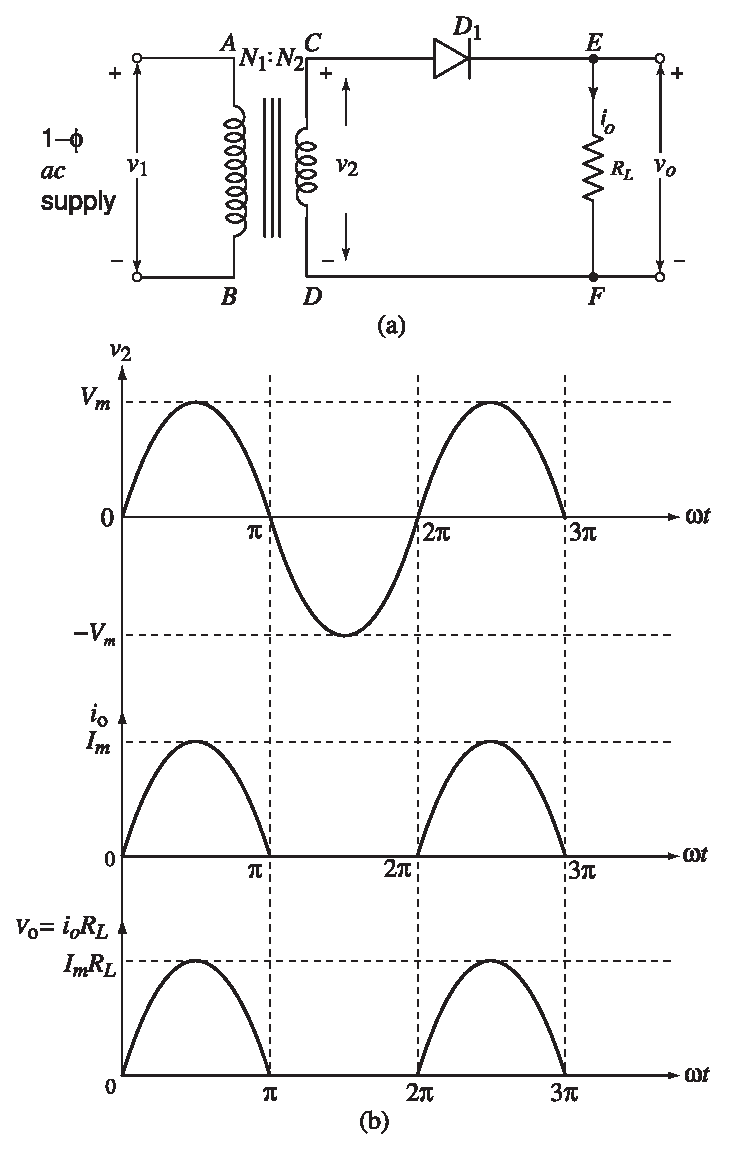
\includegraphics[scale=.8]{chap2/add-fig/S3-EE-02-001ab.eps}
\caption{(a) Half-wave rectifier. (b) Waveforms of transformer secondary voltage, load current and load voltage}\label{fig2.1}
\end{figure}

Half-wave rectifier\index{Rectifier!half-wave rectifier}\index{Half-wave rectifier} rectifies only one half-cycle of the $ac$
input. Fig.~\ref{fig2.1}(a) shows the circuit of a half-wave rectifier and
Fig.~\ref{fig2.1}(b) shows the waveforms of transformer secondary voltage, load
current and load voltage.
\begin{align}
v_1 & = V_m \sin \omega t~; \quad \text{ instantaneous supply
  voltage} \label{eq2.1}\\[4pt]
v_2 & = \frac{N_2}{N_1} \, v_1 \label{eq2.2}\\[4pt]
v_2 & = \frac{N_2}{N_1}\, V_m \sin \omega\, t~; \quad \text{ instantaneous
  secondary voltage} \label{eq2.3}
\end{align}

The required $dc$ voltage is typically 5\,V to 25\,V, but the available
$ac$ supply is 230 V at 50 Hz. A stepdown  transformer is used to
reduce the available $ac$ voltage to the required level. $R_L$
represents the load which consumes power from the rectifier.

The polarities shown in Fig.~\ref{fig2.1}(a) are instantaneous. Refer
Fig.~\ref{fig2.1}(a), during the positive half-cycle of $ac$ supply, the
voltage at point $C$ is positive. Hence, diode conducts and the
current $i_o$ follows the path $C$-$D_1$-$E$-$F$-$D$-$C$. The load
voltage $v_o = i_o\, R_L$.

During the negative half-cycle of $ac$ supply, the voltage at point
$C$ is negative. Therefore the diode gets reverse biased and the
current $i_o$ is zero and as a result. $v_o =0$. Note that the load
current flows only for the positive half-cycle of input and is zero for the
negative half-cycle.

\section{Expressions for (a) Average\,/\,DC load current and load voltage\newline (b) RMS load current and load voltage}\label{sec2.3}

\smallskip

\heading{(a) Average\,/\,DC load current\index{Half-wave rectifier!dc load current} or output current}

Let us write the equation for instantaneous load current using the
equivalent circuits.
\begin{figure}[H]
\centering
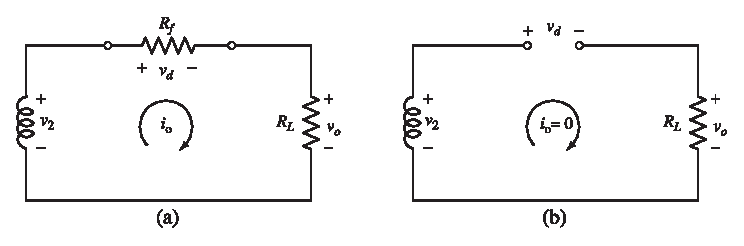
\includegraphics{chap2/add-fig/S3-EE-02-002ab.eps}
\caption{(a) Equivalent circuit when diode is conducting. (b) Equivalent circuit when the diode is not conducting}\label{fig2.2}
\end{figure}

The conducting diode can be replaced by its $on$-state resistance
$R_f$ as shown in Fig. 2.2(a) and the non-conducting diode can be
replaced by an open circuit as shown in Fig. 2.2(b).

From the circuit of Fig. 2.2(a)
\begin{equation}
i_o = \frac{v_2}{R_f + R_L}~;\quad 0\leq \omega t \leq \pi \label{eq2.4}
\end{equation}
and from the circuit of Fig. 2.2(b)
\begin{equation}
i_o = 0~;\quad \pi\leq \omega t\leq 2\pi \label{eq2.5}
\end{equation}

From equation \eqref{eq2.3}, $v_2 = \dfrac{N_2}{N_1}\, V_m \sin \omega t$.

Taking $N_2/ N_1 = 1$  we have, $v_2 = V_m \sin \omega t$.

Using this relation in equations \eqref{eq2.4} and \eqref{eq2.5} we can rewrite the
equations as 
\begin{align}
i_o & = \begin{cases}
I_m \sin \omega\,t & ; ~ 0 \leq \omega t \leq \pi\\
0  & ; ~ \pi \leq \omega t < 2 \pi
  \end{cases} \label{eq2.6}\\
\text{where } \quad I_m & = \frac{V_m}{R_f + R_L}\label{eq2.7}
\end{align}

$I_m$ is the peak load current/peak diode current.

\smallskip
{\bf Average\,/\,DC load current, \boldmath$I_{dc}$~:}

Referring to Fig. 2.1(b), average\,/\,DC load current is given by
\begin{align}
I_{dc} & = \frac{\text{Area under one cycle of $i_o$}}{\text{Period of
  $i_o$}}\notag\\[4pt]
& = \int\limits^{2\pi}_0 \frac{i_o\,d \omega t}{2 \pi}\notag\\[4pt]
& = \frac{1}{2\pi} \left[\int\limits^\pi_0 I_m \sin \omega t ~ d \omega
  t + \int\limits^{2\pi}_\pi 0 ~ d \omega t\right]\notag\\[4pt]
& = \frac{I_m}{2\pi} \ [-\cos \omega t]^{\pi}_0\notag\\[4pt]
& = \frac{I_m}{2\pi} \ [-\cos \pi + \cos 0]\notag\\[4pt]
I_{dc} & = \frac{I_m}{\pi} \label{eq2.8}
\end{align}

\eject

\heading{Average\,/\,DC load voltage,\index{Half-wave rectifier!dc load voltage} $V_{dc}$\,:}
\begin{align}
V_{dc} & = I_{dc}\, R_L \notag\\[5pt]
& = \left[\frac{I_m}{\pi} \right] R_L \notag\\[5pt]
& = \frac{1}{\pi} \left[\frac{V_m}{R_f + R_L} \right] R_L \notag\\[5pt]
V_{dc} & = \frac{V_m /\pi}{1+ R_f /R_L}\label{eq2.9}
\end{align} 

\heading{RMS load current,\index{Half-wave rectifier!rms load current} $I_{rms}$\,:}
\begin{align}
I_{rms} & = \sqrt{\frac{\text{Area under one cycle of
      $i^2_o$}}{\text{Period of $i_o$}}}\notag\\[5pt]
& = \sqrt{\frac{\int^{2\pi}_0 i^2_0\, d\omega t}{2 \pi}} \notag\\[5pt]
& = \sqrt{\frac{1}{2\pi} \left\{\int\limits^\pi_0 I^2_m \sin^2 d \omega
   t + \int\limits^{2\pi}_\pi 0\; d \omega t\right\}} \notag\\[5pt]
& = I_m \sqrt{\frac{1}{2\pi} \int\limits^\pi_0 \frac{1}{2} [1-\cos 2
    \omega t]\; d \omega t } \qquad \left[\because ~~ \sin^2 \omega t =
  \frac{1 - \cos  2 \omega t}{2} \right] \notag\\[5pt]
& = I_m \sqrt{\frac{1}{4 \pi} \left[\int\limits^\pi_0 d \omega t -
   \int\limits^\pi_0 \cos 2 \omega t\; d \omega t \right]}\notag\\[5pt]
& = \frac{I_m}{2} \sqrt{\frac{1}{\pi} \left\{(\omega t)^\pi_0 - \left(
  \frac{\sin 2 \omega t}{2}  \right)^\pi_0 \right\}} \notag\\[5pt]
& = \frac{I_m}{2} \sqrt{\frac{1}{\pi} \left\{(\pi - 0) - \frac{1}{2}
  (\sin 2 \pi - \sin 0) \right\}} \notag\\[5pt]
I_{rms} & = \frac{I_m}{2}\label{eq2.10}
\end{align}

\eject

\heading{RMS load voltage,\index{Half-wave rectifier!rms load voltage} $V_{rms}$\,:}
\begin{align}
V_{rms} & = I_{rms}\, R_L \notag\\[4pt]
& = \left[\frac{I_m}{2} \right] R_L \notag\\[4pt] 
& = \frac{1}{2} \left[\frac{V_m}{R_f + R_L} \right] R_L \notag\\[4pt]
V_{rms} & = \frac{V_m/2}{1 + R_f /R_L} \label{eq2.11}
\end{align}

\medskip
\noindent\textbf{Note:}

If the diode is ideal, $R_f= 0$.
\begin{itemize}
\itemsep=0pt
\item
Then, from equation \eqref{eq2.7}, $I_m = V_m / R_L$
\item
From equation \eqref{eq2.9}, $V_{dc} = V_m/\pi$
\item
From equation \eqref{eq2.11}, $V_{rms}= V_m /2$.
\end{itemize}

\begin{example}\label{exam2.1}
Show that in a half-wave rectifier, the $dc$ voltage across the diode
is equal but opposite in polarity of the $dc$ voltage across $R_L$.
\end{example}

\begin{solution}
From the circuit of Fig. 2.2 (a), the instantaneous diode voltage,
\begin{equation*}
v_d = i_o\, R_f \tag{A}
\end{equation*}

But from equation \eqref{eq2.6}
$$
i_o = I_m \sin \omega t, \quad 0 \leq \omega t \leq \pi
$$

Using this relation in equation (A), we have 
\begin{equation*}
v_d = I_m\, R_f \sin \omega t, \quad 0 \leq \omega t \leq \pi \tag{B}
\end{equation*}

Also applying Kirchhoff's Voltage Law to the circuit of Fig. 2.2(b)
\begin{equation*}
v_2 - v_d - v_o = 0, \quad \pi \leq \omega t \leq 2 \pi \tag{C}
\end{equation*}

But in the interval, $\pi \leq \omega t \leq 2 \pi$, \quad $v_o = i_o\;
R_L = 0$
\begin{equation*}
\therefore~~ v_d = v_2 = V_m \sin \omega t, \quad \pi \leq \omega t
\leq 2 \pi \tag{D}
\end{equation*}

Combining equations (B) and (D) we have
$$
v_d = \begin{cases}
I_m\, R_f \sin \omega t  &;~~~ 0 \leq \omega t \leq \pi\\
V_m \sin \omega t  &;~~~ \pi \leq \omega t \leq 2 \pi
\end{cases}
$$ 

Fig. A shows the voltage waveform across diode, $v_d$. While drawing
the waveform $v_d$, we have assumed, $R_f = 0$.
\begin{figure}[H]
\centering
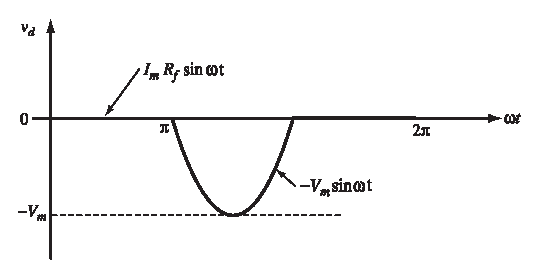
\includegraphics{chap2/add-fig/S3-EE-02-003.eps}

\smallskip

\colorbox{lightgray}{{\bf Fig.~A~:} \em Waveform of voltage across diode}
\end{figure}

Average or $dc$ voltage across diode,
\begin{align*}
V'_{dc} & = \frac{\text{Area under the waveform of
    $v_d$}}{\text{Period of $v_d$}}\\
& = \frac{\int\limits^{2\pi}_0 v_d \; d \omega t}{2 \pi}\\
& = \frac{1}{2 \pi} \left[\int\limits^{2\pi}_\pi V_m \sin \omega
  t \ d \omega t \right]\\
& = \frac{1}{2 \pi}\, [V_m (-\cos \omega t)^{2 \pi}_\pi]\\
& = \frac{1}{2 \pi}\, [V_m (-\cos 2 \pi + \cos \pi)]=-\dfrac{V_{m}}{\pi}
\end{align*}

Since, from equation \eqref{eq2.7}, $V_m = I_m (R_f + R_L)$ and $R_f$ is being
considered as zero, we get
\begin{align*}
V'_{dc} & = -\frac{V_m}{\pi} = \frac{-I_m\, R_L}{\pi}\\
& = - I_{dc}\, R_L\\
V'_{dc} & = - V_{dc} \tag{E}
\end{align*}
Equation (E) shows that the $dc$ diode voltage is equal but opposite in
polarity of the DC load voltage.
\end{solution}

\section{Percentage regulation}\label{sec2.4}

The variation of $dc$ output voltage as a function of DC load current
is called regulation.\index{Regulation} The percentage regulation is defined as 
\begin{equation}
\% ~~ \text{Regulation} = \frac{V_{\text{No load}} -
  V_{\text{load}}}{V_{\text{load}}} \times 100 \label{eq2.12}
\end{equation}
where $V_{\text{No load}}$  is the $dc$ output voltage when load
current is zero and $V_{\text{load}}$ is the $dc$ output voltage when
the load current is equal to normal load current.

Ideally, the $dc$ output voltage is independent of load current.
$$
\therefore ~~ V_{\text{No load}} = V_{\text{load}}
$$

Hence,
$$
\% ~\text{ Regulation } = 0
$$

\subsection{Expression for percentage regulation of half wave
  rectifier}\label{subsec2.4.1}
\index{Half-wave rectifier!regulation}

Consider equation \eqref{eq2.9}
$$
V_{dc} = \frac{\frac{V_m}{\pi}}{1 + \frac{R_f}{R_L}}
$$

The above equation gives the $dc$ output voltage when $R_L$ is drawing
normal load current.
\begin{equation}
\therefore ~~~ V_{dc} = V_{\text{load}} = \frac{\frac{V_m}{\pi}}{1 +
  \frac{R_f}{R_L}} = \frac{\left(\frac{V_m}{\pi} \right) R_L}{R_f+  R_L} \label{eq2.13}
\end{equation}

Under No load, the load current is zero since $R_L = \infty$

From equation \eqref{eq2.13} with  $R_L = \infty$, we get
\begin{equation}
V_{\text{No load}} = \left[ \frac{V_m}{\pi} \right] \label{eq2.14}
\end{equation}

Substituting equations \eqref{eq2.13} and \eqref{eq2.14} in equation
\eqref{eq2.12}
\begin{align}
\% ~ \text{Regulation } & = \frac{\frac{V_m}{\pi} -
  \frac{\left(\frac{V_m}{\pi} \right) R_L}{R_f + R_L}}{
  \left(\frac{V_m}{\pi} \right) \frac{R_L}{(R_f + R_L)}} \times 100 \notag\\[4pt]
& = \frac{1- \frac{R_L}{R_f + R_L}}{\frac{R_L}{R_f + R_L}} \times
100 \notag\\[4pt]
& = \frac{R_f + R_L - R_L}{R_L} \times 100 \notag\\[4pt]
\% ~ \text{ Regulation } & = \frac{R_f}{R_L} \times 100 \label{eq2.15}
\end{align}

For an ideal diode, $R_f = 0$. From equation \eqref{eq2.15} we get
$$
\% ~ \text{ Regulation = 0}
$$
{\em Therefore with an ideal diode, a half-wave rectifier behaves as an
ideal $dc$ power supply.}

\section{Rectification efficiency}\label{sec2.5}

Rectification efficiency\index{Rectification efficiency} is defined as the ratio of the $dc$ output
power to $ac$ input power supplied to the rectifier. It is denoted by
$\eta_r$.
\begin{equation}
\eta_r = \frac{P_{dc}}{P_i} \label{eq2.16}
\end{equation}
where,

$P_{dc}$ is the $dc$ output power of the rectifier

$P_i$ is the $ac$ input power to the rectifier.

\subsection{Expression for rectification efficiency of half wave
  rectifier}\label{subsec2.5.1}
\index{Half-wave rectifier!rectification efficiency}

DC output power of the rectifier is given by, 
$$
P_{dc} = [I_{dc}]^2 R_L
$$

For a half-wave rectifier,
\begin{align}
I_{dc} & = \left[\frac{I_{m}}{\pi} \right] \notag\\
\therefore ~~ P_{dc} & = \frac{I^2_m\; R_L}{\pi^2} \label{eq2.17}
\end{align}
$ac$ power input to the rectifier is given by 
\begin{equation}
P_i = [I_{rms}]^2 [R_f + R_L] \label{eq2.18}
\end{equation}

\eject

But
$$
I_{rms} = \frac{I_m}{2}
$$

Using this relation in equation \eqref{eq2.18} we have,
\begin{equation}
P_i = \frac{I^2_m}{4}\, [R_f + R_L] \label{eq2.19}
\end{equation}

Substituting equations \eqref{eq2.17} and \eqref{eq2.19} in equation
\eqref{eq2.16}, we get
\begin{align}
\eta_r & = \frac{\left[\frac{I^2_m R_L}{\pi^2} \right]}{\frac{I^2_m[R_{f}+R_{L}]}{4}} = \frac{0.406 R_L}{R_f + R_L} \notag\\[4pt]
\% ~~ \eta_r & = \frac{40.6}{1+\frac{R_f}{R_L}}  \label{eq2.20}
\end{align}

If the diode is ideal, $R_f = 0$
\begin{equation}
\therefore~~ \% ~ \eta_{r \max} = 40.6 \label{eq2.21}
\end{equation}

\medskip
\noindent
\textbf{Note:}

Consider equation \eqref{eq2.21}
\begin{align*}
\eta_{r \max} & = \frac{P_{dc}}{P_i} = 0.406\\
P_{dc} & = 0.406\, P_i
\end{align*}

{\em The $dc$ output power is only 40.6\% of the $ac$ input power. The
remaining 59.4\% of $ac$ input power goes unused. Hence half-wave
rectifier has a very poor rectification efficiency.}

\begin{example}\label{exam2.2}
Show that the maximum $dc$ output power $P_{dc} = V_{dc}\,I_{dc}$ in a
half-wave rectifier occurs when the load resistance $R_L$ equals the
diode forward resistance $R_f$.
\end{example}

\begin{solution}
$$
P_{dc} = V_{dc}\,I_{dc}
$$

But
\begin{align*}
I_{dc} & = \frac{V_{dc}}{R_L} \\[4pt]
\therefore ~~ P_{dc}  & = \frac{V^2_{dc}}{R_L} \tag{A}
\end{align*}

From equation \eqref{eq2.9},
\begin{align*}
V_{dc} & = \frac{\left[\frac{V_m}{\pi} \right]}{1+ \frac{R_f}{R_L}}\\[4pt]
& = \frac{\left[\frac{V_m}{\pi} \right]R_L}{R_f + R_L}
\end{align*}

Substituting this relation in equation (A), we have
\begin{align*}
P_{dc} & = \left[\frac{\left[\frac{V_m}{\pi} \right] R_L}{R_f+R_L}\right]^2 \times \frac{1}{R_L}\\
& = \frac{\left[\frac{V_m}{\pi} \right]^2 R_L}{(R_f + R_L)^2} \tag{B}
\end{align*}

Note that $P_{dc}$ is a function of $R_L$. To obtain the value of
$R_L$ which results in maximum $P_{dc}$, set~ $\dfrac{dP_{dc}}{dR_L} =0$.
\begin{align*}
\frac{dP_{dc}}{dR_L} = \left[\frac{V_m}{\pi} \right]^2
\left[\frac{(R_f + R_L)^2 (1) - 2 R_L (R_f + R_L)}{ (R_f + R_L)^4} \right]
& = 0\\[4pt]
(R_f + R_L)^2 - 2 R_L (R_f + R_L) & = 0 \\[4pt]
(R_f + R_L) \times (R_f + R_L - 2 R_L) & = 0\\[4pt]
(R_f + R_L) (R_f-R_L) & = 0\\[4pt]
\text{Since } (R_f + R_L) \neq 0 ~~ \text{ then, } ~~ R_f - R_L & = 0\\[4pt]
\text{or } R_L & = R_f \tag{C}
\end{align*}

\medskip
\noindent\textbf{Note:}

To obtain maximum value of $P_{dc}$, we have to substitute $R_L=R_f$
in equation (B).
\begin{align*}
P_{dc \max} & = \frac{\left(\frac{V_m}{\pi} \right)^2 R_L }{(R_L +
  R_L)^2}\\[4pt]
& = \frac{V^2_{dc}}{4R_{L}}\\[4pt]
\text{or}\qquad P_{dc \max} & = \frac{V^2_{dc}}{4 R_f} \tag{D}
\end{align*}
\end{solution}

\eject

\section{Ripple factor}\label{sec2.6}

Ripple factor\index{Ripple factor} is the ratio of RMS value of $ac$ component present in
the rectified output to the $dc$ component of the rectified output. It
is denoted by $\gamma$.
\begin{equation}
\gamma = \frac{V_{ac}}{V_{dc}} \label{eq2.22}
\end{equation}

$V_{ac}$ is the RMS value of $ac$ component present in the rectified
output.

$V_{dc}$ is the $dc$ component of rectifier.

\subsection{Ripple factor of half wave rectifier}\label{subsec2.6.1}
\index{Half-wave rectifier}\index{Ripple factor!half wave rectifier}

The output of rectifier is a pulsuating $dc$ which has 
\begin{itemize}
\item[(a)] an $ac$ component of RMS value $V_{ac}$ and

\item[(b)] a $dc$ component $V_{dc}$.
\end{itemize}

As the total power output is the sum of powers of $dc$ and $ac$
components, we can write
\begin{align*}
\begin{bmatrix}
\text{The total RMS value of }\\
\text{rectified output}
\end{bmatrix}^2 & = 
\begin{bmatrix}
dc \text{~ value}
\end{bmatrix}^2 + 
\begin{bmatrix}
\text{RMS value of}\\
ac \text{~ component}
\end{bmatrix}^2\\
(V_{rms})^2 & = (V_{dc})^2 + (V_{ac})^2
\end{align*}
 
Dividing throughout by $V^2_{dc}$ we get
\begin{equation}
\left[
\frac{V_{rms}}{V_{dc}} 
\right]^2 = 1 + 
\left[
\frac{V_{ac}}{V_{dc}}
\right]^2
\label{eq2.23}
\end{equation}

But
\begin{align}
\gamma & = V_{ac}/V_{dc}\notag\\[4pt]
\therefore ~~ \left[\frac{V_{rms}}{V_{dc}} \right]^2 & = 1 +
\gamma^2 \notag\\[4pt]
\text{or } \quad \gamma & = \sqrt{\;\left[\frac{V_{rms}}{V_{dc}}
    \right]^2 - 1}\label{eq2.24}\\[4pt]
\text{But}\qquad V_{rms} & = \frac{\left[\frac{V_m}{2} \right]}{1+\frac{R_f}{R_L}}
\notag 
\end{align}
\begin{align*}
\text{and}\qquad V_{dc} & = \frac{\left[\frac{V_m}{\pi} \right]}{1+ \frac{R_f}{R_L}}\\
\therefore ~~ \left[\frac{V_{rms}}{V_{dc}} \right] & = \frac{\pi}{2}
\end{align*}

Using this relation in equation \eqref{eq2.24}, we have
\begin{align*}
\gamma & = \sqrt{\left(\frac{\pi}{2} \right)^2 -1}\\
\gamma & = 1.21
\end{align*}
\noindent{\textbf{Note:}}
\vskip -.7cm
\begin{align*}
\gamma & = 1.21 = \left[\frac{V_{ac}}{V_{dc}} \right]\\
V_{ac} & = 1.21 V_{dc}
\end{align*}

{\em In a half-wave rectifier, the $ac$ or ripple component is 121\% of the
$dc$ component i.e. $ac$ component is greater than $dc$
component. Hence, half-wave rectifier is not recommended for practical
applications.}

\section{Peak inverse voltage}\label{sec2.7}

Peak inverse voltage\index{Peak inverse voltage} (PIV) is the maximum reverse voltage to which the
diode can be subjected. If the applied reverse voltage across the
diode is greater than its PIV rating, the reverse breakdown of the
diode occurs which causes a permanent damage to the diode.\\[-.7cm]

\subsection{Peak inverse voltage of half wave
  rectifier}\label{subsec2.7.1}
\index{Half-wave rectifier!peak inverse voltage}

The equivalent circuit of a half-wave rectifier when the diode is not
conducting is shown in Fig.~\ref{fig2.3}.
\vskip -.5cm
\begin{figure}[H]
\centering
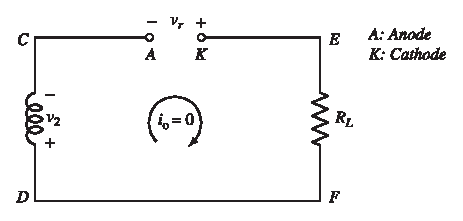
\includegraphics{chap2/add-fig/S3-EE-02-IN001.eps}
\caption{Circuit to find PIV of half wave rectifier}\label{fig2.3}
\end{figure}
$v_r$ is the instantaneous reverse voltage across the diode.

\vfill\eject

Writing Kirchhoff's Voltage Law equation to the circuit of Fig.~\ref{fig2.3}, we have
$$
-v_2 + v_r - i_o\, R_L =0
$$

Since, $i_o = 0$, $v_r = v_2 = V_m \sin \omega t$ 
$$
PIV = v_{r \max} = V_m, \quad \text{ when } \sin \omega t = 1
$$

{\em Therefore PIV for a half-wave rectifier is equal to the peak secondary
voltage of the transformer.}

\section{Summary of results for half-wave rectifier}\label{sec2.8}

The results derived for half-wave rectifier are summarised in Table~\ref{tab2.1}.
\begin{table}[H]
\caption{Summary of results for half-wave rectifier}\label{tab2.1}
\renewcommand{\arraystretch}{1.3}
\tabcolsep=9pt
\begin{tabular}{|c|c|c|}
\hline
\multirow{2}{1.5cm}{Parameter}\index{Half-wave rectifier!parameter} & \multicolumn{2}{c|}{Expression}\\\cline{2-3}
& Practical diode & Ideal diode $(R_f=0)$\\
\hline
&&\\[-14pt]
Peak load\,/\,diode current, $I_m$ & $\dfrac{V_m}{R_f + R_L}$ &
$\dfrac{V_m}{R_L}$\\[7pt]
\hline
&&\\[-14pt]
DC load current, $I_{dc}$ & $\dfrac{V_m/\pi}{R_f + R_L} =
\dfrac{I_m}{\pi}$ & $\dfrac{V_m/\pi}{R_L}$\\[7pt]
\hline
&&\\[-14pt]
RMS load current, $I_{rms}$ & $\dfrac{V_m/2}{R_f+R_L} =
\dfrac{I_m}{2}$  & $\dfrac{V_m}{2}$\\[7pt]
\hline
&&\\[-14pt]
DC load voltage, $V_{dc}$ & $\dfrac{V_m/\pi}{1+ R_{f}/R_L}$ &
$\dfrac{V_m}{\pi}$\\[7pt]
\hline
&&\\[-14pt]
RMS load voltage, $V_{rms}$ & $\dfrac{V_m /2}{1 + R_f / R_L}$ &
$\dfrac{V_m}{2}$\\[7pt]
\hline
&&\\[-14pt]
$\%$ Regulation & $\dfrac{R_f}{R_L} \times 100$ & 0\\[7pt]
\hline
Ripple factor, $\gamma$ & 1.21 & 1.21\\
\hline
&&\\[-14pt]
Rectification efficiency, $\eta_r$ & $\dfrac{0.406}{1+R_f /R_L}$ &
0.406  or 40.6 \% \\[7pt]
\hline
Peak inverse voltage, PIV & $V_m$ & $V_m$\\
\hline
\end{tabular}
\end{table}

\noindent{\textbf{Note:}}
In all numerical examples, wherever not specified the transformer
turns ratio, $N_1/N_2$, is taken as unity. 

\eject

\begin{example}\label{exam2.3}
A diode whose internal resistance is 20 $\Omega$, is used to supply
power to a\break 1000 $\Omega$ load from a 110 V (rms) source of
supply. Calculate
\begin{itemize}
\item[(a)] Peak load current

\item[(b)] DC load current

\item[(c)] AC load current 

\item[(d)] DC diode voltage

\item[(e)] Total input power to the circuit

\item[(f)] Percentage regulation from no load to the given load. 
\end{itemize} 
\end{example}


\begin{solution}
Given 
\begin{align*}
R_f =20\, \Omega, \ R_L & = 1000 \Omega\\
\text{Assume, \ } \frac{N_1}{N_2} & = 1\\
\frac{v_1}{v_2} & = \frac{N_1}{N_2} = 1\\
\therefore ~~~ V_2 & = V_1 = 110 \V\\
V_m & = \sqrt{2} V_{2}=\sqrt{2}\times 110 \V\\
& = 155.56 \V 
\end{align*}

\begin{itemize}
\item[(a)] Peak load current,
\begin{align*}
I_m & = \frac{V_m}{R_f + R_L}\\
& = \frac{155.56 \V}{20\,\Omega + 1000\,\Omega}\\[5pt]
I_m & = 152.5 \mA
\end{align*}

\item[(b)] DC load current,
\begin{align*}
I_{dc} & = \frac{I_m}{\pi}\\
& = \frac{152.5 \mA}{\pi}\\
I_{dc} &  = 48.54 \mA
\end{align*}

\itemsep=2pt
\item[(c)] AC load current or RMS load current,
\begin{align*}
I_{rms} & = \frac{I_m}{2}\\
& = \frac{152.5 \mA}{2}\\
& = 76.25 \mA
\end{align*}

\item[(d)] DC diode voltage,
\begin{align*}
V'_{dc} & = - V_{dc}\\
& = - I_{dc}\, R_L\\
& = - (48.56 \mA) (1 k\Omega)\\
& = - 48.54 \V
\end{align*}

\item[(e)] Total power input to the circuit,
\begin{align*}
P_i & = (I_{rms})^2 [R_f + R_L]\\
& = [76.25 \times 10^{-3}]^2\; [20\,\Omega + 1000\,\Omega]\\
& = 5.93 \W
\end{align*}

\item[(f)] Percentage regulation,
\begin{align*}
\% ~ Regulation &  = \frac{R_f}{R_L} \times 100\\
& = \frac{20 \Omega}{1000 \Omega} \times 100\\
& = 2
\end{align*}
\end{itemize}
\vskip -1cm
\end{solution}

\begin{example}\label{exam2.4}
The input to a half-wave rectifier is given through a 10:1 transformer
from a supply given by 230 sin 314t V. If $R_f = 50\,\Omega$ and $R_L =
500\,\Omega$ determine
\begin{itemize}
\itemsep=1pt
\item[(a)] DC load voltage
\item[(b)] RMS load voltage 
\item[(c)] PIV across the diode 
\item[(d)] Rectification efficiency
\item[(e)] DC power delivered to the load 
\item[(f)] Frequency of output waveform
\end{itemize}
\end{example}

\begin{solution}
Given,
\begin{align*}
v_1 & = 230 \sin 314 t \V, \quad \frac{N_1}{N_2} = 10\\
R_f & =  50 \Omega \quad R_L = 500 \Omega\\
\frac{v_1}{v_2} & = \frac{N_1}{N_2}\\
v_2 & = (N_2/N_1)\, v_1\\
& = \left(\frac{1}{10} \right) 230 \sin 314 t \V  = 23 \sin 314 t \V\\
\text{we have } ~~ v_2 & = 23 \sin 314 t \V  = V_m \sin \omega t \V\\
\end{align*}
on comparision, we get 
\begin{align*}
V_m & = 23 \V , ~~ \omega = 314\, r/s\\
\omega & = 2 \pi f\\
f & = \frac{\omega}{2 \pi} = 50 Hz
\end{align*}

\begin{itemize}
\item[(a)] DC load voltage,
\begin{align*}
V_{dc} & = \frac{V_m/\pi}{1 + R_f / R_L} \\
& = \frac{23 V/\pi}{1 + (50\,\Omega/ 500\,\Omega)} = 6.66 \V
\end{align*}

\item[(b)] RMS load voltage, 
\begin{align*}
V_{rms} & = \frac{V_{m}/2}{1 + R_f / R_L}\\
& = \frac{23 V/2}{1 + (50\,\Omega/ 500\,\Omega)} = 10.45 \V
\end{align*}

\item[(c)] PIV across the diode,
\begin{align*}
PIV & = V_m = 23 \V
\end{align*}

\item[(d)] Rectification efficiency,
\begin{align*}
\% ~~ \eta_r & = \frac{40.6}{1 + \frac{R_f}{R_L}}\\
& = \frac{40.6}{1+ (50\,\Omega /500\,\Omega)} = 36.91
\end{align*}

\item[(e)] $dc$ power delivered to the load.
\begin{align*}
P_{dc} & = \frac{V^2_{dc}}{ R_L} = \frac{(6.66 V)^2}{500\,\Omega}\\
& = 0.0887 \W \text{~ or ~} 88.7 \text{~mW}
\end{align*}

\item[(f)] Frequency of output waveform is same as the supply
  frequency i.e. 50 Hz.
\end{itemize}
\vskip -.9cm
\end{solution}

\section{Full-wave rectifier using two diodes and a centre-tapped transformer}\label{sec2.9}\index{Full-wave rectifier}
\vskip -.7cm
\begin{figure}[H]
\centering
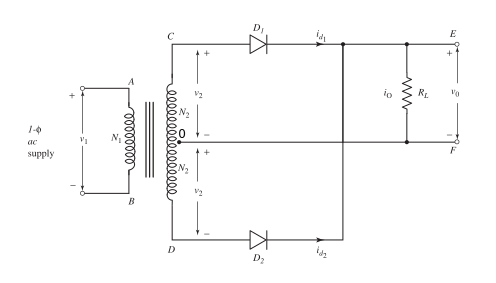
\includegraphics{chap2/add-fig/S3-EE-02-004.eps}
\caption{Full-wave rectifier, using two diodes and a centre-tapped transformer}\label{fig2.4}
\end{figure}

Fig.~\ref{fig2.4} shows the circuit of Full-wave rectifier\index{Rectifier!full-wave rectifier} using two diodes and
a centre tapped transformer.
\begin{align*}
& v_1  = V_m \sin \omega t \V\\
& v_2  = (N_2 / N_1) v_1 = (N_2 /N_1) V_m \sin \omega t \V\\
& v_1 \text{ is the instantaneous ac supply voltage}\\
& v_2 \text{ is the instantaneous secondary voltage}\\
& N_1/N_2 \text{ is the turns ratio of transformer}
\end{align*}
\begin{figure}[H]
\centering
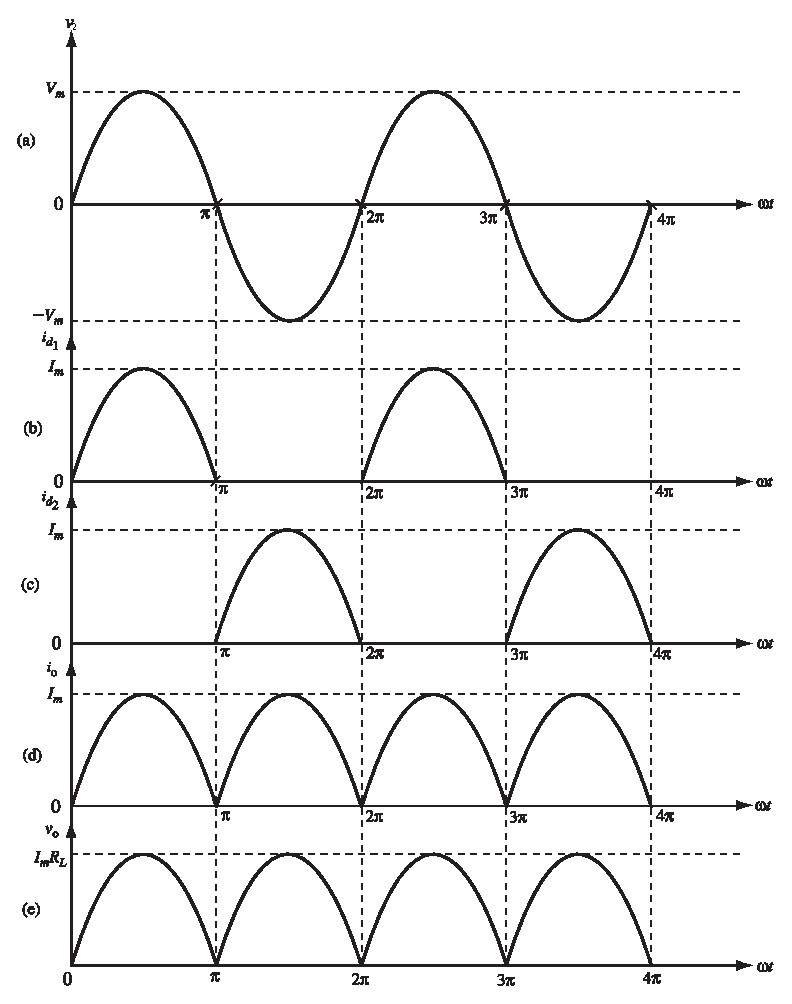
\includegraphics{chap2/add-fig/S3-EE-02-005.eps}
\caption{Voltage and current waveforms. (a) Secondary voltage waveform, (b) \&\ (c) Diode current waveforms, (d) Load current waveform, (e) Load voltage waveform}\label{fig2.5}
\end{figure}

\eject

A step down transformer is used to reduce the $ac$ supply voltage to
the required level. Centre tapping in the secondary of the transformer
is done to obtain two equal voltages but of opposite phase.

During the positive half-cycle of the $ac$ supply, the voltage at
point $C$ is positive and the voltage at point $D$ is
negative. Consequently, Diode $D_1$ conducts and $D_2$ remains
off. The current follows the path $C-D_1-E-F-O-C$. Hence, during the
positive-half cycle, $i_o  = i_{d1}$.

During the negative half-cycle of the $ac$ supply, the voltage at
point $D$ is positive and the voltage at point $C$ is negative. Thus,
$D_2$ conducts and $D_1$ is \textit{off}. Accordingly, the current
follows the path $D-D_2 - E-F -O-D$. This means that during the
negative-half cycle, $i_o = i_{d_2}$.

Note that during both half-cycles of $ac$ supply, the load current
$i_0$ flows from $E$ to $F$. Hence, $i_o$ is unidirectional.

The various voltage and current waveforms are shown in Fig.~\ref{fig2.5}.

\section{Expressions for (a) DC load current and load voltage
(b) RMS load current and load voltage of full wave rectifier}\label{sec2.10}

From the waveform of load current $i_o$, shown in Fig. 2.5(d), we find
that $i_o$ repeats once in every $\pi$ rad. Hence, period of $i_o$ waveform is
$\pi$ rad.

Let us assume that $D_1$ is conducting and $D_2$ is \textit{off}. From
the circuit of Fig.~\ref{fig2.4}, making use of this fact, we get the equivalent
circuit shown in Fig.~\ref{fig2.6}.
\begin{figure}[H]
\centering
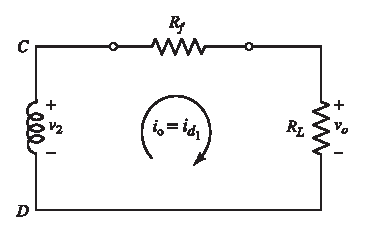
\includegraphics{chap2/add-fig/S3-EE-02-006.eps}
\caption{Equivalent circuit during positive half-cycles of $ac$ supply}\label{fig2.6}
\end{figure}

From Fig.~\ref{fig2.6},
\begin{align}
i_o & = \frac{v_2}{R_f + R_L} \notag\\
\text{But, } ~ ~v_2 & = \left(\frac{N_2}{N_1} \right) V_m \sin \omega
t. \quad \text{Assuming }~~~ \frac{N_1}{N_2} = 1, \notag\\
\text{we have, } ~~~ v_2 & = V_m \sin \omega t \notag\\[4pt]
\text{Now, } ~~~ i_o & = \frac{V_m}{R_f + R_L} \sin \omega
t  \label{eq2.25}\\[4pt]
i_o & = I_m \sin \omega t, \quad 0 \leq \omega t \leq \pi \notag\\[4pt]
\text{ where, ~~} I_m & = \frac{V_m}{R_f + R_L} \label{eq2.26}
\end{align}

$I_m$ is the peak load current/peak diode current.

\smallskip

\heading{DC load current, \ \boldmath$I_{dc}$\,:}\index{Full-wave rectifier!dc load current}
\begin{align}
I_{dc} & = \frac{\text{Area under one cycle of $i_o$}}{\text{Base}} \notag\\[4pt]
& = \frac{\int\limits^\pi_0 i_0\; d \omega t}{\pi} \notag\\[4pt]
& = \frac{1}{\pi} \int\limits^{\pi}_0 I_m \sin \omega t~ d \omega t \notag\\[4pt]
& = \frac{I_m}{\pi} [-\cos \omega t]^\pi_0 \notag\\[4pt]
& = \frac{I_m}{\pi} [-\cos \pi + \cos 0]\notag\\[4pt]
I_{dc} & = \frac{2 I_m}{\pi} \label{eq2.27}
\end{align}

\heading{DC load voltage, \ \boldmath$V_{dc}$\,:}\index{Full-wave rectifier!dc load voltage}
\begin{align}
V_{dc} & = I_{dc}\; R_L \notag\\[4pt]
& = \frac{2I_m}{\pi}\;{R_L}\notag\\[4pt]
& = \frac{2}{\pi} \left[\frac{V_m}{R_f+ R_L} \right] R_L \notag\\[4pt]
V_{dc} & = \frac{\frac{2V_m}{\pi}}{1+ \frac{R_f}{R_L}} \label{eq2.28}
\end{align}

Comparing equations \eqref{eq2.9} and \eqref{eq2.28}, we find  that the $dc$ output
voltage in a full-wave rectifier is twice that of half-wave rectifier.

\vfill\eject

\heading{RMS load current, \ \boldmath$I_{rms}$\,:}\index{Full-wave rectifier!rms load current}
\begin{align}
I_{rms} & = \sqrt{\frac{\text{Area under one cycle of
    $i^2_o$}}{\text{Base}}} \notag\\
& = \sqrt{\frac{1}{\pi} \int\limits^\pi_0 i^2_0\; d \omega t} \notag\\
& = \sqrt{\frac{1}{\pi} \int\limits^\pi_0 I^2_m \sin^2 \omega t \; d
  \omega t} \notag\\
& = I_m \sqrt{ \frac{1}{\pi} \int\limits^\pi_0 \frac{1}{2} [1-\cos 2
    \omega t]\; d \omega t} \notag\\
& = I_m \sqrt{\frac{1}{2 \pi} \left\{ \int\limits^\pi_0 d \omega t -
  \int\limits^\pi_0 \cos 2 \omega t \; d \omega t\right\}} \notag\\
& = I_m \sqrt{\frac{1}{2\pi} \left\{(\omega t)^\pi_0 -
  \left(\frac{\sin 2 \omega t}{2} \right)^\pi_0 \right\}} \notag\\
& = I_m \sqrt{\frac{1}{2 \pi} (\pi -0) - \frac{1}{2} (\sin 2 \pi -
  \sin 0)} \notag\\
I_{rms} & = \frac{I_m}{\sqrt{2}} \label{eq2.29}
\end{align}

\heading{RMS load voltage, \ \boldmath$V_{rms}$\,:}\index{Full-wave rectifier!rms load voltage}
\begin{align}
V_{rms} & = I_{rms}\; R_L  = \frac{I_m}{\sqrt{2}}\; R_L \notag\\
& = \frac{1}{\sqrt{2}} \left[\frac{V_m}{R_f+R_L} \right] R_L \notag\\
V_{rms} & = \frac{V_m/\sqrt{2}}{1+R_f/R_L} \label{eq2.30}
\end{align}

\medskip
\noindent\textbf{Note:}

For an ideal diode, $R_f = 0$.
\begin{itemize}
\itemsep=0pt
\item Then, from equation \eqref{eq2.26}, $I_m = V_m/R_L$.

\item From equation \eqref{eq2.28}, $V_{dc} = 2 V_{m}/\pi$ and 

\item From equation \eqref{eq2.30}, $V_{rms} = V_m/\sqrt{2}$.
\end{itemize}

\section{Expression for percentage regulation of full-wave
  rectifier}\label{sec2.11}
$$
\% ~~ \text{ Regulation } = \frac{V_{\text{No load}}
  -V_{\text{load}}}{ V_{\text{load}}} \times 100
$$
\index{Full-wave rectifier!regulation}

The $dc$ output voltage under normal load current is given in equation
\eqref{eq2.28}
$$
\text{i.e. } \quad V_{\text{load}} = V_{dc} = \frac{2V_m/\pi}{1+ R_f
  /R_L} = \frac{(2 V_m/\pi) R_L}{R_f+ R_L}
$$

The $dc$ output voltage under no load i.e. when $I_{dc} = 0$ or $R_L =
\infty$ is given by
$$
V_{\text{No load}} = 2 V_m/\pi
$$

Now,
\begin{align}
\% ~ \text{ Regulation} & = \frac{\left(\frac{2V_m}{\pi} \right) -
  \frac{(2V_m/\pi) R_L}{R_f+ R_L}}{\frac{(2V_{m}/\pi) R_L}{R_f + R_L}}
\times 100 \notag\\[6pt]
& = \frac{1- \frac{R_L}{R_f + R_L}}{ \frac{R_L}{R_f + R_L}} \times
100 \notag\\[6pt]
& = \frac{R_f + R_L - R_L}{R_L} \times 100 \notag\\[6pt]
\% ~ \text{Regulation} & = \frac{R_f}{R_L} \times 100 \label{eq2.31}
\end{align}

\smallskip
\noindent\textbf{Note:}
\begin{itemize}
\item For an ideal diode,
$$
R_f = 0 \text{ and therefore \ \ \% regulation = 0}.
$$

\item Comparing equations \eqref{eq2.15} and \eqref{eq2.31}, we
  find that the expression for \% regulation for both full-wave and
  half-wave rectifiers is the same.
\end{itemize}

\eject

\section{Expression for efficiency of rectification of full-wave
  rectifier}\label{sec2.12}
\begin{align}
\text{Efficiency of rectification, }~ \eta_r & =
\frac{P_{dc}}{P_i} \label{eq2.32}\\
P_{dc} & = \text{dc output power} \notag\\
& = V_{dc}\; I_{dc} \notag\\
& = I^2_{dc}\; R_L \quad [\because ~ V_{dc} = I_{dc}\; R_L] \notag
\end{align}
\index{Full-wave rectifier!efficiency}

From equation \eqref{eq2.27}
\begin{align}
I_{dc} & = 2 I_m /\pi \notag\\
\text{Now, } ~~ P_{dc} & = \frac{4 I^2_m}{\pi^2} R_L \label{eq2.33}\\
P_i & = ac \text{ input power} \notag\\
& = (I_{rms})^2 [R_f + R_L] \notag
\end{align}

From equation \eqref{eq2.29}
\begin{align}
I_{rms} & = \frac{I_m}{\sqrt{2}}\notag\\
\text{Now} \quad  P_i & = \frac{I^2_m}{2} \; [R_f + R_L] \label{eq2.34}
\end{align}

Substituting equations \eqref{eq2.33} and \eqref{eq2.34} into equation
\eqref{eq2.32}, we get
\begin{align}
\eta_r & = \frac{\left[\frac{4 I^2_m}{\pi^2} \right]
  R_L}{\left[\frac{I^2_m}{2} \right] [R_f + R_L]} \notag\\
& = \frac{8}{\pi^2} \frac{R_L}{R_f + R_L} \notag\\
& = \frac{0.812}{1 + R_f / R_L} \notag\\
\% ~ \text{Regulation} & = \frac{81.2}{1+ R_f / R_L} \label{eq2.35}
\end{align} 

If the diodes are ideal, $R_f = 0$,
\begin{equation}
\% ~ \eta_{r \max} = 81.2 \label{eq2.36}
\end{equation}

\medskip
\noindent{\textbf{Note:}}
Comparing equations \eqref{eq2.21} and \eqref{eq2.36}, we find that
the rectification efficiency of full-wave rectifier is twice that of
half-wave rectifier.

\begin{example}\label{exam2.5}
Show that the maximum $dc$ output power $P_{dc} = V_{dc} I_{dc}$ in  a
full-wave rectifier occurs when the load resistance $R_L$ equals the
diode forward resistance $R_f$.
\end{example}

\begin{solution}
\begin{align*}
P_{dc} & = V_{dc} I_{dc} \\
\text{But } ~~ I_{dc}  & = \frac{V_{dc}}{R_L} \\
\therefore ~~ P_{dc} & = \frac{V^2_{dc}}{R_L} \tag{A} 
 \end{align*}

From equation \eqref{eq2.28}
\begin{align*}
V_{dc} & = \frac{\left(\frac{2 V_m}{\pi} \right)}{1 + \frac{R_f}{R_L}} = \frac{\left(\frac{2 V_m}{\pi} \right) R_L}{R_f + R_L}
\end{align*}

Substituting this relation in equation (A) we have,
\begin{align*}
P_{dc} & = \frac{1}{R_L} \left[\frac{\left(\frac{2V_m}{\pi} \right)
    R_L}{R_f + R_L} \right]^2\\[4pt]
& = \frac{\left[\frac{4 V^2_m}{\pi^2} \right] R_L}{[R_f + R_L]^2} \tag{B}
\end{align*}

Note the $P_{dc}$ is a function of $R_L$. To find the value of $R_L$
which results in maximum $P_{dc}$, we have to set
$\dfrac{dP_{dc}}{dR_L} = 0$
\begin{align*}
\frac{dP_{dc}}{dR_L} = \frac{4 V^2_m}{\pi^2} \left\{\frac{(R_f +
  R_L)^2 (1) - R_L (2) (R_f + R_L)}{(R_f+R_L)^4} \right\} & = 0\\[5pt]
(R_f + R_L)^2 - 2 R_L (R_f + R_L) & = 0\\[2pt]
(R_f + R_L) [R_f + R_L -2 R_L] & = 0\\[2pt]
(R_f + R_L) (R_f - R_L) & = 0\\[2pt]
\text{Since } \quad (R_f + R_L) & \neq  0\\[2pt]
\text{then } \quad  R_f - R_L & = 0\\[2pt]
R_L & = R_f  \tag{C}
\end{align*}
\vskip -.4cm
\end{solution}

\eject

\noindent{\textbf{Note:}}

To obtain maximum value of $P_{dc}$, we have to substitute equation (C) into equation (B)
\begin{align*}
P_{dc \max} & = \frac{\left[ \frac{4 V^2_m}{\pi^2}\right]R_L}{(R_L +
  R_L)^2} \\[4pt]
& = \frac{V^{2}_{dc}}{4R_{L}}=\dfrac{V^{2}_{dc}}{4R_{f}}\tag{D}
\end{align*}

\section{Ripple factor of full-wave rectifier}\label{eq2.13}

Ripple factor,\index{Full-wave rectifier!ripple factor}\index{Ripple factor}
\begin{equation}
\gamma = \frac{V_{ac}}{V_{dc}} \label{eq2.37}
\end{equation}

$V_{ac}$ is the RMS value of ripple component of load voltage.

$V_{dc}$ is the $dc$ value of load voltage.

We know that,
$$
V^2_{rms} = V^2_{dc} + V^2_{ac} 
$$
where $V_{rms}$ is the total RMS value of load voltage.

Dividing throughout by $V^2_{dc}$ we have
\begin{align}
\left(\frac{V_{rms}}{V_{dc}} \right)^2 & = 1 +
\left[\frac{V_{ac}}{V_{dc}} \right]^2 \label{eq2.38}\\[4pt]
\text{But, }~~ \gamma & = \left[\frac{V_{ac}}{V_{dc}}
  \right] \label{eq2.39}\\[4pt]
V_{rms} &= \frac{\left[ \frac{V_m}{\sqrt{2}} \right]}{1 +
    \frac{R_f}{R_L}} \notag\\[4pt]
V_{dc} & = \frac{2 \left[\frac{V_m}{\pi} \right]}{1+
  \frac{R_f}{R_L}} \notag\\[4pt]
\therefore~~  \frac{V_{rms}}{V_{dc}} & = \frac{\pi}{2 \sqrt{2}} \label{eq2.40}
\end{align}

\eject

Using equations \eqref{eq2.39} and \eqref{eq2.40} in equation
\eqref{eq2.38} we have,
\begin{align}
\left[\frac{\pi}{2 \sqrt{2}} \right]^2 & = 1 + \gamma^2 \notag\\
\gamma & = \sqrt{\frac{\pi^2}{8} -1} \notag \\
\gamma & = 0.483 \label{eq2.41}
\end{align}

\medskip
\noindent{\textbf{Note:}}
\begin{align*}
\gamma & = \frac{V_{ac}}{V_{dc}} = 0.483\\
\text{i.e. } \quad V_{ac} & = 0.483 ~ V_{dc}
\end{align*}

In a full-wave rectifier, the rms value of ripple content is 48.3\% of
$dc$ value. Since the ripple content is less than the $dc$ value,
full-wave rectifier provides more $dc$ voltage output than a half-wave
rectifier.

\section{Peak inverse voltage in full-wave rectifier}\label{sec2.14}
\index{Full-wave rectifier!peak inverse voltage}

Let us write the equivalent circuit of full-wave rectifier when $D_1$
is conducting and $D_2$ is not conducting from the circuit of
Fig.~\ref{fig2.4}. Note that conducting diode is replaced by a short circuit
and non conducting diode by an open circuit as shown in Fig.~\ref{fig2.7}.
\begin{figure}[H]
\centering
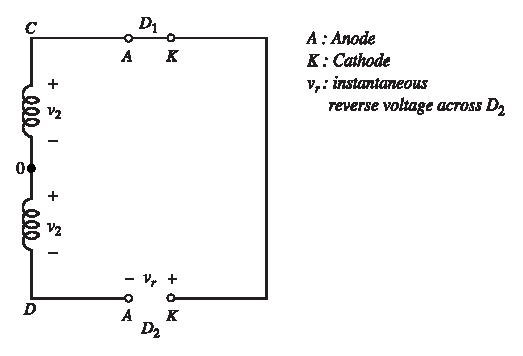
\includegraphics{chap2/add-fig/S3-EE-02-007.eps}
\caption{Equivalent circuit to find PIV}\label{fig2.7}
\end{figure}

\eject

Applying Kirchhoff's Voltage Law to the circuit of Fig. 2.7 we have,
\begin{align*}
v_2 + v_2 - v_r & = 0. \text{~~ But~~} v_2 = V_m \sin \omega t\\
v_r & = 2 v_2 = 2 V_m \sin \omega t\\
PIV & = v_{r \max} = 2 V_m, \quad \text{ when } \sin \omega t =1.
\end{align*}

{\em Therefore the peak inverse voltage in a full-wave rectifier with
centre tapped transformer is twice the peak secondary voltage of
transformer.}

\section{Summary of results for Full-wave rectifier using two diodes}\label{sec2.15}

The results obtained for full-wave rectifier using two diodes are
summarised in Table~\ref{tab2.2}.
\begin{table}[H]
\centering
\caption{Summary of results for full-wave rectifier with two diodes}\label{tab2.2}
\renewcommand{\arraystretch}{1.8}
\begin{tabular}{|c|c|c|}
\hline
\multirow{2}{1.5cm}{Parameter}\index{Full-wave rectifier!parameters} & \multicolumn{2}{c|}{Expression}\\\cline{2-3}
& Practical diode & Ideal diode $(R_f=0)$\\
\hline
Peak load\,/\,diode current $I_m$ & $\dfrac{V_m}{R_f + R_L}$ &
$\dfrac{V_m}{R_L}$\\[5pt]
\hline
DC load current \ $I_{dc}$ & $\dfrac{2V_m/\pi}{R_f + R_L} = \dfrac{2
  I_m}{\pi}$ & $\dfrac{2V_m/\pi}{R_L}$\\[5pt]
\hline
RMS load current \ $I_{rms}$ & $\dfrac{V_m/\sqrt{2}}{R_f +R_L} =
\dfrac{I_m}{\sqrt{2}}$ & $\dfrac{V_m/\sqrt{2}}{R_L}$\\[5pt]
\hline
DC load voltage \ $V_{dc}$ & $\dfrac{2V_m/\pi}{1+ R_f/R_L}$ & $2
V_m/\pi$\\[5pt]
\hline
RMS load voltage \ $V_{rms}$ & $\dfrac{V_m/\sqrt{2}}{1+ R_f / R_L}$ &
$V_m/\sqrt{2}$\\[5pt]
\hline
\% regulation & $\dfrac{R_f}{R_L} \times 100$ & 0\\[5pt]
\hline
Rectification efficiency \ $\eta_r$ & $\dfrac{0.812}{1 +R_f /R_L}$ &
0.812 or 81.2 \%\\[5pt]
\hline
Ripple factor \ $\gamma$ & 0.483 & 0.483\\
\hline
Peak inverse voltage \ PIV & $2 V_m$ & $2 V_m$\\
\hline
\end{tabular}
\end{table}

\eject

\begin{example}\label{exam2.6}
A full-wave single-phase rectifier consists of two diodes each having
internal resistance of 500 $\Omega$. The circuit feeds a pure resistive
load of 2000 $\Omega$. The secondary voltage with reference to centre
tap is 280 V. Calculate,
\begin{itemize}
\item[(a)] peak load current

\item[(b)] DC load current

\item[(c)] direct current in each diode 

\item[(d)] dc output power

\item[(e)] the percentage regulation

\item[(f)] PIV across each diode

\item[(g)] rms load current

\item[(h)] rms current through each diode 

\item[(i)] DC load voltage.
\end{itemize}
\end{example}

\begin{solution}
Given, 
\begin{align*}
R_f & = 500 \Omega\\
R_L & = 2000 \Omega
\end{align*}

Secondary voltage with reference to centre tap
\begin{align*}
V_2 & = 280 V \ \text{(RMS)}\\
V_{m}& = \sqrt{2}\, V_2=\sqrt{2}\times 280\text{\,V} \\
& = 395.98\, V
\end{align*}
\begin{figure}[H]
\centering
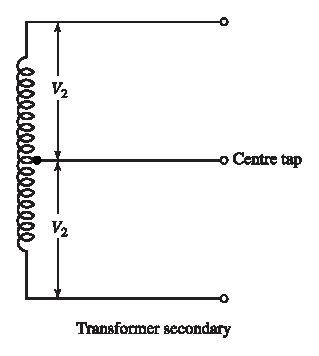
\includegraphics{chap2/add-fig/S3-EE-02-IN002.eps}
\end{figure}

\begin{itemize}
\item[(a)] Peak load current,
\begin{align*}
I_m & = \frac{V_m}{R_f + R_L}\\[4pt]
& = \frac{395.98 \V}{500\, \Omega + 2000\, \Omega}\\[3pt]
& = 158.39 \mA
\end{align*}


Note that peak load current is same as peak diode current.

\item[(b)] DC load current, 
\begin{align*}
I_{dc} & = \frac{2I_m}{\pi}\\
& = \frac{2}{\pi}\; [158.39\mA]= 100.83 \mA
\end{align*}

\item[(c)] Since each diode acts as a half-wave rectifier, the $dc$
  current through each diode is 
\begin{align*}
I_{dc(\text{diode})} & = I_m/\pi\\
& = 50.42 \mA
\end{align*}

\item[(d)] $dc$ output power,
\begin{align*}
P_{dc} & = [I_{dc}]^2 R_L\\
& = [100.83\,\mA]^2 [2000\,\Omega]\\
& = 20.33 \W.
\end{align*}

\item[(e)]
\begin{align*}
\% \ \text{regulation } & = \frac{R_f}{R_L} \times 100\\[4pt]
& = \frac{500\,\Omega}{2000\,\Omega} \times 100\\[4pt]
& = 25
\end{align*}

\item[(f)] PIV across each diode
\begin{align*}
& = 2 V_m = 2 \times 395.98 \V\\
& = 791.96 \V
\end{align*}

\item[(g)] RMS load current, 
\begin{align*}
I_{rms} & = \frac{I_m}{\sqrt{2}} = \frac{158.39 \mA}{\sqrt{2}}\\
& = 112 \mA
\end{align*}

\item[(h)] Since each diode acts as a half-wave rectifier, the RMS
  current through each diode is,
\begin{align*}
I_{rms\text{(diode)}} & = \frac{I_m}{2} = \frac{158.39\text{\,mA}}{2}\\
& = 79.195 \mA
\end{align*}

\item[(i)] DC load voltage,
\begin{align*}
V_{dc} & = I_{dc}\, R_L \\
& = [100.83 \mA] [2000\,\Omega]\\
& = 201.66 \V
\end{align*}
\end{itemize}
\vskip -.9cm
\end{solution}

\begin{example}\label{exam2.7}
In a two diode Fullwave rectifier circuit, the rms voltage across each
half of the transformer secondary is 100 V. The load resistance is
950 $\Omega$ and each diode has a forward resistance of 50
$\Omega$. Find the load current and rms value of the input current.
\end{example}

\begin{solution}
RMS voltage across each half of the transformer secondary,
\begin{align*}
V_2 & = 100 \V\\
\therefore\quad V_m & = \sqrt{2}\, V_2 = \sqrt{2}\times 100\text{\,V}=141.42\text{\,V}\\
R_f & = 50\, \Omega\\
R_L & = 950\, \Omega
\end{align*}
\begin{figure}[H]
\centering
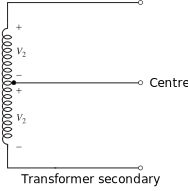
\includegraphics{chap2/add-fig/S3-EE-02-IN003.eps}
\end{figure}

Unless otherwise specified load current means DC load current.
\begin{align*}
I_{dc} & = 2 I_{m} /\pi\\
I_m & = \frac{V_m}{R_f + R_L}\\
& = \frac{141.42 \V}{50\,\Omega + 950\,\Omega}\\
& = 141.42 \mA \\
I_{dc} & = \frac{2}{\pi}\, [141.42 \mA] = 90 \mA
\end{align*}

RMS input current is same as RMS load current.
\begin{align*}
I_{rms} & = I_m / \sqrt{2}\; = \frac{141.42 \mA}{\sqrt{2}}\\
& = 100 \mA
\end{align*}
\vskip -.9cm
\end{solution}

\begin{example}\label{exam2.8}
A full-wave rectifier has a load of 2 K$\,\Omega$. The $ac$  voltage
applied to the diodes is 200\,V-0-200\,V. Assuming ideal diodes,
calculate
\begin{itemize}
\item[(a)] Average load current

\item[(b)] Average load voltage

\item[(c)] Ripple voltage

\item[(d)] What is the new value of the ripple voltage if a
  capacitor\footnote{The reader is adviced to solve part (d) only
    after going through Section \ref{sec2.21}.} of 500 $\mu F$ is connected  across
  the load. Take $f = 50$ Hz.
\end{itemize}
\end{example}

\begin{solution}
Given,
\begin{align*}
V_2 & = 200 \V\\
V_m & = \sqrt{2} V_2=\sqrt{2}\times 200\text{\,V}\\
& = 282.84 \V\\
R_L & = 2000 ~\Omega\\
R_f & = 0 \quad (\because \text{ ~ Diodes are ideal})\\
C & = 500 ~ \mu F, ~~~ f= 50 ~\Hz
\end{align*}
\begin{figure}[H]
\centering
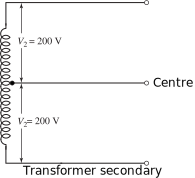
\includegraphics{chap2/add-fig/S3-EE-02-IN004.eps}
\end{figure}

\begin{itemize}
\item[(a)] Average load current,
\begin{align*}
I_{dc} & = \frac{2I_m}{\pi}\\ 
I_m & = \frac{V_m}{R_f + R_L}\\
& = \frac{282.84 \V}{2000\,\Omega}\\
& = 141.42\text{\,mA}\\
I_{dc} & = \frac{2}{\pi} [141.42 \mA] = 90 \mA\\
\end{align*}

\item[(b)] Average load voltage
\begin{align*}
V_{dc} & = I_{dc}\,R_L\\
& = (90 \mA) (2000 \Omega) = 180 V
\end{align*}

\item[(c)] Ripple factor,
\begin{align*}
\gamma & = \frac{V_{ac}}{V_{dc}}\\
\text{For FWR, } ~~ \gamma & = 0.483
\end{align*}

$\therefore$ RMS value of ripple voltage,
\begin{align*}
V_{ac} & = \gamma V_{dc}\\
& = (0.483) (180 \V)\\
& = 89.94 \V
\end{align*}

\item[(d)] With capacitor connected across $R_L$
\begin{align*}
\gamma & = \frac{1}{4\sqrt{3} f R_L C} \quad [\text{Refer equation \eqref{eq2.55}}]\\
& = \frac{1}{4\sqrt{3} (50) (2000) (500 \times 10^{-6})}\\
& = 2.89 \times 10^{-3}
\end{align*}
With capacitor filter,
\begin{align*}
V_{dc} & \simeq V_m \quad \text{[refer equation \eqref{eq2.65}]}\\
\text{But }  ~~~ V_{dc} & = 282.84 \V\\
\text{Now, } ~~~ V_{ac}& = \gamma V_{dc} \\
& = 0.8174 \V
\end{align*}
\end{itemize}
Note that when $C$ is connected across $R_L$, the ripple voltage
drastically reduces from 89.94 V to 0.8174 V.
\end{solution}

\begin{example}\label{exam2.9}
In a full-wave rectifier the input is from a 30\,V-0-30\,V transformer:
The load and diode forward resistances are 100 $\Omega$ and 10
$\Omega$ respectively. Calculate the average voltage, rectification
efficiency and percentage regulation.
\end{example}

\begin{solution}
RMS secondary voltage,
\begin{align*}
V_2 & = 30 \V\\
V_m & = \sqrt{2}\, \text{V}_2 = \sqrt{2}\times 30\text{\,V}=42.43\text{\,V}\\
R_L & = 100\,\Omega, ~~ R_f = 10\,\Omega
\end{align*}
\begin{figure}[H]
\centering
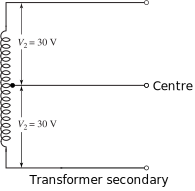
\includegraphics{chap2/add-fig/S3-EE-02-IN005.eps}
\end{figure}

\eject

~\phantom{a}
\vskip -.9cm

\begin{align*}
\text{Average output voltage,  } V_{dc} & = \dfrac{\frac{2V_m}{\pi}}{1
  + \frac{R_f}{R_L}}\\[4pt]
& = \frac{\left[\frac{2}{\pi} \times 42.43 \V \right]}{1 + \frac{10\,
    \Omega}{100\,\Omega}}\\[4pt]
 &= 24.56 \V\\[4pt]
\text{Rectification efficiency, $\eta_r$} & = \frac{0.812}{1 +
  \frac{R_f}{R_L}}\\[4pt]
& = \frac{0.812}{1+ \frac{10\,\Omega}{100\,\Omega}}\\[4pt]
& = 0.7382 \text{ ~ or  ~ } 73.82 \%\\[4pt]
\text{Percentage regulation } & = \frac{R_f}{R_L} \times 100\\[4pt]
& = \frac{10\,\Omega}{100\,\Omega} \times 100= 10
\end{align*}
\vskip -.9cm
\end{solution}

\smallskip
\begin{example}\label{exam2.10}
A full-wave rectifier using two diodes is supplied from an $ac$ supply
given by 220 sin 314t V through a centre-tapped transformer of turns
ratio 10:1. The load resistance is 1000 $\Omega$ and the diode forward
resistance is 20 $\Omega$.

\noindent
Calculate
\begin{itemize}
\itemsep=1pt
\item[(a)] Average load voltage

\item[(b)] RMS load current

\item[(c)] PIV across each diode 

\item[(d)] DC output power and

\item[(e)] Frequency of output waveform
\end{itemize}
\end{example}

\begin{solution}
Given,
\begin{align*}
v_1 & = 220 ~~ \sin 314 t\V\\
\frac{N_1}{N_2} & = 10\\
\frac{v_1}{v_2} & = \frac{N_1 }{N_2}\\[4pt]
v_2 & = \frac{N_2}{N_1} v_1 = \frac{1}{10} \ \ [220 \sin 314 t \V]\\[4pt]
& = 22 \sin 314 t \V = V_m \sin \omega\, t \\[4pt]
\text{Comparing, we get } ~~ V_{m} & = 22 \V \\[4pt]
\omega & = 314\, r/s\\[4pt]
R_f & = 20\, \Omega \quad R_L = 1000\,\Omega\\[4pt]
\omega & = 2 \pi f\\[4pt]
f & = \omega/ 2 \pi = 50 \Hz
\end{align*}
\begin{figure}[H]
\centering
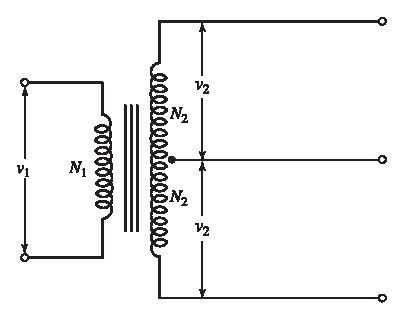
\includegraphics{chap2/add-fig/S3-EE-02-IN006.eps}
\end{figure}

\begin{itemize}
\item[(a)] Average load voltage
\begin{align*}
V_{dc} & = \frac{2V_m/\pi}{1 + R_f / R_L}\\[4pt]
& = \frac{(2/\pi) (22 \V)}{1+ \left(\frac{20\,\Omega}{1000\,\Omega}
  \right)}\\[4pt]
& = 13.73 \V
\end{align*}

\item[(b)] RMS load current
\begin{align*}
I_{rms} & = \frac{I_m}{\sqrt{2}}\\[4pt]
I_m & = \frac{V_m}{R_f + R_L}\\[4pt]
&= \frac{22\V}{20\,\Omega + 1000\,\Omega}= 21.57 \mA\\[3pt]
I_{rms} & = \frac{I_m}{\sqrt{2}} = 15.25 \mA
\end{align*}

\eject

\item[(c)] \hfill \text{PIV across each diode ~}  $= 2 V_m = 44 \V$\hfill\,

\item[(d)] $dc$ output power
\begin{align*}
P_{dc} & = V_{dc}\, I_{dc} = \frac{V^2_{dc}}{R_L}\\[4pt]
& = \frac{(13.73 \V)^2}{1000\,\Omega}\\[4pt]
& = 0.1885 \W
\end{align*}

\item[(e)] For one cycle of $ac$ input, the rectified output contains
  two cycles. Hence, the frequency of output waveform is twice the
  frequency of $ac$ input.
$$
\therefore ~~ \text{ Frequency of output waveform = $2\,(50\,\text{Hz})= 100 \Hz$}
$$
\end{itemize}
\vskip -1cm
\end{solution}

\section{Full-wave bridge rectifier}\label{sec2.16}
\begin{figure}[H]
\centering
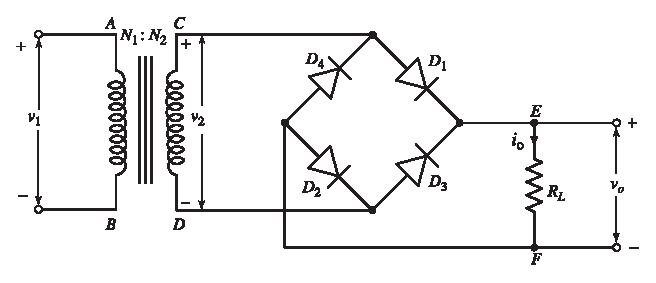
\includegraphics{chap2/add-fig/S3-EE-02-008.eps}
\caption{Full-wave bridge rectifier}\label{fig2.8}
\end{figure}

Fig.~\ref{fig2.8} shows the circuit of a full-wave bridge rectifier.\index{Bridge rectifier}\index{Rectifier!bridge rectifier} It uses
four diodes which are arranged in the form of a bridge and a
transformer without centre tapping.

Instantaneous primary voltage, $v_1 = V_m \sin \omega t$.

Instantaneous secondary voltage,
$$
v_2 = (N_2/N_1) v_1 = (N_2 / N_1) V_m \sin \omega t
$$

During the positive half-cycle of $ac$ supply, the voltage at point
C is positive-going with respect to point $D$. Diodes $D_1$ and $D_2$
are forward biased and $D_3$ and $D_4$ are reverse biased. The current
follows the path $C-D_1-E-F-D_2-D-C$. During this interval, $i_o
=i_{d_1} = i_{d_2}$.

During the negative half-cycle of $ac$ supply, the voltage at point
$D$ is positive-going with respect to point $C$. Diodes $D_3$ and
$D_4$ are forward biased and $D_1$ and $D_2$ are reverse biased. The
current follows the path $D-D_3 - E- F-D_4 - C-D$. During this
interval, $i_o= i_{d_3} = i_{d_4}$.

Note that during both half-cycles of $ac$ supply load current $i_o$
flows from $E$ to $F$. Hence $i_o$ is unidirectional. The various
voltage and current waveforms\index{Bridge rectifier!waveforms} are shown in Fig.~\ref{fig2.9}.

\begin{example}\label{exam2.11}
For a Full-wave bridge rectifier, obtain the expressions for the
following
\begin{itemize}
\item[(a)] $I_{dc}$ and $V_{dc}$

\item[(b)] $I_{rms}$ and $V_{rms}$

\item[(c)] percentage regulation

\item[(d)] Rectification efficiency and

\item[(e)] ripple factor
\end{itemize}
\end{example}

\begin{solution}
Let us write the equivalent circuit when $D_1$ and $D_2$ are
conducting and $D_3$ and $D_4$ are not conducting, from the circuit of
Fig.~\ref{fig2.8}. $D_1$ and $D_2$ are replaced by $R_f$ and $D_3$ and $D_4$
are represented by open circuits in the equivalent circuit\index{Bridge rectifier!equivalent circuit} shown in
Fig.~\ref{fig2.10}.

Applying Kirchhoff's Voltage Law to the circuit of Fig.~\ref{fig2.10} we get
\begin{align}
v_2 - i_0\, R_f - i_0\, R_L - i_0\, R_f & =0 \notag\\
i_0 & = \frac{v_2}{2 R_f + R_L} \label{eq2.42}
\end{align}

But \  $v_2 = (N_2/N_1) \ v_1 = (N_2/N_1) V_m \sin \omega t$. Taking $N_1 /
N_2 =1$, we have
$$
v_2 = V_m \sin \omega t
$$

Using this relation in equation \eqref{eq2.42} we get
\begin{align}
i_0 & = \frac{V_m}{2 R_f + R_L} \sin \omega t  \notag\\
& = I_m \sin \omega t, \quad 0 \leq \omega t \leq \pi \label{eq2.43}\\
\text{where } \quad I_m & = \frac{V_m}{2 R_f + R_L} \label{eq2.44}
\end{align}

During the negative-half cycle of $v_2$, diodes $D_3$ and $D_4$
conduct and $D_1$ and $D_2$ are reverse biased. By comparing equations
\eqref{eq2.44} and \eqref{eq2.26} we note that, equation
\eqref{eq2.44} can be obtained from equation \eqref{eq2.26} by
replacing $R_f$ by $2 R_f$.


The results obtained in sections \ref{sec2.10}, \ref{sec2.11}, \ref{sec2.12} and \ref{fig2.13} for two diode
circuit can be extended for bridge rectifier by replacing $R_f$ by $2
R_f$. The results are summarised in Table~\ref{tab2.3}.
\begin{figure}[H]
\centering
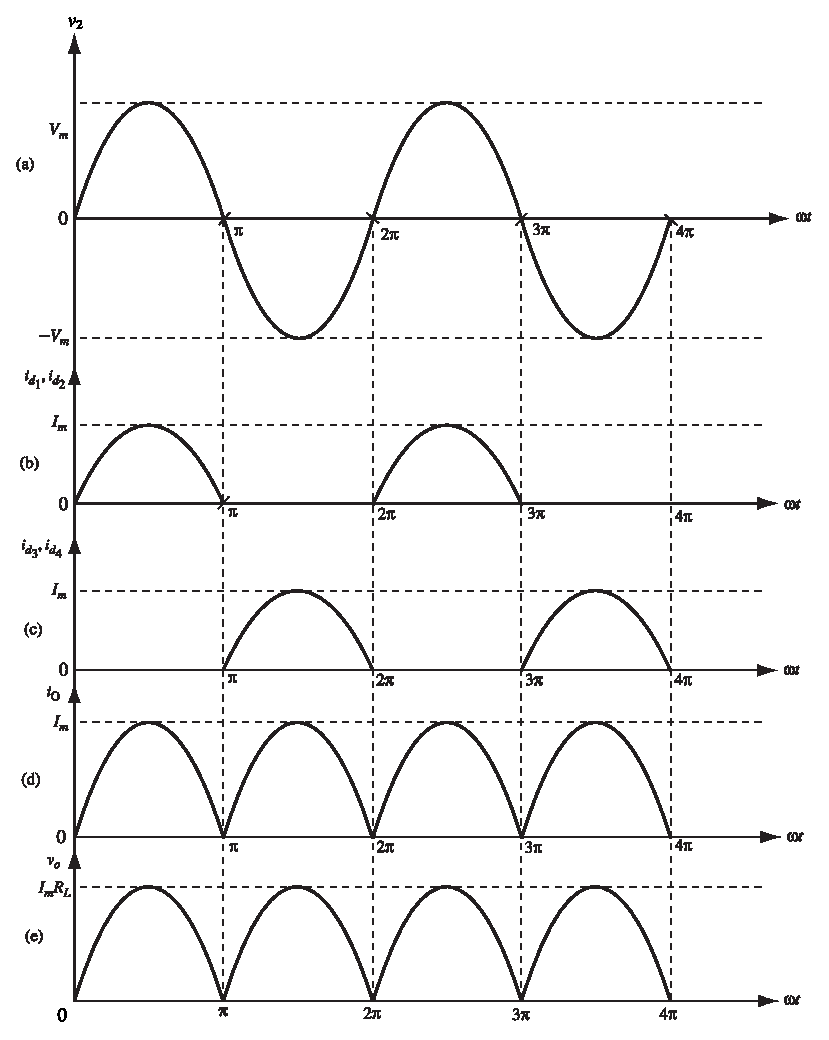
\includegraphics{chap2/add-fig/S3-EE-02-009.eps}
\caption{Voltage and current waveforms in full-wave bridge rectifier}\label{fig2.9}
\end{figure}

\begin{figure}[H]
\centering
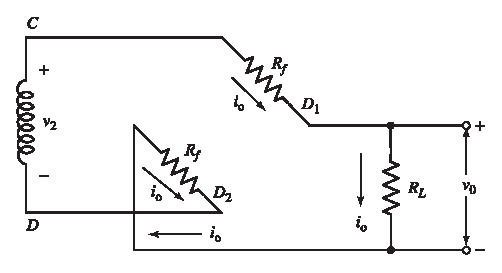
\includegraphics{chap2/add-fig/S3-EE-02-010.eps}
\caption{Equivalent circuit of bridge rectifier during positive half-cycle of $ac$ input}\label{fig2.10}
\end{figure}

\begin{table}[H]
\centering
\renewcommand{\arraystretch}{1.8}
\tabcolsep=12pt
\caption{Summary of results for full-wave Bridge rectifier}\label{tab2.3}
\begin{tabular}{|c|c|c|}
\hline
\multirow{2}{1.5cm}{Parameter}\index{Bridge rectifier!parameters} & \multicolumn{2}{c|}{Expression}\\\cline{2-3}
& Practical diode & Ideal diode $(R_f=0)$\\
\hline
Peak load or diode current, $I_m$ & $\dfrac{V_m}{2 R_f + R_L}$ &
$\dfrac{V_m}{R_L}$\\[5pt]
\hline
DC load current, $I_{dc}$ & $\dfrac{2 V_m/\pi}{2 R_f + R_L} = \dfrac{2
I_m}{\pi}$ & $\dfrac{2 V_m/\pi}{R_L}$\\[5pt]
\hline
RMS load current, $I_{rms}$ & $\dfrac{V_m/\sqrt{2}}{2 R_f + R_L} =
\dfrac{I_m}{\sqrt{2}}$ & $\dfrac{V_m/\sqrt{2}}{R_L}$\\[5pt]
\hline
DC load voltage, $V_{dc}$ & $\dfrac{2V_m/\pi}{1+2 (R_f /R_L)}$ & $2
V_m/\pi$\\[5pt]
\hline
RMS load voltage, $V_{rms}$ & $\dfrac{V_m/\sqrt{2}}{1+ 2 (R_f /R_L)}$ &
$V_m/\sqrt{2}$\\[5pt]
\hline
\% \text{ regulation} & $\dfrac{2 R_f}{R_L} \times 100$ & 0\\[5pt]
\hline
Rectification efficiency, $\eta_r$ & $\dfrac{0.812}{1+ 2 (R_f /R_L)}$ &
0.812 or 81.2 \%\\[5pt]
\hline
Ripple factor, $\gamma$ & 0.483 & 0.483\\
\hline
Peak Inverse Voltage PIV & \multicolumn{2}{c|}{$V_m$ (Refer section
  \ref{sec2.17})}\\
\hline
\end{tabular}
\end{table}

\medskip
\noindent{\textbf{Note:}} The reader is adviced to repeat Example
\eqref{eq2.5} for full-wave bridge rectifier and obtain $R_L = 2 R_f$
as the condition for maximum power transfer from the rectifier to the load.
\end{solution}

\section{Peak inverse voltage for full-wave bridge
  rectifier}\label{sec2.17}
\index{Bridge rectifier!peak inverse voltage}
 
Let us write the equivalent circuit of a full-wave bridge rectifier
when $D_1$ and $D_2$ are conducting and $D_3$ and $D_4$ are not
conducting, using the circuit of Fig.~\ref{fig2.8}.

The conducting diodes are replaced by short circuits and the non-conducting diodes by open circuits as shown in the equivalent circuit of Fig.~\ref{fig2.11}.
\begin{figure}[H]
\centering
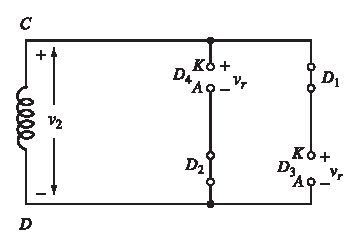
\includegraphics{chap2/add-fig/S3-EE-02-011.eps}
\caption{Equivalent circuit to find PIV, for bridge rectifier}\label{fig2.11}
\end{figure}

Diodes $D_4$ and $D_3$ are in parallel and they are connected between
the secondary of the transformer. Writing Kirchhoff's Voltage Law to
the first loop we have,
\begin{align*}
v_2 - v_r & = 0\\
v_r & = v_2 = V_m \sin \omega t\\
\text{PIV } & = v_{r \max} = V_m
\end{align*}

\begin{example}\label{exam2.12}
In a full-wave bridge rectifier, the transformer secondary voltage is
$100 \sin \omega t \V$. The forward resistance of each diode is 25
$\Omega$ and the load resistance is 950 $\Omega$. Calculate
\begin{itemize}
\itemsep=1pt
\item[(a)] $dc$ output voltage

\item[(b)] Ripple factor

\item[(c)] Efficiency of rectification

\item[(d)] PIV across non-conducting diode 

\item[(e)] Percentage regulation

\item[(f)] Peak diode current

\item[(g)] dc load current

\item[(h)] dc current through each diode

\item[(i)] RMS current through each diode
\end{itemize}
\end{example}

\begin{solution}
Given, 
\begin{align*}
v_2 & = 100 \sin \omega t \V = V_m \sin \omega t\\
\therefore\quad V_m & = 100 \V\\
R_f & = 25 \Omega\\
R_L & = 950\, \Omega
\end{align*}
\begin{itemize}
\item[(a)] $dc$ output voltage 
\begin{align*}
V_{dc} &= \frac{2V_m/\pi}{1 + (2 R_f /R_L)}\\
& = \frac{(2/\pi) (100 V)}{1 + 2 (25\, \Omega / 950\, \Omega)}\\
& = 60.48 \V.
\end{align*}
 
\item[(b)] Ripple factor 
\begin{align*}
\gamma &  = \sqrt{(V_{rms} / V_{dc})^2  -1}\\
V_{rms}& = \frac{V_m /\sqrt{2}}{1 + (2 R_f / R_L)}\\
& = \frac{(100 V/\sqrt{2})}{1 + 2 [25\,\Omega /950\,\Omega]}\\
& = 67.10 \V\\
\gamma & = \sqrt{(67.10/60.48)^2 -1}\\
& = 0.484
\end{align*}
 
\item[(c)] Efficiency of rectification
\begin{align*}
\eta_r & = \frac{0.812}{1+2 (R_f / R_L)}\\
& = \frac{0.812}{1+2 (25 \,\Omega / 950\, \Omega)}\\
& = 0.7714 \text{ or } 77.14 \% 
\end{align*}
 
\item[(d)] PIV across the non-conducting diode 
\begin{align*}
& = V_m\\
& = 100 \V.
\end{align*}

\item[(e)] Percentage regulation
\begin{align*}
& = \frac{2 R_f}{R_L} \times 100\\
& = \frac{2(25\,\Omega)}{950\,\Omega} \times 100\\
& = 5.26\,\%
\end{align*}

\item[(f)] Peak load current\,/\,peak diode current
\begin{align*}
I_m & = \frac{V_m}{2 R_f + R_L}\\
& = \frac{100\,\Omega}{2(25\,\Omega) + 950\,\Omega }\\
& = 100 \mA
\end{align*}

\item[(g)] DC load current
\begin{align*}
I_{dc} & = \frac{2I_m}{\pi}\\
& = \frac{2}{\pi}\, (100 \mA)\\
& = 63.66 \mA
\end{align*}

\item[(h)] Each diode acts as a half-wave rectifier.

$\therefore$ ~ $dc$ current through each diode,
\begin{align*}
I_{dc (\text{diode})} & = \frac{I_{dc}}{2} = \frac{63.66 \mA}{2}\\
& = 31.83 \mA
\end{align*}

\item[(i)] RMS current through each diode, 
\begin{align*}
I_{rms (\text{diode})} & = \frac{I_m}{2} = \frac{100\mA}{2}\\
& = 50 \mA
\end{align*}
\end{itemize}
\vskip -1cm
\end{solution}

\begin{example}\label{exam2.13}
A bridge rectifier is driving a load resistance of 100 $\Omega$. It is
driven by a source voltage of 230 V, 50~Hz. Neglecting diode
resistances, calculate
\begin{itemize}
\item[(a)] average output voltage

\item[(b)] average load current

\item[(c)] frequency of output waveform

\item[(d)] $dc$ power output.
\end{itemize}
\end{example}

\begin{solution}
Given,
\begin{align*}
V_2 & = 100 \V.\\
V_m & = \sqrt{2}\, V_2=\sqrt{2}\times 100\text{\,V}\\
& = 141.42 \V\\
R_f & = 0\\
R_L & = 100 \Omega\\
f & = 50 \Hz
\end{align*}

\begin{itemize}
\item[(a)] Average output voltage, 
\begin{align*}
V_{dc} & = \frac{\left(\frac{2 V_m}{\pi} \right)}{1 +2 R_f / R_L}
\\
& = \frac{2\,(\frac{141.42 \V}{\pi})}{1+0}\\
& = 90.03 \V.
\end{align*}

\item[(b)] Average load current,
\begin{align*}
I_{dc} & = \frac{V_{dc}}{R_L}\\
& = \frac{90 V}{100\, \Omega} \\
& = 0.9\text{\,A}
\end{align*}

\item[(c)] For one cycle of $ac$ input, the rectifier output contains
  two cycles. Therefore the frequency of output waveform is twice the
  frequency of $ac$ input.

Frequency of output waveform $=2(50\Hz) = 100 \Hz$.

\item[(d)] $dc$ power output.
\begin{align*}
P_{dc} & = (I_{dc})^2 R_L = (0.9 A)^2 (100\, \Omega)\\
& = 81 \W.
\end{align*}
\end{itemize}

\subsection{Comparative study of rectifier circuits}\label{sec2.17.1}

The comparative study of all rectifier circuits is shown in Table~\ref{tab2.4}.
\begin{table}[H]
\centering
\renewcommand{\arraystretch}{1.7}
\tabcolsep=2.5pt
\caption{Comparative study of all rectifier circuits}\label{tab2.4}
\begin{tabular}{|l|c|c|c|}
\hline
& & \multicolumn{2}{c|}{{\bf Full-wave rectifier}}\\\hline
\multicolumn{1}{|c|}{\bf Parameter} & {\bf Half-wave rectifier} & {\bf Two diode circuit}
& {\bf Four diode circuit}\\
\hline
Number of diodes & One & Two & Four\\
\hline
Transformer requirement & Transformer without & Transformer with &
Transformer without \\[-0.3cm]
& centre tapping & center tapping & centre tapping \\
\hline
Transformer utility & Poor & Poor & Better\\
\hline
PIV across each diode & $V_m$ & 2 $V_m$ & $V_m$ \\
\hline
Ripple factor, $\gamma$ & 1.21 & 0.483 & 0.483\\
\hline
Rectification efficiency, $\eta_r$ & $\frac{40.6}{1+\frac{R_f}{R_L}}\%$
& $\frac{81.2}{1+\frac{R_f}{R_L}} \%$ &
$\frac{81.2}{1+\frac{2R_f}{R_L}} \%$ \\[5pt]
& Ideal: 40.6\% & Ideal: 81.2 \% & Ideal: 81.2 \%\\
\hline
\% Regulation & $\frac{R_f}{R_L} \times 100$ & $\frac{R_f}{R_L}
\times 100$ & $\frac{2R_f}{R_L} \times 100$\\[5pt]
\hline
DC output voltage, $V_{dc}$ & $\frac{V_m/\pi}{1+ (R_f/R_L)}$ &
$\frac{2V_m/\pi}{1+ (R_f /R_L)}$ & $\frac{2V_m/\pi}{1+ (2R_f /R_L)}$\\[5pt]
& Ideal: $V_m /\pi$ & Ideal: $2V_m/\pi$ & Ideal: $2 V_m/ \pi$\\
\hline
RMS output voltage, $V_{rms}$ & $\frac{V_m/2}{1 + (R_f /R_L)}$ &
$\frac{V_m\sqrt{2}}{1+ (R_f/R_L)}$ & $\frac{V_m/ \sqrt{2}}{1+ (2 R_f /
  R_L)}$\\[5pt]
& Ideal: $V_m/2$ & Ideal: $V_m/\sqrt{2}$ & Ideal: $V_m/\sqrt{2}$\\
\hline
DC output current, $I_{dc}$ & $I_m/\pi ~:~ I_m = \frac{V_m}{R_f + R_L}$
& $2 I_m/\pi ~:~ I_m = \frac{V_m}{R_f + R_L}$ & $2 I_m/\pi ~:~ I_m =
\frac{V_m}{2 R_f + R_L}$\\[5pt]
\hline
RMS output current & $\dfrac{I_m}{2}$ & $\dfrac{I_m}{\sqrt{2}}$ &
$\dfrac{I_m}{\sqrt{2}}$\\[5pt]
\hline
\end{tabular}
\end{table}
\vskip -.8cm
\end{solution}

\section{Filters for rectifier circuits}\label{sec2.18}
\index{Rectifier!filters}

Filter is a circuit  used to reduce the ripple content present in the
rectified output. The ripple content of rectified output can be
filtered out by connecting a capacitor in parallel with $R_L$.

The output from full-wave and half-wave rectifiers is not a smooth
$dc$ due to the ripple content. The ripple content of half-wave
rectified output is 121\% of $dc$ component whereas it is 48.3\% of
$dc$ component in full-wave rectified output. In order to obtain
smooth $dc$, it is  necessary to filter out the ripple content.

\section{Half-wave rectifier with capacitor filter}\label{sec2.19}
\index{Half-wave rectifier!capacitor filter}
\begin{figure}[H]
\centering
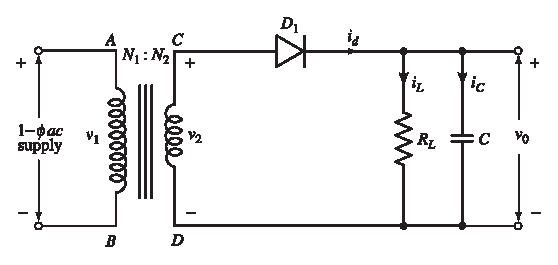
\includegraphics{chap2/add-fig/S3-EE-02-012.eps}
\caption{Half-wave rectifier with capacitor filter}\label{fig2.12}
\end{figure}

Fig.~\ref{fig2.12} shows the circuit of a half-wave rectifier with capacitor
filter. Fig.~\ref{fig2.13} shows the output voltage waveform with and without
capacitor filter. The following notations are used.
\begin{tabbing}
$V_{r(p-p)}$ is peak-peak ripple voltage on capacitor\\[3pt]
$t_c$ is charging time of capacitor\\[3pt]
$t_d$ is discharge time of capacitor.\\[3pt]
$T = t_c + t_d$ is the time period of output waveform.
\end{tabbing}

During the positive half-cycle of the $ac$ supply, the diode conducts
and charges the capacitor to the peak value $V_m$ of the transformer
secondary voltage. When the transformer secondary voltage falls below
$V_m$, the diode stops conducting.

Now, the capacitor starts discharging into 
$R_L$ and the voltage on capacitor decreases. The discharging of the
capacitor continues untill the diode  starts conducting again and
charges the capacitor in the next positive half-cycle of $ac$ supply.

From the waveforms shown in Fig.~\ref{fig2.13}, we find that without filter
capacitor, $v_0$ varies between zero and $V_m$ and with capacitor
filter, the variation is between $[V_m - V_{r(p-p)}]$ and $V_{m}$.
\begin{figure}[H]
\centering
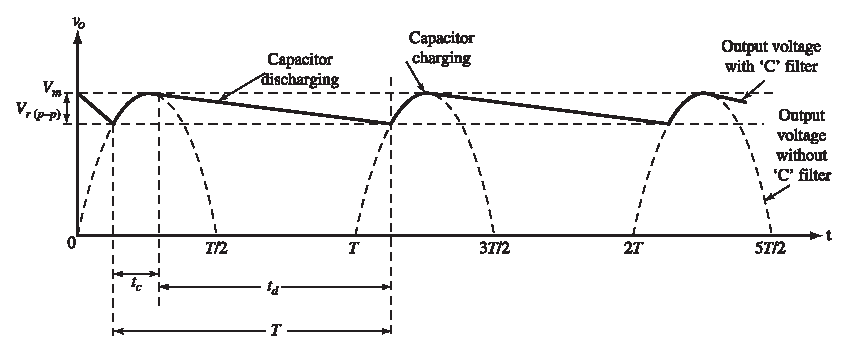
\includegraphics[scale=.93]{chap2/add-fig/S3-EE-02-013.eps}
\caption{Output voltage waveforms with and without `C' filter}\label{fig2.13}
\end{figure}

Note that with filter, the variation in $v_0$ is smaller than that of 
without filter. This clearly indicates that the shunting of $R_L$ by
$C$ considerably reduces the ripple content of the output voltage.
The ripple factor with `$C$' filter is give by 
$$
\gamma = \frac{1}{2 \sqrt{3} f R_L C}
$$

From the above equation we find that, $\gamma$ can be kept small by
using a large value of filter capacitor.

\section{Expressions for ripple factor and $dc$ output voltage in half
wave rectifier with capacitor filter}\label{sec2.20}
\index{Ripple factor!with capacitor filter}

The ripple factor, $\gamma$ is defined by
\begin{equation}
\gamma = \frac{V_{ac}}{V_{dc}} \label{eq2.45}
\end{equation}

$V_{ac}$ is the rms value of ripple voltage on capacitor

$V_{dc}$ is the $dc$ output voltage.

When the filter capacitor is large, the ripple voltage shown in
Fig.~\ref{fig2.13} can be approximated by a triangular waveform with a peak to
peak value $V_{r\,(p-p)}$, as shown in Fig.~\ref{fig2.14}.

For a triangular waveform with peak to peak value $V_{r\,(p-p)}$, the
rms value is given by
\begin{equation}
V_{ac} = \frac{V_{r\,(p-p)}}{2 \sqrt{3}} \label{eq2.46}
\end{equation}
\begin{figure}[H]
\centering
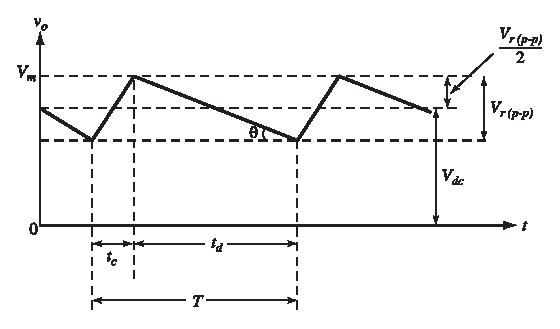
\includegraphics{chap2/add-fig/S3-EE-02-014.eps}
\caption{Ripple voltage on capacitor approximated by triangular waveform}\label{fig2.14}
\end{figure}

During the period $t_d$, the capacitor discharges a steady current
into the load, i.e.
\begin{equation}
\text{i.e. } ~~ i_c = I_{dc} = C\, \frac{dv_0}{dt} \label{eq2.47}
\end{equation}

From Fig.~\ref{fig2.14}, \ $\dfrac{dv_0}{dt} =$ Slope of ripple voltage waveform
during discharge.
$$
\text{But,\quad Slope } = \tan \theta = \frac{V_{r\,(p-p)}}{t_d}
$$

Using this relation in equation \eqref{eq2.47}
\begin{align}
I_{dc} & = C\,\frac{V_{r\,(p-p)}}{t_d} \label{eq2.48}\\
V_{r\,(p-p)} & = \frac{I_{dc}\, t_d}{C} \label{eq2.49}\\
\text{Also, \ } \quad T & = t_c + t_d. \label{eq2.50} 
\end{align}

When $C$ is large, $t_c \ll t_d$.

From equation \eqref{eq2.50}, $t_d \simeq T = 1 /f$. Using this relation in
equation \eqref{eq2.49}, we have
\begin{align}
V_{r\,(p-p)} & = \frac{I_{dc}}{f C} \label{eq2.51}\\
\text{But } \quad I_{dc} & = V_{dc} / R_L \notag
\end{align}

Also from equation \eqref{eq2.46}, $V_{r(p-p)} = 2 \sqrt{3} V_{ac}$

Using these relations in equation \eqref{eq2.51}, we get
\begin{align}
2 \sqrt{3} V_{ac} & = \frac{V_{dc}}{f C R_L} \notag\\
\text{Now, } ~~ \gamma & = \frac{V_{ac}}{V_{dc}} = \frac{1}{2 \sqrt{3}f
C R_L} \label{eq2.52}
\end{align}

\heading{\boldmath$dc$ output voltage, $V_{dc}$}

The triangular waveform of peak to peak value $V_{r\,(p-p)}$ has an
average value of $\dfrac{V_{r\,(p-p)}}{2}$. Therefore, the $dc$ output
voltage
$$
V_{dc}  = V_m - \frac{V_{r\,(p-p)}}{2}
$$

Substituting for $V_{r\,(p-p)}$ from equation \eqref{eq2.51} we have
\begin{align}
V_{dc} & = V_m - \frac{1}{2} \left[\frac{I_{dc}}{f C} \right] \notag\\
V_{dc} & = V_m - I_{dc} \left[\frac{1}{2 fC} \right] \label{eq2.53}
\end{align}

From equation \eqref{eq2.53} we find that, when the filter capacitor
$C$ is large, $\dfrac{1}{2 fC}$ is small
\begin{equation}
\therefore \quad V_{dc} \simeq V_m \label{eq2.54}
\end{equation}

\begin{example}\label{exam2.14}
A half-wave rectifier with capacitor filter is supplying a resistive
load of 1000\,$\Omega$. The value of filter capacitor is 200 $\mu$\,F. If the supply voltage to the rectifier is \hbox{200\,V} at 50 Hz, calculate
\begin{itemize}
\itemsep=2pt
\item[(a)] Ripple factor

\item[(b)] $dc$ output voltage

\item[(c)] DC load current

\item[(d)] PIV across the diode 

\item[(e)] RMS ripple output voltage.
\end{itemize}
\end{example}

\eject

\begin{solution}
\begin{align*}
V_2 & = 220 \V, V_m = 220 \sqrt{2} = 311.13 \V.\\
f & = 50 \Hz \\
C & = 200\,\mu \F\\
R_L & = 1000\,\Omega
\end{align*}

\begin{itemize}
\item[(a)] Ripple factor,
\begin{align*}
\gamma &= \frac{1}{2 \sqrt{3} f R_L C}\\
& = \frac{1}{2 \sqrt{3} (50) (1000) (200 \times 10^{-6})}\\
& = 0.029 \text{~ or ~} 2.89\%
\end{align*}

\item[(b)] $dc$ output voltage,
\begin{align*}
V_{dc} & = V_m - I_{dc} \left[\frac{1}{2 f C} \right]\\
\text{But} \quad I_{dc} & = V_{dc}/R_L\\
\therefore ~ V_{dc} & = V_m - \frac{V_{dc}}{R_L} \left[\frac{1}{2 f C}
  \right]\\
V_{dc} & = \frac{V_m}{1 + \left[2 f C R_L \right]}\\
& = \frac{311.13\text{\,V}}{1 + \left[\frac{1}{2 (50) (200 \times 10^{-6})
      (1000)} \right]}\\
V_{dc} & = 296.31 \V
\end{align*} 

\item[(c)] DC load current,
\begin{align*}
I_{dc} & = \frac{V_{dc}}{R_L}\\
& = \frac{296.31\,\text{V}}{1000\,\Omega}\\
& = 0.296 \A
\end{align*}

\item[(d)] Peak inverse voltage,
\begin{align*}
\text{PIV} & = V_m\\
& = 311.13 \V
\end{align*}

\item[(e)] RMS ripple voltage on capacitor, $V_{ac}$
\begin{align*}
\gamma & = \frac{V_{ac}}{V_{dc}}\\
V_{ac} & = \gamma V_{dc}\\
& = (0.0289) (296.31\text{\,V})\\
& = 8.56 \V.
\end{align*}
\end{itemize}
\vskip -.9cm
\end{solution}

\begin{example}\label{exam2.15}
A half-wave rectifier with capacitor  filter is supplying a resistive
load of \hbox{500\,$\Omega$.} If the load ripple content should not exceed
10\%, find the value of capacitance required. The supply frequency is
50 Hz.
\end{example}

\begin{solution}
\begin{align*}
f & = 50 ~ \Hz\\[3pt]
R_L & = 500 ~ \Omega\\[3pt]
\% ~~ \gamma & < 10\\[3pt]
\gamma & < \dfrac{10}{100} \Rightarrow  \gamma < 0.1\\[3pt]
\gamma & = \frac{1}{2 \sqrt{3} f R_L C} < 0.1\\[3pt]
\text{or } \quad C & > \frac{1}{2 \sqrt{3} (0.1) (f) R_L}\\[3pt]
& >  \frac{1}{2 \sqrt{3} (0.1) (50) (500)}\\[3pt]
C & > 115.47 ~\mu\, \F 
\end{align*}
\vskip -.9cm
\end{solution}

\section{Full-wave rectifier with capacitor filter}\label{sec2.21}
\index{Full-wave rectifier!with capacitor filter}

Fig.~\ref{fig2.15} shows the circuit of a full-wave rectifier with capacitor
filter. Fig.~\ref{fig2.16} shows the output voltage waveforms with and without
capacitor filter.

$V_{r\,(p-p)}$ is the peak to peak ripple voltage on capacitor.

$t_c$ is the charging time of capacitor

$t_d$ is the discharge time of capacitor

Time period of output waveform, $\dfrac{T}{2} = t_c + t_d$.
\begin{figure}[H]
\centering
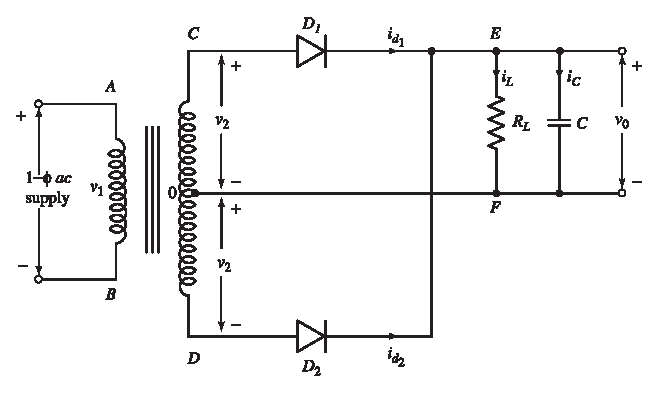
\includegraphics{chap2/add-fig/S3-EE-02-015.eps}
\caption{Full-wave rectifier with capacitor filter}\label{fig2.15}
\end{figure}

\begin{figure}[H]
\centering
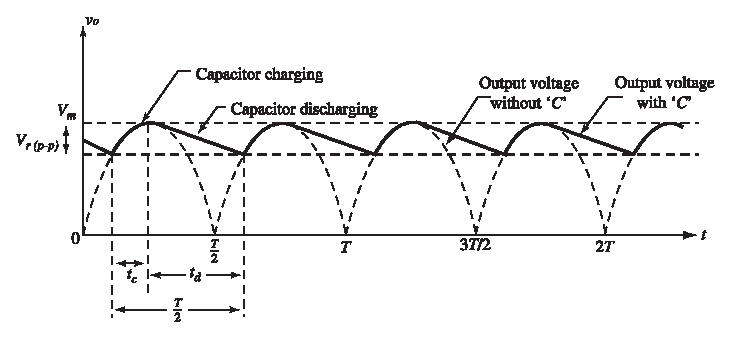
\includegraphics{chap2/add-fig/S3-EE-02-016.eps}
\caption{Output voltage waveforms with and without `C' filter}\label{fig2.16}
\end{figure}

During the positive half-cycle of the $ac$ supply, the diode $D_1$
conducts and charges the capacitor to the peak value $V_m$ of the
transformer secondary voltage. $D_1$ stops conducting when the
transformer secondary voltage falls below $V_m$.

Now, the capacitor starts discharging into $R_L$ and the voltage on
the capacitor begins to fall. The discharging of the capacitor
continues until the diode $D_2$ start conducting again in the next
cycle and charges the capacitor.

\eject

From the waveforms of Fig.~\ref{fig2.16}, we find that without filter
capacitor, $v_0$ varies between zero and $V_m$ and with filter the
variation is between $[V_m-V_{r(p-p)}]$ and $V_m$. Note that with
filter capacitor, the variation in $v_0$ is smaller than that without
filter capacitor. This clearly indicates that the shunting of $R_L$ by
$C$ considerably reduces the ripple content of output voltage. The
ripple factor with $C$ filter is given by
\begin{equation}
\gamma = \frac{1}{4 \sqrt{3} f R_L C}  \label{eq2.55}
\end{equation}

From the above equation we find that $\gamma$ can be made small by
using a large filter capacitor.

\section{Full-wave bridge rectifier with capacitor
  filter}\label{sec2.22}
\index{Bridge rectifier!capacitor filter}
\begin{figure}[H]
\centering
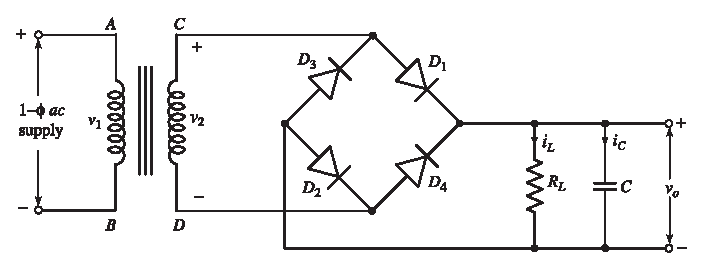
\includegraphics[scale=.95]{chap2/add-fig/S3-EE-02-017.eps}
\caption{Full-wave bridge rectifier with capacitor filter}\label{fig2.17}
\end{figure}

\begin{figure}[H]
\centering
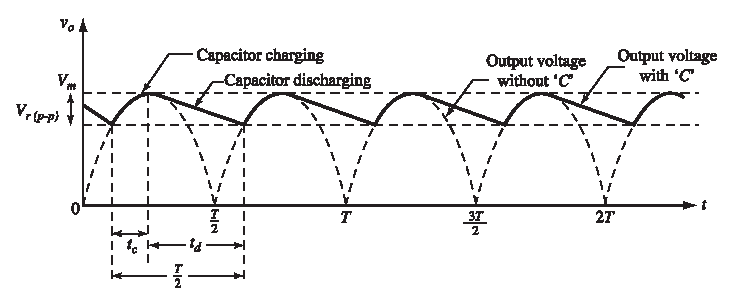
\includegraphics[scale=.95]{chap2/add-fig/S3-EE-02-018.eps}
\caption{Output voltage waveforms with and without `C' filter}\label{fig2.18}
\end{figure}
During the positive half-cycle of the $ac$ supply, diodes $D_1$ and
$D_2$ conduct and charge the capacitor to the peak value $V_m$ of the
transformer. Diodes $D_1$ and $D_2$ stop  conducting when the
transformer secondary voltage falls below $V_m$.

Now the capacitor starts discharging into $R_L$ and the voltage in the
capacitor begins to fall. The discharging of the capacitor continues
until the diode $D_3$ and $D_4$ start conducting and charge the
capacitor in the next half-cycle of the $ac$ supply. 

From the waveforms of Fig.~\ref{fig2.18} we find that without filter capacitor,
$v_0$ varies between zero and $V_m$, and with filter, the variation is
between $[V_m - V_{r(p-p)}]$ and $V_m$. Note that with filter
capacitor, the variation in $v_0$ is smaller than that without filter
capacitor. This clearly indicates that the shunting of $R_L$ by $C$
considerably reduces the ripple content of the output voltage. The
ripple factor with $C$ filter is given by
\begin{equation}
\gamma = \frac{1}{4 \sqrt{3} f R_L \,\text{C}} \label{eq2.56}
\end{equation}

From the above equation we find that $\gamma$ can be made small by
using a large filter capacitor.

\section{Expressions for ripple factor and $dc$ output voltage, in a
  full wave rectifier with capacitor filter}\label{sec2.23}
\index{Ripple factor!with capacitor filter}

Ripple factor, 
\begin{equation}
\gamma = \frac{V_{ac}}{V_{dc}} \label{eq2.57}
\end{equation}

$V_{ac}$ is the rms value of ripple voltage.

$V_{dc}$ is the $dc$ output voltage.

When the filter capacitor is large, the ripple voltage in Fig.~\ref{fig2.16}
can be approximated by a triangular waveform with a peak to peak value
$V_{r\,(p-p)}$ as shown in Fig.~\ref{fig2.19}.


For a triangular waveform with peak to peak value $V_{r\,(p-p-)}$, the
rms value is given by 
\begin{equation}
V_{ac} = \frac{V_{r\,(p-p)}}{2 \sqrt{3}} \label{eq2.58}
\end{equation}

During the period $t_d$, the capacitor discharges a steady current
into the load.
\begin{equation}
\therefore ~ i_c = I_{dc} = C\, \frac{dv_0}{dt}  \label{eq2.59}
\end{equation}
\begin{figure}[H]
\centering
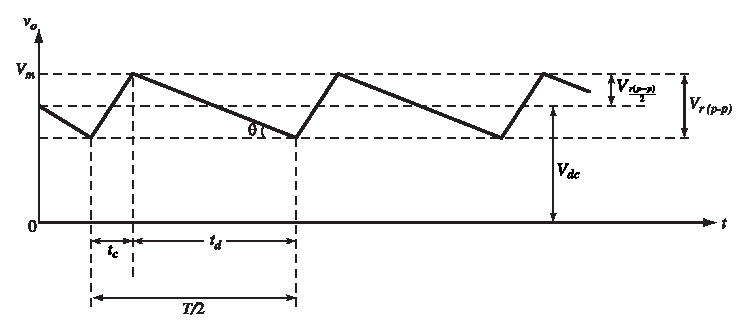
\includegraphics{chap2/add-fig/S3-EE-02-019.eps}
\caption{Ripple voltage on capacitor approximated by triangular waveform}\label{fig2.19}
\end{figure}

From Fig.~\ref{fig2.19},
\begin{align*}
\frac{dv_0}{dt} & = \text{slope of ripple voltage waveform during
  discharge}\\
& = \tan \theta \\
& = \frac{V_{r\,(p-p)}}{t_d}
\end{align*}

Using this relation in equation \eqref{eq2.59}, we have
\begin{align}
I_{dc} & = C\, \frac{V_{r\,(p-p)}}{t_d} \notag\\
V_{r\,(p-p)} & = \frac{I_{dc}\,t_d}{C} \label{eq2.60}\\
\text{Also, \ } \quad \frac{T}{2} & = t_c + t_d \label{eq2.61}
\end{align}

When $C$ is large, $t_c \ll t_d$.

From equation \eqref{eq2.61}, $t_d \simeq \frac{T}{2}$.
\begin{align*}
\text{But} \quad T & = 1/f\\
\therefore ~~ t_d & = \frac{1}{2f}
\end{align*}

Using this relation in equation \eqref{eq2.60}, we have
\begin{align}
V_{r\,(p-p)} & = \frac{I_{dc}}{2 f C} \label{eq2.62}\\
\text{But } ~ ~~ I_{dc} & = V_{dc} / R_L. \notag
\end{align}

Also, from equation \eqref{eq2.58}
$$
V_{r\,(p-p)} = 2 \sqrt{3} V_{ac}.
$$

Using these relations in equation \eqref{eq2.62}, we get
\begin{align}
2 \sqrt{3} V_{ac} & = \frac{V_{dc}}{2 f C R_L}\notag\\[4pt]
\text{Now} ~~~ \gamma &= \frac{V_{ac}}{V_{dc}} = \frac{1}{4 \sqrt{3} f
  R_L\, C}\label{eq2.63}
\end{align}

Comparing equations \eqref{eq2.52} and \eqref{eq2.63}, we find that
the ripple factor of full-wave rectifier with capacitor filter is 50\%
of that in half-wave rectifier with capacitor filter.

\medskip
\noindent{\textbf{{\boldmath$dc$} output voltage,
    {\boldmath$V_{dc}$}}}

The triangular waveform of peak-peak value $V_{r\,(p-p)}$ has an average
value $\dfrac{V_{r\,(p-p)}}{2}$. Therefore, the $dc$ output voltage
$$
V_{dc} = V_m - \frac{V_{r\,(p-p)}}{2}
$$

Substituting for $V_{r\,(p-p)}$ from equation \eqref{eq2.60}, we have
\begin{align}
V_{dc} & = V_m - \frac{1}{2} \left[\frac{I_{dc}}{2 f C} \right]
\notag\\[4pt]
V_{dc} & = V_m - \left[\frac{1}{4 f C} \right] I_{dc} \label{eq2.64}
\end{align}

When the filter capacitor is large, $\dfrac{1}{4 f C} \to 0$

From equation \eqref{eq2.64}, we get
\begin{equation}
V_{dc} \simeq V_m   \label{eq2.65}
\end{equation}

\medskip
\noindent{\textbf{Note:}}
The equation of $\gamma$ and $V_{dc}$ given in equations
\eqref{eq2.63} and \eqref{eq2.64} are also applicable for full-wave
bridge rectifier with capacitor filter. 

\eject

\section{Expression for diode current for a full-wave rectifier
  circuit with capacitor filter}\label{eq2.24}
\index{Full-wave rectifier!diode current}
\begin{figure}[H]
\centering
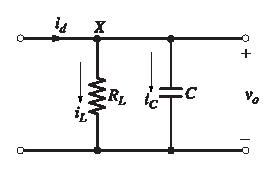
\includegraphics[scale=1.1]{chap2/add-fig/S3-EE-02-020.eps}
\caption{Output circuit of full-wave rectifier with `C' filter}\label{fig2.20}
\end{figure}

The output circuit of a full-wave rectifier with capacitor filter is
shown in Fig. 2.20. From the figure, we see that
\begin{quote}
$i_d$ = Diode current

$i_L$ = Load current

$i_C$ = Capacitor current

$v_0$ = Output voltage
\end{quote}

Using Kirchhoff's Current Law at node $X$, we have
\begin{equation}
i_d = i_L + i_C \label{eq2.66}
\end{equation}

When the diode conducts,
\begin{align}
v_0 & = V_m \sin \omega t \label{eq2.67}\\
i_L & = \frac{v_0}{R_L} = \frac{V_m}{R_L} \sin \omega t \notag\\
i_C & = C\, \frac{dv_0}{dt} = C\, \frac{d}{dt} [V_m \sin \omega t]  = V_m\,
\omega\, C\, \cos \omega t.
\end{align}

Substituting these results in equation \eqref{eq2.66}, we have
\begin{align}
i_d & = \frac{V_m}{R_L} \sin \omega t + V_m\, \omega\, C \cos \omega t\\
& = V_m \left[\frac{1}{R_L} \sin \omega t + \omega\, C \cos \omega t \right] \label{eq2.68}
\end{align}

Multiply and divide the RHS of equation \eqref{eq2.68} by
$\sqrt{(1/R_L)^2 + (\omega C)^2}$
\begin{align}
i_d & = V_m \sqrt{(1/R_L)^2 + (\omega C)^2}\notag\\
& \quad \times \left[\frac{1/R_L}{\sqrt{(1/R_L)^2 + (\omega C)^2}}
  \sin \omega t + \frac{\omega C}{\sqrt{(1/R_L)^2 +(\omega C)^2}} \cos
  \omega t\right] \label{eq2.69}
\end{align}

Assuming a right angle triangle with sides such that 
\begin{center}
\begin{minipage}[c]{9cm}
\begin{align*}
\cos \phi & = \frac{1/R_L}{\sqrt{(1/R_L)^2 + (\omega
    C)^2}}, \\
\text{then } \quad \sin \phi & = \frac{\omega C}{ \sqrt{(1/R_L)^2 +
    (\omega C)^2}}\\
\text{and } \quad \tan \phi & = \omega C R_L \\
 \text{and } \quad I_m  & = V_m \sqrt{(1/R_L)^2 + (\omega C)^2}
\end{align*}
\end{minipage}
\quad
\begin{minipage}[c]{4cm}
\begin{figure}[H]
\centering
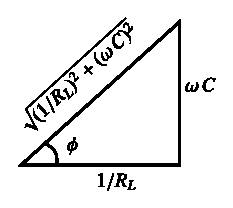
\includegraphics{chap2/eqfig1.eps}
\end{figure}
\end{minipage}
\end{center}

Using these relations in equation \eqref{eq2.69}, we have
\begin{align}
i_d & = I_m [\sin \omega t \cos \phi + \cos \omega t \sin \phi] \notag\\
i_d & = I_m \sin [\omega t + \phi] \label{eq2.70}
\end{align}

Comparing equations \eqref{eq2.67} and \eqref{eq2.70} we find that the
diode current leads the supply voltage by an angle $\phi$. The diode
current given in equation \eqref{eq2.70} is also applicable for bridge
rectifier and half-wave rectifier with capacitor filter. The Summary
of results obtained for half-wave and full-wave rectifiers with
capacitor filter is given in Table~\ref{tab2.5}.
\begin{table}[H]
\centering
\renewcommand{\arraystretch}{1.6}
\tabcolsep=6pt
\caption{Summary of results for half-wave and full-wave
rectifiers with `$C$' filter}\label{tab2.5}
\begin{tabular}{|c|c|c|c|}
\hline
\multirow{2}{1.5cm}{Parameter\index{Rectifier!parameter}} & \multirow{2}{2cm}{Half-wave
  rectifier} &  \multicolumn{2}{c|}{Full-wave rectifier}\\\cline{3-4}
 & & Two diode circuit & Bridge rectifier\\
\hline
Ripple Factor, $\gamma$ & $\dfrac{1}{2\sqrt{3} f R_L C}$ &
$\dfrac{1}{4 \sqrt{3} f R_L(C)}$ & $\dfrac{1}{4 \sqrt{3} f R_L C}$\\[8pt]
\hline
$dc$ output voltage, $V_{dc}$ & $V_m - I_{dc} [1/2 f C]$ & $V_m -
I_{dc} [1/4 f C]$ & $V_m -I_{dc} [1/4 f C]$\\[2pt]
\hline
Diode current, $i_d$ & \multicolumn{3}{c|}{$i_d = I_m \sin [\omega t +
  \phi]$}\\[2pt]
&  \multicolumn{3}{c|}{$I_m = V_m \sqrt{(1/R_L)^2 + (\omega C)^2}, ~~
  \phi = \tan^{-1} [\omega C R_L]$}\\
\hline
\end{tabular}
\end{table}

\begin{example}\label{exam2.16}
In a Full Wave Rectifier (FWR) with capacitor filter, the load current
from the circuit operating from 230 V, 50 Hz supply is 10 mA. Estimate
the value of capacitor required to keep the ripple factor less than 1\,\%. 
\end{example}

\begin{solution}
Given,
\begin{align*}
V_2 & = 230 \V.\\[3pt]
V_m & = \sqrt{2}\, V_2 = \sqrt{2}\times 230\V=325.27\V\\[3pt]
f & = 50 \Hz\\[3pt]
I_{dc} & = 10 \mA.\\[3pt]
\% ~ \gamma & < 1 ~~ \Rightarrow ~~ \gamma < 0.01 \\[3pt]
\gamma & =\frac{1}{4 \sqrt{3} f R_L C} < 0.01
\end{align*}

Taking reciprocal on both sides
\begin{align*}
4 \sqrt{3} f R_L C & > 100 \\[3pt]
C& > \frac{100}{4 \sqrt{3} f R_L} \tag{A}\label{eqA}\\[3pt]
R_L & = \frac{V_{dc}}{I_{dc}}
\end{align*}

Taking $V_{dc} \simeq  V_m$  [Refer equation \eqref{eq2.65}]
\begin{align*}
R_L & = \frac{V_m}{I_{dc}}\\[3pt]
& = \frac{325.27 \V}{10 \mA}\\[3pt]
& = 32.53 ~\text{K\,}\Omega
\end{align*}

Now, from equation \eqref{eqA}
\begin{align*}
C & > \frac{100}{4 \sqrt{3} (50) (32.53 \times 10^3)}\\[3pt]
C & > 8.87 \mu F
\end{align*}
\vskip -.9cm
\end{solution}

\eject

\begin{example}\label{exam2.17}
In a FWR with a capacitor filter, the load current from the circuit
operating from 200 V, 50 Hz supply is 12 mA. Calculate the minimum
value of capacitance used in the filter required to keep the ripple
voltage below 2\,\%.
\end{example}

\begin{solution}
Given,
\begin{align*}
V_2 & = 200 \V \\[3pt]
V_m & = \sqrt{2}\, V_2 = 282.84 \V \\[3pt]
f & = 50 \Hz\\[3pt]
I_{dc} & = 12 \mA\\[3pt]
\% ~ \gamma & < 2 \\[3pt]
\text{or } \quad \gamma &< 0.02\\[3pt]
\gamma & = \frac{1}{4 \sqrt{3} ~f R_L C} < 0.02
\end{align*}

Taking reciprocal on both sides
\begin{align*}
4 \sqrt{3} f R_L  C & > 50 \\[3pt]
C & > \frac{50}{4 \sqrt{3} f R_L} \tag{A}\label{eqA}\\[3pt]
R_L & = \frac{V_{dc}}{I_{dc}} \simeq \frac{V_m}{I_{dc}}\\[3pt]
R_L & = \frac{282.84 \V}{12 \mA}\\[3pt]
&= 23.57 ~k  \Omega
\end{align*}

Now, from equation \eqref{eqA},
\begin{align*}
C & > \frac{50}{4 \sqrt{3} (50) (23.57 \times 10^3)}\\[3pt]
C & > 6.12 ~ \mu \F\\[3pt]
C_{\min} & = 6.12 ~ \mu \F
\end{align*}
\vskip -.9cm
\end{solution}

\eject

\begin{example}\label{2.18}
A full-wave rectifier using two diodes supplies a load of 2
k$\Omega$. The $ac$ voltage applied to the diodes is 200\,V-0-200\,V. If a
capacitor of value 500 $\mu$F is connected across the load, find (a)
Ripple factor (b) $dc$ output voltage (c) Ripple voltage on capacitor
(d) DC load current.
\end{example}

\begin{solution}
Given,
\begin{align*}
V_2 & = 200 ~\V.\\[3pt]
V_m & = 200 \sqrt{2} = 282.84 ~ \V.\\[3pt]
f & = 50 ~\Hz\\[3pt]
C & = 500 ~ \mu \F \\[3pt]
R_L & = 2 ~ \kk \Omega
\end{align*}

\begin{itemize}
\item[(a)] Ripple Factor, $\gamma$
\begin{align*}
\gamma & = \frac{1}{4 \sqrt{3} f R_LC}\\
& = \frac{1}{4 \sqrt{3} (50) (2000) (500 \times 10^{-6})}\\[3pt]
& = 2.89 \times 10^{-3} \text{~ or ~} 0.289 ~\%  
\end{align*}

\item[(b)] $dc$ output voltage, $V_{dc}$
\begin{align*}
V_{dc} & = V_m - I_{dc} \left[\frac{1}{4 f C} \right]\\[3pt]
I_{dc} & = \frac{V_{dc}}{R_L}\\[3pt]
V_{dc} & = V_m - V_{dc} \left[\frac{1}{4 f C R_L} \right]\\[3pt]
\text{Solving, ~~} V_{dc} & = \frac{V_m}{1 + \left[\frac{1}{4 f C R_L}
    \right]}\\[3pt]
& = \frac{282.84\text{\,V}}{1 + \left[\frac{1}{4 (50) (500 \times 10^{-6}) (2000)} \right]}\\[3pt]
& = 281.43 ~\V.
\end{align*}

\eject

\item[(c)] Ripple voltage on capacitor, $V_{ac}$
\begin{align*}
\gamma & = \frac{V_{ac}}{V_{dc}} \\[3pt]
V_{ac} & = \gamma  V_{dc}\\[3pt]
& = 2.89 \times 10^{-3}  \times 281.43\text{\,V}\\[3pt]
& = 0.8133 ~ \V.
\end{align*}

\item[(d)] DC load current, $I_{dc}$
\begin{align*}
I_{dc} & = \frac{V_{dc}}{R_L}\\[3pt]
& = \frac{281.43\text{\,V}}{2000\Omega}\\[3pt]
& = 0.1407 ~ \A
\end{align*}
\end{itemize}
\vskip -.9cm
\end{solution}

\begin{example}\label{exam2.19}
A single-phase full-wave rectifier supplies a load of 250
$\Omega$. The transformer secondary voltage with reference to centre
tap is $35 \V (rms)$ at 50 Hz. Find the ripple factor and $dc$ output
voltage if a capacitor of 160 $\mu$F is connected in parallel with the
load. 
\end{example}

\begin{solution}
Given,
\begin{align*}
R_L & = 250 ~ \Omega\\[3pt]
C & = 160 ~ \mu \F \\[3pt]
f & = 50 \Hz\\[3pt]
V_2 & = 35 \V \\[3pt]
 V_m & = \sqrt{2}\, V_2 = 49.497 ~\V
\end{align*}

\begin{itemize}
\item[(a)] Ripple factor, $\gamma$
\begin{align*}
\gamma & = \frac{1}{4 \sqrt{3}f R_L C}\\
& = \frac{1}{4 \sqrt{3} (50) (250) (160 \times 10^{-6})}\\
 &= 0.0722 \text{~ or ~} 7.22 \%
\end{align*}

\eject

\item[(b)] $dc$ output voltage, $V_{dc}$
\begin{align*}
V_{dc} & = \frac{V_m}{1 + \left[\frac{1}{4 f C R_L} \right]}\\[3pt]
& = \frac{49.5\text{\,V}}{1+ \left[\frac{1}{4 \times 50 \times 160 \times
      10^{-6} \times 250} \right]}\\[3pt]
& = 44 ~ \V
\end{align*}
\end{itemize}
\vskip -.9cm
\end{solution}

\begin{example}\label{exam2.20}
A full-wave bridge rectifier supplies a load of 400 $\Omega$ in parallel
with a capacitor of 500 $\mu$F. If the $ac$ supply voltage is 230 sin\,
314\,t V, find the 
\begin{itemize}
\item[(a)] Ripple factor and

\item[(b)] DC load current
\end{itemize}
\end{example}

\begin{solution}
Given, 
\begin{align*}
V_m \sin \omega t & = 230 \sin 314~ t \\[2pt]
\Rightarrow\qquad V_m & = 230 \V\\[2pt]
\omega & = 2 \pi f = 314~ r/s\\[2pt]
f & = \frac{314}{2\pi} = 50 \Hz\\[2pt]
R_L & = 400\,\Omega\\[2pt]
C & = 500 ~\mu F
\end{align*}
\begin{itemize}
\item[(a)] Ripple factor, $\gamma$
\begin{align*}
\gamma & = \frac{1}{4 \sqrt{3} f R_L C}\\
& = \frac{1}{4 \sqrt{3} (50) (400) (500 \times 10^{-6})}\\[2pt]
& = 0.0144 \text{ ~ or ~} 1.44\%
\end{align*}

\item[(b)] DC load current, $I_{dc}$
\begin{align*}
V_{dc} & = \frac{V_m}{1 + \left[\frac{1}{4 f C R_L} \right]}\\
& = \frac{230\text{\,V}}{1+ \left[ \frac{1}{4 \times 50 \times 500 \times
      10^{-6} \times 400}\right]}\\[3pt]
& = 224.39 ~\V\\[3pt]
I_{dc} & = \frac{V_{dc}}{R_L}\\[3pt]
& = \frac{224.39\text{\,V}}{400\,\Omega}\\[3pt]
& = 0.56 ~ \A
\end{align*}
\end{itemize}
\vskip -1cm
\end{solution}

\begin{example}\label{exam2.21}
A half-wave rectifier $dc$ power supply has to supply 20 V to a 500
$\Omega$ load. The peak-peak ripple voltage should not exceed 10\,\%
of the average output voltage and the $ac$ input frequency is 60
Hz. Calculate the required capacitor value.
\end{example}

\begin{solution}
Given,
\begin{align*}
V_2 & = 20 ~ \V \\[3pt]
V_m & = \sqrt{2}\times 20\V = 28.28 ~ \V \\[3pt]
f & = 60 ~ \Hz\\[3pt]
R_L & = 500 ~ \Omega\\[3pt]
V_{r\,(p-p)} & = 10 \% \text{~ of ~} ~V_{dc} \\[3pt]
\text{i.e., } ~~ V_{r\,(p-p)} & = 0.1 ~V_{dc}\\[3pt]
\text{But } ~~ V_{r\,(p-p)} & = 2 \sqrt{3}\, V_{ac} \\[3pt]
\therefore ~~ 2 \sqrt{3}\, V_{ac} & = 0.1 V_{dc}\\[3pt]
\gamma & = \frac{V_{ac}}{V_{dc}} = \frac{0.1}{2\,\sqrt{3}} = 0.02886\\[3pt]
\gamma & = \frac{1}{2 \sqrt{3} f R_L C}\\[3pt]
C& = \frac{1}{2 \sqrt{3}\, \gamma\, f\, R_L}\\[3pt]
 & = \frac{1}{2 \sqrt{3} (0.028) (60) (500)}\\[3pt]
C & = 343.66  ~ \mu \F
\end{align*}
\vskip -1cm
\end{solution}

\begin{example}\label{exam2.22}
A full-wave rectifier $dc$ power supply has to supply 20 V to a 500
$\Omega$ load. The peak-peak ripple voltage is not to exceed 10\% of the
average output voltage and the $ac$ input frequency is 60
Hz. Calculate the required filter capacitor value.
\end{example}

\begin{solution}
Given, 
\begin{align*}
V_2 & = 20 \V \\[3pt]
V_m & = \sqrt{2} ~ V_2 = 28.28 \V\\[3pt]
f & = 60 \Hz\\[3pt]
R_L & = 500 ~\Omega\\[3pt]
V_{r\,(p-p)} & = 0.1 ~V_{dc}\\[3pt]
2 \sqrt{3}\, V_{ac} & = 0.1 V_{dc} \\[3pt]
\frac{V_{ac}}{V_{dc}} & = \gamma = \frac{0.1}{2 \sqrt{3}} = 0.02886\\[3pt]
\gamma & = \frac{1}{4 \sqrt{3} f R_L C}\\[3pt]
C & = \frac{1}{4 \sqrt{3} f R_L\, \gamma} = \frac{1}{4 \sqrt{3} (60)
  (500) (0.028)}\\[3pt]
&  = 171.83 ~ \mu \F
\end{align*}
\vskip -1cm
\end{solution}

\section{\boldmath$dc$ Power Supply}\label{sec2.25}
\index{dc@$dc$ Power Supply}

A $dc$ power supply consists of a rectifier which converts an $ac$ to $dc$ and a filter which reduces the ripple content of the rectified output to a tolerable level. A $dc$ power supply is required to provide a constant $dc$ voltage over a range of load current varying from zero to a specified maximum value $I_{L(\max)}$.

The $dc$ output voltage of a full-wave rectifier with capacitor filter is given by
\begin{equation}
V_{dc}=V_{m}-I_{dc}[1/4\, f \ C]\label{eq2.73}
\end{equation}
\begin{quote}
$V_{dc}$ is also denoted by $V_{o}$.

$V_{m}$ is the peak transformer secondary voltage and

$I_{dc}$ is the DC load current which is also denoted by $I_{L}$.
\end{quote}

From the above equation we find that the $dc$ output voltage $V_{dc}$ is a function of the $ac$ supply voltage $V_{m}$ and the load current $I_{L}$. The $ac$ supply voltage is also called as the line voltage.

The variation in $dc$ output voltage due to variation in line voltage is called source effect and the variation in $dc$ output voltage with load current is called load effect.

The source effect and load effect are the performace measures of a $dc$ power supply.

\section{Line Regulation and Load Regulation as Applied to $dc$ Power Supplies}\label{sec2.26}

The $dc$ output voltage in a $dc$ power supply varies due to
\begin{itemize}
\item[(a)] the source effect\index{dc@$dc$ Power Supply!source effect} and

\item[(b)] the load effect.\index{Load effect}
\end{itemize}

\heading{Source effect~:}\index{Source effect}
The $ac$ supply to the input of a transformer of a $dc$ power supply does not remain constant. $A\pm 10\%$ variation in the $ac$ supply voltage $V_{s}$ also called as the line voltage is very common. There is some variation in the $dc$ output voltage when the line voltage varies. The output voltage change $\Delta V_{o}$ due to a change in the line voltage is called the source effect.
\begin{equation}
\text{Source effect = } \Delta V_{o}\text{~~ for a~~ } 10\%\text{~~ change in~~ } V_{s}\label{eq2.74}  
\end{equation}

For example, if the output varies by 100\,mV when the source voltage changes by $\pm 10\%$, the source effect is 100\,mV. The source effect expressed as a percent of $dc$ output voltage $V_{o}$, is called the line regulation
\begin{equation}
\therefore\quad \text{Line regulation = } \dfrac{\Delta V_{o}\text{~~ for a~~ } 10\%\text{~~ change in~~ }V_{s}}{V_{o}}\times 100\,\%\label{eq2.75}
\end{equation}

For a good $dc$ power supply $\Delta V_{o}$ should be very small. Ideally, $\Delta V_{o}=0$. Therefore, line regulation is zero percent for an ideal $dc$ power supply.

\medskip
\heading{Load effect~:}\index{dc@$dc$ Power Supply!load effect}
The $dc$ output voltage $V_{o}$ is a function of the load current $I_{L}$ (see Eqn.~\eqref{eq2.73}). If the load current $I_{L}$ increases, $V_{o}$ decreases and $V_{o}$ increases when the load current is reduced. The load effect defines how the output voltage changes when the load current is increased from zero to its specified maximum value $I_{L(\max)}$. The output voltage change $\Delta V_{o}$ due to the load current change $\Delta I_{L(\max)}$ is called load effect.

Fig.~\ref{fig2.21} depicts the source effect in a $dc$ power supply.
\begin{equation}
\text{Load effect = } \Delta V_{o}\text{~~ for~~ } \Delta I_{L(\max)}\label{eq2.76}
\end{equation}

For example, if the load current change $\Delta I_{L}$ produces a voltage change $\Delta V_{o}$ of 100\,mV, the load effect is 100\,mV. The load effect expressed as a percentage of the output voltage $V_{o}$, is called the load regulation.
\begin{equation}
\text{Load regulation = } \dfrac{\Delta V_{o}\text{~~ for~~ } \Delta I_{L(\max)}}{V_{o}}\times 100\label{eq2.77}
\end{equation}
For a good power supply, $\Delta V_{o}$ should be very small, ideally, $\Delta V_{o}=0$. Therefore, load regulation is zero for an ideal $dc$ power supply.
\setcounter{figure}{20}
\begin{figure}[H]
\centering
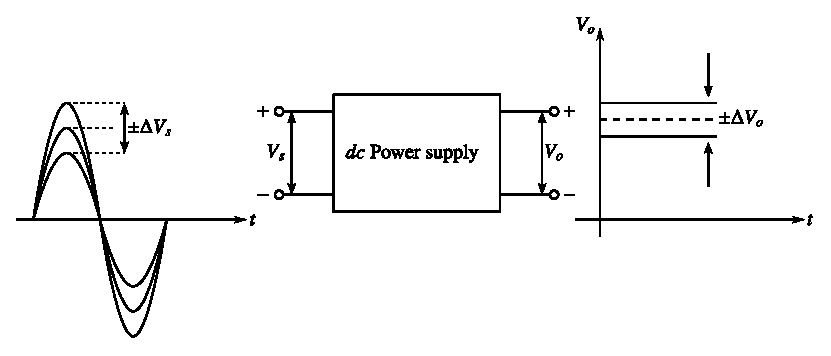
\includegraphics{chap2/fig2.21.eps}
\caption{Source effect in a $dc$ power supply}\label{fig2.21}
\end{figure}

\begin{example}\label{exam2.23}
The output voltage of a $dc$ power supply changes from 20\,V to 19.7\,V when the load is increased from zero to maximum. The voltage also increases to 20.2\,V when the $ac$ supply increases by 10\,\%. Calculate the load and source effect and the load and line regulations.
\end{example}

\begin{solution}
Given,
\begin{align*}
\text{load effect~} &= \Delta V_{o}\text{~~ for~~ }\Delta I_{L}(\max)\\[3pt]
&= 20V-19.7V\\[3pt]
&= 300\text{\,mV}\\[3pt]
\text{Load regulation~} &= \dfrac{\Delta V_{o}\text{~~ for~~ }\Delta I_{L}(\max)}{V_{o}}\times 100\,\%\\[3pt]
&= \frac{300\text{\,mV}\times 100}{20V}\,\%\\[3pt]
&= 1.5\%\\[3pt]
\text{Source effect} &= \Delta V_{o}\text{~~ for~~ } 10\,\%\text{~~ change in~~ } V_{s}\\[3pt]
&= 20.2\text{\,V}-20\\[3pt]
&= 200\text{\,mV}\\[3pt]
\text{Line regulation~} &= \frac{\Delta V_{o}\text{~~ for~~ } 10\,\%\text{~~ change in~~ }V_{s}}{V_{o}}\times 100\,\%\\[3pt]
&=\frac{200\text{\,mV}\times 100}{20\text{\,V}}\\[3pt]
&= 1\,\%
\end{align*}
\vskip -1cm
\end{solution}

\begin{example}\label{exam2.24}
A $dc$ power supply output drops from 15\,V to 14.95\,V when the $ac$ source voltage falls by 10\,\%. The output also falls from 15\,V to 14.9\,V when the load current is increased from zero to maximum. Calculate the source effect, load effect, line regulation and load regulation.
\end{example}

\begin{solution}
Given,
\begin{align*}
\text{Load effect } &= \Delta V_{o}\text{~~ for~~ }\Delta I_{L}(\max)
= 15\text{\,V}-14.9\text{\,V}\\[3pt]
&= 0.1\text{\,V}\\[3pt]
\text{Load regulation } &= \dfrac{\Delta V_{o}\text{~~ for~~ }\Delta I_{L}(\max)}{V_{o}}\times 100\,\%\\[3pt]
&= \frac{0.1\text{\,V}}{15\,\text{V}}\times 100
= 0.66\,\%\\[3pt]
\text{Source effect } &= \Delta V_{o}\text{~~ for~~ } 10\,\%\text{~~ change in~~ } V_{s}\\[3pt]
&= 15\text{\,V}-14.95\text{\,V}= 0.05\text{\,V}\\[3pt]
\text{Line regulation } &= \frac{\Delta V_{o}\text{~~ for~~ }10\,\%\text{~~ change in~~ } V_{s}}{V_{o}}\times 100\\[3pt]
&= \frac{0.05\text{\,V}}{15\text{\,V}}\times 100= 0.33\,\%
\end{align*}
\vskip -1cm
\end{solution}

\section{Voltage Regulator}\label{sec2.27}
\index{Voltage Regulator}

A voltage regulator is a circuit which accepts unregulated $dc$ as input and provides a constant $dc$ output voltage irrespective of changes in the line voltage and the load current.

The output of a full-wave rectifier with capacitor filter may be called unregulated $dc$ since it varies with changes in load current and line voltage. Most of the electronic circuits require a stable $dc$ voltage for their proper operation. Hence, it is necessary to regulate the output of full-wave rectifier with filter. A voltage regulator is connected between the full-wave rectifier with filter and the load as shown in Fig.~\ref{fig2.22}.
\begin{figure}[H]
\centering
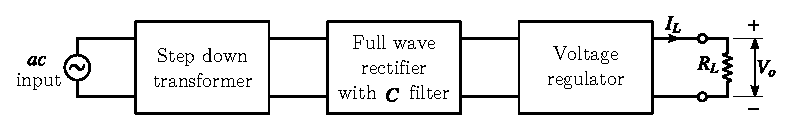
\includegraphics{chap2/fig2.22.eps}
\caption{Block diagram of regulated $dc$ power supply}\label{fig2.22}
\end{figure}

\section{Zener Diode Voltage Regulator}\label{sec2.28}

An important application of Zener diode\index{Zener diode} is in $dc$ voltage regulator circuit. The reason is that, under reverse breakdown condition, the voltage across Zener remains constant over a wide range of reverse current, $I_{ZK}<I_{Z}<I_{ZM}$ \ as \ shown in Fig.~\ref{fig1.28}.

$I_{ZK}$ is the minimum reverse current to sustain breakdown.

$I_{ZM}$ is the maximum Zener current, limited by the maximum power dissipation $(P_{D})$.
$$
P_{D}=V_{Z}\,I_{ZM}
$$

\subsection{Zener diode voltage regulator under no load}\label{sec2.28.1}
\index{Zener diode!voltage regulator}

Fig.~\ref{fig2.23} shows the Zener diode used as voltage regulator under no load (i.e., $I_{L}=0$).
\begin{figure}[H]
\centering
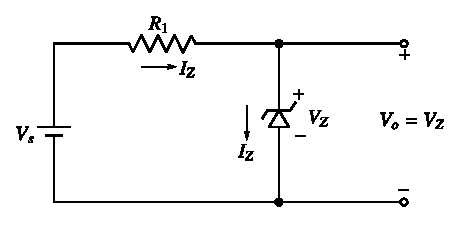
\includegraphics{chap2/fig2.23.eps}
\caption{Zener diode voltage regulator under no load}\label{fig2.23}
\end{figure}

$V_{s}$ is the unregulated $dc$ voltage, which may be the output from a full-wave rectifier with capacitor filter. 

Since the Zener diode is connected across the output terminals,
\begin{equation}
V_{0}=V_{Z}=\text{~ constant}\label{eq2.78}
\end{equation}

Also, since $V_{s}$ is an unregulated DC voltage, it is likely to change. The change in $V_{s}$ is absorbed across $R_{1}$ since $V_{0}$ is a constant.

For the circuit to work properly.
\begin{itemize}
\item The unregulated $dc$ voltage, $V_{s}$, must be greater than the Zener breakdown voltage, $V_{Z}$.

\item The current $I_{Z}$ must satisfy the condition
$$
I_{ZK}<I_{Z}<I_{ZM}
$$

\item $I_{Z}>I_{ZK}$, ensures the minimum reverse current to sustain breakdown.

\item $I_{Z}<I_{ZM}$, ensures the safe operation of Zener diode by keeping the power dissipation less than the maximum permissible value $(P_{D})$.
\end{itemize}

Applying KVL to the circuit of Fig.~\ref{fig2.23}, we have
\begin{align}
& V_{s}-I_{Z}\,R_{1}-V_{Z}=0\label{eq2.79}\\[3pt]
& I_{Z}=\frac{V_{s}-V_{Z}}{R_{1}}\label{eq2.80}
\end{align}

Normally $I_{Z}$ is selected as $I_{ZT}$ (the specified test current) in order to obtain the most stable reference voltage. It is important to note that, $I_{ZT}$ lies between $I_{ZK}$ and $I_{ZM}$ as shown in the Zener diode characteristics of Fig.~\ref{fig1.28}.

\begin{example}\label{exam2.25}
A 12\,V reference source is to use a series - connected Zener diode and resistor connected to a 30\,V supply. Select suitable components and calculate the circuit current when the supply voltage drops to 25\,V.
\end{example}

\begin{solution}
Given,
\begin{align*}
V_{s} &= 30\text{\,V}\\[3pt]
V_{o} &= 12\text{\,V}\Rightarrow V_{Z}=12\text{\,V}
\end{align*}

Select a Zener diode with
$$
V_{Z}=12\text{\,V}\quad\text{and}\quad I_{ZT}=20\text{\,mA}\qquad\text{(Typical value)}
$$
\begin{align*}
R_{1} &= \frac{V_{s}-V_{Z}}{I_{Z}}\tag{A}\\[3pt]
I_{Z} &= I_{ZT}=20\text{\,mA}\\[3pt]
\therefore\quad R_{1} &= \frac{30\text{\,V}-12\text{\,V}}{20\text{\,mA}}=900\,\Omega
\end{align*}
Power dissipation is $R_{1}$~:
\begin{align*}
P_{R_{1}} &= (I_{ZT})^{2}R_{1}=(200\text{\,mA})^{2}(900\,\Omega)\\[3pt]
&= 0.36W
\end{align*}

\eject

The required circuit is shown below.
\begin{figure}[H]
\centering
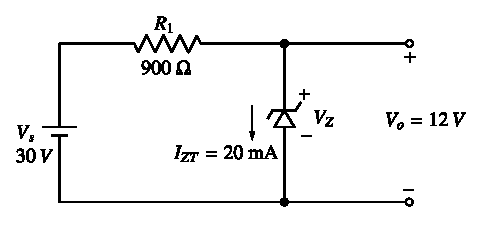
\includegraphics{chap2/sol2.26.eps}
\end{figure}

\noindent
when $V_{s}=25\text{\,V}$~:

From Eqn.~(A)
\begin{align*}
I_{Z} &= \frac{V_{s}-V_{Z}}{R_{1}}=\dfrac{25\text{\,V}-12\text{\,V}}{900\,\Omega}\\[3pt]
&= 14.44\text{\,mA}
\end{align*}
\end{solution}

\begin{example}\label{exam2.26}
Design a 9\,V $dc$ reference source consisting of a Zener diode and series connected resistor to operate from a 24\,V supply. Determine the effect on the diode current when the supply voltage drops to 20\,V.
\end{example}

\begin{solution}
Given,
\begin{gather*}
V_{s}=24\text{\,V}\\[3pt]
V_{o}=9\text{\,V}\Rightarrow V_{Z}=9\text{\,V}
\end{gather*}

Select a Zener diode with $V_{Z}=9V$ and $I_{ZT}=20\mA$ (Typical)
\begin{align*}
R_{1} &= \frac{V_{s}-V_{Z}}{I_{Z}}=\frac{V_{s}-V_{Z}}{I_{ZT}}\\[3pt]
&=\frac{24\text{\,V}-9\text{\,V}}{20\text{\,mA}}\\[3pt]
&= 750\,\Omega
\end{align*}
Power dissipation in $R_{1}$~:
\begin{align*}
P_{R_{1}} &= (I_{Z_{T}})^{2}R_{1}=(20\text{\,mA})^{2}(750\,\Omega)\\[3pt]
&= 0.3W
\end{align*}

\eject

The required circuit is shown below
\begin{figure}[H]
\centering
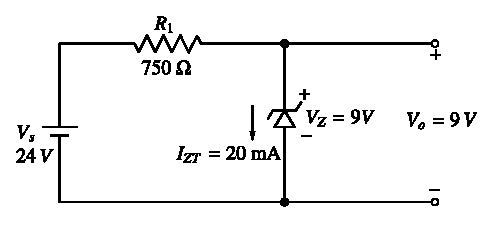
\includegraphics{chap2/sol2.27.eps}
\end{figure}
when the supply voltage drops to $20\V$.
$$
I_{Z}=\dfrac{V_{S}-V_{Z}}{R_{1}}=\dfrac{20\V-9\V}{750\Omega}=14.66\text{\,mA}
$$
\vskip -1cm
\end{solution}

\begin{example}\label{exam2.28}
A Zener diode has a breakdown voltage of 10\,V. It is supplied from a voltage source varying between 20 and 40\,V in series with a resistance of 820\,$\Omega$. Using an ideal Zener diode model obtain minimum and maximum Zener currents. 
\end{example}

\begin{solution}
\begin{align*}
& V_{Z}=10\text{\,V}\quad R_{1}=820\Omega\\[3pt]
& V_{s}:20\text{\,V}-40\text{\,V}\\[3pt]
\Rightarrow\quad & V_{s\min} = 20\text{\,V}\quad V_{s\max}=40\text{\,V}\\[3pt]
& I_{Z}=\frac{V_{s}-V_{Z}}{R_{1}}\tag{A}
\end{align*}
when\, $V_{s}=V_{s\min}$,\, $I_{Z}=I_{Z\min}$.

\vskip .1cm

From Eqn.~(A)
\begin{align*}
I_{Z\min} &= \frac{V_{s\min}-V_{Z}}{R_{1}}=\frac{20\,\text{V}-10\text{V}}{820\,\Omega}\\[3pt]
&= 12.19\text{\,mA}
\end{align*}
when\, $V_{s}=V_{s\max}$,\, $I_{Z}=I_{Z\max}$.

\vskip .1cm

Again from Eqn.~(A)
\begin{align*}
I_{Z\max} &= \frac{V_{s\max}-V_{Z}}{R_{1}}=\frac{40\text{\,V}-10\text{\,V}}{820\,\Omega}\\[3pt]
&= 36.58\text{\,mA}
\end{align*}
\vskip -1cm
\end{solution}

\eject

\subsection{Loaded Zener diode voltage regulator}\label{sec2.28.2}

Fig.~\ref{fig2.24} shows the circuit of Zener diode voltage\index{Rectifier!voltage ragulator} regulator supplying the load current $I_{L}$, to the load $R_{L}$.
\begin{figure}[H]
\centering
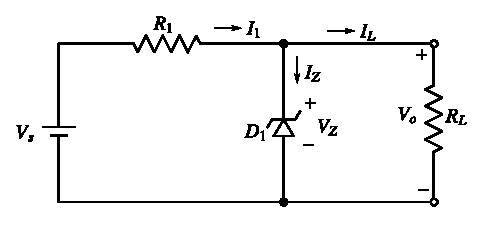
\includegraphics{chap2/fig2.24.eps}
\caption{Zener diode voltage regulator supplying a load current}\label{fig2.24}
\end{figure}
Current through $R_{1}$ is the sum of $I_{L}$ and $I_{Z}$
\begin{equation}
\therefore\quad I_{1}=I_{Z}+I_{L}\label{eq2.81}
\end{equation}

Applying KVL to the path containing $V_{s}-R_{1}-V_{Z}$, we have,
\begin{equation}
V_{s}-I_{1}R_{1}-V_{Z}=0\label{eq2.82}
\end{equation}

Voltage across $R_{1}$ is
\begin{align*}
& I_{1}R_{1}=V_{s}-V_{Z}=\text{~constant}\\[3pt]
\Rightarrow\qquad & I_{1}\text{~~ is a constant}
\end{align*}

Also from Eqn.~\eqref{eq2.82}, we get
\begin{equation}
I_{1}=\frac{V_{s}-V_{Z}}{R_{1}}\label{eq2.83}
\end{equation}

In a practical voltage regulator, the load current varies between zero (no load) and a maximum, $I_{L\max}$.

When the load current is maximum i.e., $I_{L}=I_{L\max}$, from Eqn.~\eqref{eq2.81} we find that, $I_{Z}$ is a minimum i.e., $I_{Z}=I_{Z\min}$. Care must be taken to ensure that, $I_{Z\min}$ is large enough to keep the diode in reverse breakdown. From Eqn.~\eqref{eq2.81}, with $I_{L}=I_{L\max}$, we get,
\begin{equation}
I_{1}=I_{Z\min}+I_{L\max}\label{eq2.84}
\end{equation}

For a Zener diode with an $I_{ZT}$ of $20\,\text{mA}$, the typical value of $I_{Z\min}$ is $5\text{\,mA}$.

When the load current is zero, the entire $I_{1}$ flows through the Zener diode. The circuit design must ensure that the total current does not exceed the maximum Zener diode current, $I_{ZM}$.

From Eqn.~\eqref{eq2.81} with $I_{L}=0$, we get
\begin{equation}
I_{1}=I_{ZM}\label{eq2.85}
\end{equation}

Combining Eqns.~\eqref{eq2.84} and \eqref{eq2.85} we get
\begin{equation}
I_{ZM}=I_{Z\min}+I_{L\max}\label{eq2.86}
\end{equation}

Using Eqn.~\eqref{eq2.85}, we can also write Eqn.~\eqref{eq2.83} as
\begin{equation}
R_{1}=\frac{V_{S}-V_{Z}}{I_{ZM}}\label{eq2.87}
\end{equation}

From Eqn.~\eqref{eq2.86} we note that,
$$
I_{ZM}>I_{L\max}
$$

\begin{example}\label{exam2.28}
Design a 6\,V $dc$ reference source to operate from a 15\,V supply. The circuit has to provide a maximum possible load current. Calculate the maximum load current that can be drawn from the circuit. Use a suitable low power Zener diode.
\end{example}

\begin{solution}
Given,
\begin{gather*}
V_{S}=15\text{\,V}\\[3pt]
V_{o}=6\text{\,V}\Rightarrow V_{Z}=6\text{\,V}
\end{gather*}

Select a low power Zener diode with
$$
V_{Z}=6\text{\,V},\quad I_{ZT}=20\text{\,mA},\quad P_{D}=400\text{\,mW}
$$
we take $I_{Z\min}=5\text{\,mA}$\quad (Typical)
\begin{align*}
I_{ZM} &= \frac{P_{D}}{V_{Z}}=\frac{400\text{\,mW}}{6\text{\,V}}\\[4pt]
&= 66.67\text{\,mA}\\[4pt]
R_{1} &= \frac{V_{S}-V_{Z}}{I_{ZM}}=\frac{15\text{\,V}-6\text{\,V}}{66.67\text{\,mA}}\\[4pt]
&= 135\,\Omega.
\end{align*}

\eject

Power dissipation in $R_{1}$~:
\begin{align*}
P_{R_{1}} &= (I_{ZM})^{2}R_{1}=(66.67\text{\,mA})^{2}(135\,\Omega)\\[3pt]
&= 0.6\text{\,W}\\[3pt]
I_{ZM} &= I_{L\max}+I_{Z\min}\\[3pt]
I_{L\max} &= I_{ZM}-I_{Z\min}=66.67\text{\,mA}-5\text{\,mA}\\[3pt]
&= 61.67\text{\,mA}\\[3pt]
R_{L\min} &= \frac{V_{o}}{I_{L\max}}=\frac{6\text{\,V}}{61.67\text{\,mA}}\\[3pt]
&= 97.3\,\Omega
\end{align*}

The required circuit is shown below.
\begin{figure}[H]
\centering
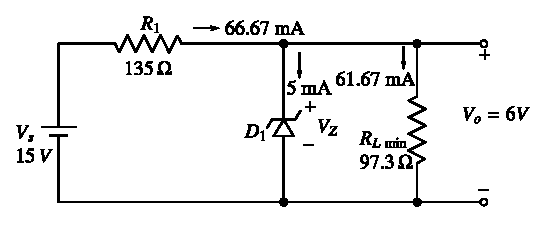
\includegraphics{chap2/sol2.26a.eps}
\end{figure}
\vskip -1cm
\end{solution}

\begin{example}\label{exam2.29}
A series connected Zener diode and a resistor are to be used as a 10\,V reference source with a load current of 15\,mA. The available supply voltage is 25\,V. Select suitable components.
\end{example}

\begin{solution}
Given,
\begin{gather*}
V_{S} = 25\,\text{V}\\[3pt]
V_{o}=10\text{\,V}\Rightarrow V_{Z}=10\text{\,V}
\end{gather*}

Select a low power Zener diode with
$$
V_{Z}=10\text{\,V},\quad I_{ZT}=20\text{\,mA},\quad P_{D}=400\text{\,mW}
$$
Choose $I_{Z\min}=5\text{\,mA}$\quad (Typical)
\begin{align*}
I_{ZM} &= \frac{P_{D}}{V_{Z}}=\frac{400\text{\,mW}}{10}\\[3pt]
&= 40\text{\,mA}\\[3pt]
R_{1} &= \frac{V_{s}-V_{Z}}{I_{ZM}}=\frac{25\text{\,V}-10\text{\,V}}{40\text{\,mA}}\\[3pt]
&= 375\,\Omega
\end{align*}
Power dissipation in $R_{1}$~:
\begin{align*}
P_{R_{1}} &= (I_{ZM})^{2}R_{1}=(40\text{\,mA})^{2}(375\,\Omega)\\[3pt]
&= 0.6\text{\,W}
\end{align*}
Load current, $I_{L}=15\text{\,mA}$
\begin{align*}
\therefore\quad R_{L} &= \frac{V_{o}}{I_{L}}=\frac{10\text{\,V}}{15\text{\,mA}}\\[3pt]
&= 666.67\Omega
\end{align*}
The required circuit is shown below.
\begin{figure}[H]
\centering
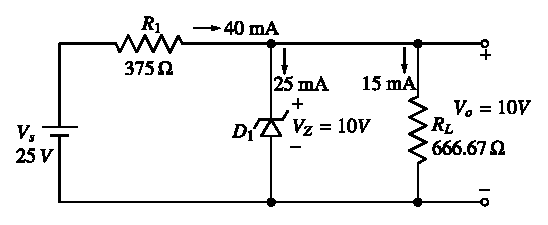
\includegraphics{chap2/sol2.27a.eps}
\end{figure}
\vskip -1cm
\end{solution}

\begin{example}\label{exam2.30}
A 24\,V, 600\,mW, Zener diode is used for providing a 24\,V stabilized supply to a variable load. If the input voltage is 32\,V, calculate the following.
\begin{itemize}
\item[(i)] the value of series resistance required.

\item[(ii)] the diode current when $R_{L}=2.4\,k\Omega$.

\item[(iii)] the minimum value of $R_{L}$ that can be connected across the regulator.
\end{itemize}
\end{example}

\begin{solution}
Given
\begin{align*}
V_{s} &= 32\text{\,V}\\[3pt]
V_{o} &= V_{Z}=24\text{\,V}\qquad P_{D}=600\text{\,mW}\\[3pt]
I_{ZM} &= \frac{P_{D}}{V_{Z}}=\frac{600\,\text{mW}}{24\text{\,V}}\\[3pt]
&= 25\text{\,mA}
\end{align*}
\begin{itemize}
\item[(i)]
\begin{tabbing}
~$R_{1}$ \== $\dfrac{V_{s}-V_{Z}}{I_{ZM}}=\dfrac{32\text{\,V}-24\text{\,V}}{25\text{\,mA}}$\\[6pt]
\>= $320\,\Omega$\\[6pt]
$P_{R_{1}}$ \== $(I_{ZM})^{2}(R_{1})=(25\text{\,mA})^{2}(320\Omega)$\\[6pt]
\>= $0.2\text{\,W}$
\end{tabbing}

\item[(ii)] 
\begin{tabbing}
\qquad~$I_{L}$ \== $\dfrac{V_{o}}{R_{L}}=\dfrac{24\text{\,V}}{2.4\,k\Omega}$\\[6pt]
        \>= $10\text{\,mA}$\\[6pt]
\qquad~$I_{1}$ \>= $I_{ZM}=25\text{\,mA}$\\[6pt]
But, \ \,$I_{1}$ \>= $I_{Z}+I_{L}=> I_{Z}=I_{ZM}-I_{L}$\\[6pt]
\qquad~$I_{Z}$ \>= $25\text{\,mA}-10\text{\,mA}$\\[6pt]
               \>= $15\text{\,mA}$
\end{tabbing}

\item[(iii)] 
\begin{tabbing}
\quad ~$R_{L\min}$ \== $\dfrac{V_{o}}{I_{L\max}}$\\[6pt]
\quad ~$I_{L\max}$ \>= $I_{ZM}-I_{Z\min}$\\[6pt]
\>= $I_{ZM}-I_{Z\min}$\\[6pt]
\>= $25\text{\,mA}-5\text{\,mA}$\\[6pt]
\>= $20\text{\,mA}$\\[6pt]
$\therefore$ \ $R_{L\min}$ \>= $\dfrac{24\text{\,V}}{20\text{\,mA}}=1200\,\Omega$
\end{tabbing}
\end{itemize}
\end{solution}

\begin{example}%2.31
Check whether the following circuit works as a voltage regulator or not.
\begin{figure}[H]
\centering
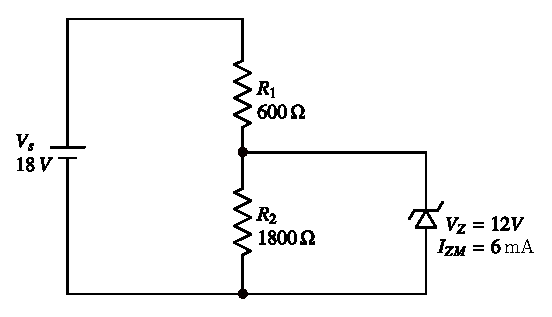
\includegraphics{chap2/exp2.29.eps}
\end{figure}
\end{example}

\begin{solution}
First let us calculate the voltage across $R_{2}$, by removing the Zener diode from the circuit.
\begin{figure}[H]
\centering
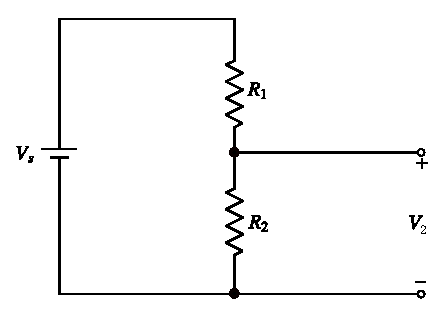
\includegraphics{chap2/sol2.29a.eps}
\end{figure}

Applying voltage division rule, we have
\begin{align*}
V_{2} &= \dfrac{V_{s}\,R_{2}}{R_{1}+R_{2}}=\dfrac{(18\text{\,V})(1800\,\Omega)}{600\,\Omega+1800\,\Omega}\\[5pt]
&= 13.5\text{\,V}
\end{align*}

Since, $V_{2}>V_{Z}$, the Zener diode operates in the breakdown region with a constant voltage of $V_{Z}=12\text{\,V}$, across it. Let us redraw the circuit with Zener diode connected across $R_{2}$.
\begin{figure}[H]
\centering
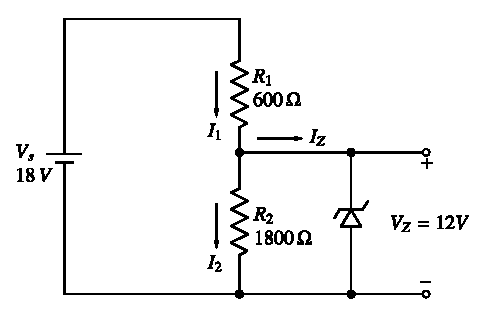
\includegraphics{chap2/sol2.29b.eps}
\end{figure}
\begin{align*}
I_{1} &= \dfrac{V_{S}-V_{Z}}{R_{1}}=\dfrac{18\text{\,V}-12\text{\,V}}{600\Omega}\\[4pt]
&= 10\text{\,mA}\\[4pt]
I_{2} &= \dfrac{V_{Z}}{R_{2}}=\dfrac{12\text{\,V}}{1800\Omega}\\[4pt]
&= 6.67\text{\,mA}\\[4pt]
I_{1} &= I_{2}+I_{Z}\\[4pt]
\text{or}\qquad I_{Z} &= I_{1}-I_{2}=10\text{\,mA}-6.67\text{\,mA}\\[4pt]
I_{Z} &= 3.33\text{\,mA}<I_{ZM}
\end{align*}
The Zener diode operates safely.

For the given values of $V_{S}$, $R_{1}$ and $R_{2}$ the circuit works as a voltage regulator.

But if $R_{2}$ is removed, all of $I_{1}$ flows into the Zener diode. As a result,
$$
I_{Z}=I_{1}=10\text{\,mA}>I_{ZM}
$$
This current will destroy the Zener diode.
\end{solution}

\begin{example}\label{exam2.32}
For the Zener diode network shown determine the following.
\begin{itemize}
\item[(a)] Load voltage, $V_{o}$

\item[(b)] Voltage across $R_{1}$, $V_{R_{1}}$

\item[(c)] Zener current, $I_{Z}$

\item[(d)] Zener dissipation, $P_{D}$
\end{itemize}

Take $V_{Z}=10\text{\,V}$ and $P_{D}=30\text{\,mW}$.
\begin{figure}[H]
\centering
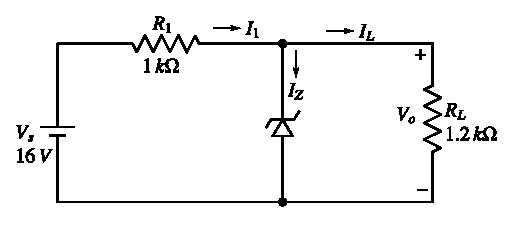
\includegraphics{chap2/exp2.30.eps}
\end{figure}
\end{example}

\begin{solution}
Let us find the voltage across $R_{L}$ by removing the Zener diode from the circuit.
\begin{figure}[H]
\centering
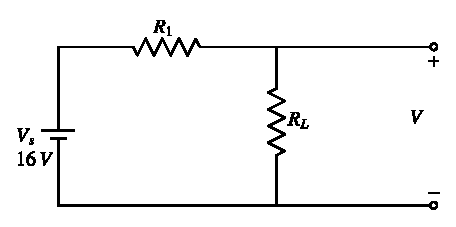
\includegraphics{chap2/sol2.30.eps}
\end{figure}

Using voltage division rule we have
\begin{align*}
V &= \dfrac{V_{S}R_{L}}{R_{1}+R_{L}}=\dfrac{16\text{\,V}\times 1.2\, k\Omega}{1k\Omega+1.2\,k\Omega}\\
&= 8.73\text{\,V}
\end{align*}

Note that, $V<V_{Z}$.

Therefore the Zener diode is in the off state. \ Hence \ $V_{0}=V=8.73V$.

Hence, $I_{Z}=0$, and $P_{D}=V_{Z}I_{Z}=0\text{\,W}$.

Writing KVL equation around the circuit, we have
\begin{align*}
V_{s} &= V_{R_{1}}+V\\[2pt]
V_{R_{1}} &= V_{s}-V=16\text{\,V}-8.73\text{\,V}\\[2pt]
&= 7.27\text{\,V}
\end{align*}
\vskip -1cm
\end{solution}

\begin{example}\label{exam2.33}
Repeat the previous example taking, $R_{L}=3\,k\Omega$.
\end{example}

\begin{solution}
With Zener diode removed, voltage across $R_{L}$ is given by,
$$
V=\dfrac{V_{s}\,R_{L}}{R_{1}+R_{2}}=\dfrac{16\text{\,V}\times 3\,k\Omega}{1k\Omega+3\,k\Omega}=12\text{\,V}
$$

Since, $V>V_{Z}$, the Zener diode operates in the breakdown region and has a constant voltage $V_{Z}=10\text{\,V}$ across it.

The circuit with Zener diode connected back is shown below.
\begin{figure}[H]
\centering
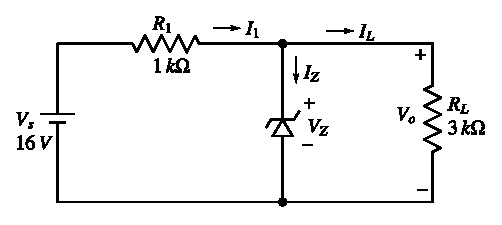
\includegraphics{chap2/sol2.31.eps}
\end{figure}
\vskip -.7cm
\begin{align*}
V_{o} &= V_{Z}=10\text{\,V}\\[3pt]
I_{L} &= \dfrac{V_{o}}{R_{L}}=\dfrac{10\text{\,V}}{3\,k\Omega}\\[3pt]
&= 3.33\text{\,mA}\\[3pt]
I_{1} &= \dfrac{V_{s}-V_{Z}}{R_{1}}=\dfrac{16\text{\,V}-10\text{\,V}}{1k\Omega}\\
&= 6\text{\,mA}\\[4pt]
V_{R_1} &= I_{1}R_{1}=(6\mA)(1\text{\,K\,}\Omega)\\
&= 6V\\
\text{Alternatively,}\quad V_{S} &= V_{R_{1}}+V_{Z}\\
\Rightarrow\quad V_{R_{1}} &= V_{S}-V_{Z}=16V-10V\\
&= 6V \\[5pt]
I_{ZM} &= \dfrac{P_{D}}{V_{Z}}=\dfrac{30\text{\,mW}}{10\text{\,V}}\\[4pt]
&= 3\text{\,mA}\\[4pt]
I_{Z} &= I_{1}-I_{L}=6\text{\,mA}-3.33\text{\,mA}\\[4pt]
&= 2.67\text{\,mA}
\end{align*}
Note that, $I_{Z}<I_{ZM}$
$$
P_{Z}=V_{Z}I_{Z}=(10\text{\,V})(2.67\text{\,mA})=26.7\text{\,mW}<30\text{\,mW}
$$
\vskip -.8cm
\end{solution}

\begin{example}\label{addexam2.34}
Design a Zener diode voltage regulator to meet the following requirements.
\begin{quote}
$dc$ input voltage : $10V\pm 20\%$

$dc$ output voltage : $5V$

load current : 20\,mA

Zener wattage : 400\,mW
\end{quote}
\end{example}

\begin{solution}
\begin{align*}
20\,\%~~\text{of}~~ 10V &= \frac{20}{100}\times 10V=2V\\[3pt]
\therefore\quad V_{S\max} &= 10V+2V=12V\\[3pt]
\text{and~ } V_{S\min} &= 10V-2V=8V\\[3pt]
V_{0}=5V &\Rightarrow V_{Z}=5V\\[3pt]
I_{Z_{M}} &=\frac{P_{D}}{V_{Z}}=\dfrac{400\text{\,mW}}{5V}\\[3pt]
&= 80\mA\\[3pt]
I_{1} &= I_{Z}+I_{L}\\[3pt]
\Rightarrow\quad I_{Z} &= I_{1}-I_{L}\tag{A}\\[3pt]
I_{1} &= \frac{V_{S}-V_{Z}}{R_{1}}\tag{B}
\end{align*}
using equation~(B) in equation~(A), we have
\begin{equation*}
I_{Z}=\dfrac{V_{S}-V_{Z}}{R_{1}}-I_{L}\tag{C}
\end{equation*}
When $V_{S}=V_{S\min}$ and $I_{L}=I_{L\max}$, $I_{Z}$ is minimum. From equation~(C), we have the following condition.
\begin{equation*}
\frac{V_{S\min}-V_{Z}}{R_{1}}-I_{L\max}>I_{Z_{K}}\tag{D}
\end{equation*}
($I_{Z}>I_{Z_{K}}$ ensures minimum reverse current to sustain breakdown)

Taking $I_{Z_{K}}=5\mA$ (Typical), we have
\begin{align*}
& \frac{8V-5V}{R_{1}}-20\mA>5\mA\\[2pt]
& \frac{3V}{R_{1}}>25\mA\\[2pt]
\Rightarrow\qquad & R_{1}<\frac{3V}{25\mA}\\[2pt]
\text{or}\qquad & \text{\fbox{$R_{1}<120\,\Omega$}}\tag{E}
\end{align*}
When $V_{S}=V_{S\max}$ and $I_{L}=0$, $I_{Z}$ is maximum. Again from equation~(C), we have the following condition.
\begin{equation}
\frac{V_{S\max}-V_{Z}}{R_{1}}<I_{Z_{M}}\tag{F}
\end{equation}
($I_{Z}<I_{Z_{M}}$, ensures safe operation of Zener diode)
\begin{align*}
& \frac{12V-5V}{R_{1}}<80\mA\quad\text{or}\quad \frac{7\V}{R_{1}}<80\mA\\[3pt]
& R_{1}>\frac{7V}{80\mA}\\[2pt]
& \text{\fbox{$R_{1}>87.5\,\Omega$}}\tag{G}
\end{align*}
Combining equations~(E) and (G), we have
$$
87.5\,\Omega < R_{1}<120\,\Omega
$$

Taking the average of the two values, we get
\begin{align*}
R_{1} &= \frac{87.5\,\Omega+120\,\Omega}{2}=103.75\,\Omega\\
R_{L} &= \frac{V_{0}}{I_{L}}=\frac{5V}{20\mA}\\
     &= 250\,\Omega
\end{align*}

\eject

The required circuit is shown below.
\begin{figure}[H]
\centering
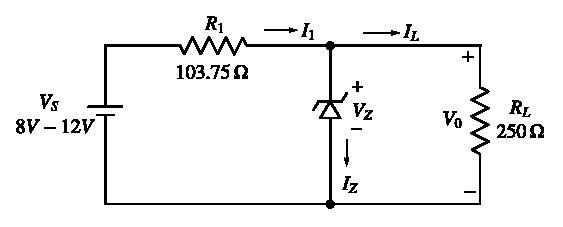
\includegraphics{chap2/newfig1.eps}
\end{figure}
\vskip -.9cm
\end{solution}

\begin{example}\label{exam2.34}
For a Zener diode regulator, derive the expressions for
\begin{itemize}
\itemsep=0pt
\item[(a)] Source effect and line regulation

\item[(b)] Ripple rejection ratio

\item[(c)] Output resistance

\item[(d)] Load effect and load regulation
\end{itemize}
\end{example}

\begin{solution}
\begin{itemize}
\item[(a)] {\bf Source effect and line regulation}

Let $\Delta V_{o}$ be the change in the output voltage when the input voltage changes by $\Delta V_{i}$. When the voltages are changing the Zener diode can be replaced by its dynamic impedance $Z_{Z}$ as shown in Fig.~A.
\begin{figure}[H]
\centering
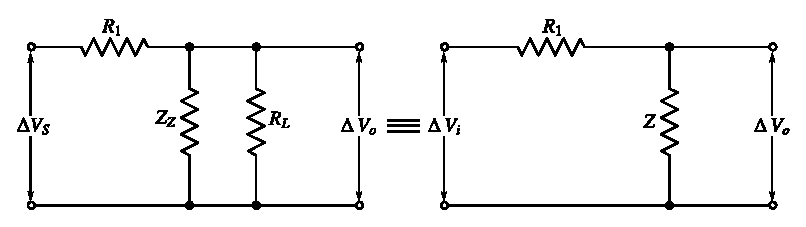
\includegraphics{chap2/figA.eps}

\bigskip
\colorbox{lightgray}{{\bf Fig.~A~:} \em Dynamic equivalent circuit of Zener voltage regulator}
\end{figure}
\vskip -.8cm
\begin{equation*}
Z=Z_{Z}\,||\,R_{L}\tag{A}
\end{equation*}
Using voltage division rule,
\begin{align*}
\Delta V_{o} &= \left(\dfrac{\Delta V_{S}}{R_{1}+Z}\right)Z\\[4pt]
\Delta V_{o} &= \dfrac{\Delta V_{S}[Z_{Z}\,||\,R_{L}]}{R_{1}+[Z_{Z}\,||\,R_{L}]}\tag{B}
\end{align*}
Under no load i.e., without $R_{L}$, $Z=Z_{Z}$
\begin{equation}
\text{Now,}\qquad \Delta V_{o} =\dfrac{\Delta V_{S}\,Z_{Z}}{R+Z_{Z}}\tag{C}
\end{equation}
Using Eqns.~(B) and (C) we can find the source effect for the regulator with load and without load (i.e., no load) respectively.
\begin{equation*}
\text{Line regulation } = \dfrac{(\Delta V_{o}\text{~ for~ } 10\%\text{~ change in~ } V_{S})}{V_{S}}\times 100\%\tag{D}
\end{equation*}

\item[(b)]\hfill Ripple rejection ratio = $\dfrac{V_{r_o}}{V_{r_i}}$\hfill (E)

$V_{r_o}$ is the ripple voltage at the regulator output.

$V_{r_i}$ is the ripple voltage at the regulator input.

Fig.~B shows the dynamic equivalent circuit of regulator with $V_{r_i}$ and $V_{r_o}$ indicated.
\begin{figure}[H]
\centering
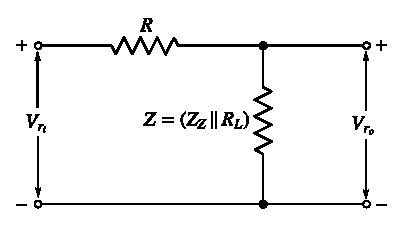
\includegraphics{chap2/figB.eps}

\bigskip
\colorbox{lightgray}{{\bf Fig.~B~:} \em Dynamic equivalent circuit with ripple voltages}
\end{figure}

Using voltage division rule,
\begin{align*}
V_{r_o} &=\left(\dfrac{V_{r_i}}{R+Z}\right)Z\\[4pt]
\dfrac{V_{r_o}}{V_{r_i}} &= \dfrac{Z}{R+Z}=\dfrac{(Z_{Z}\,||\,R_{L})}{R+(Z_{Z}\,||\,R_{L})}\tag{F}
\end{align*}

\item[(c)] {\bf Output resistance \boldmath$R_{o}$.}

Consider the dynamic equivalent circuit shown in Fig.~A.
\begin{itemize}
\item[(i)] Short circuit the input terminals.

\item[(ii)] Remove $R_{L}$.
\end{itemize}

The equivalent resistance measured between the output terminals is the output resistance $R_{o}$. This is illustrated in Fig.~C.
\begin{figure}[H]
\centering
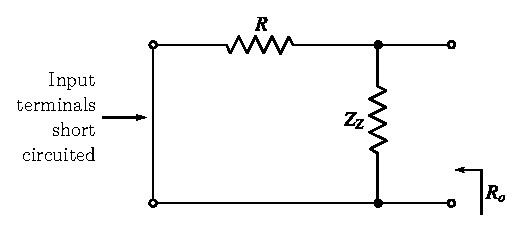
\includegraphics{chap2/figC.eps}

\bigskip
\colorbox{lightgray}{{\bf Fig.~C~:} \em Equivalent circuit to find $R_{O}$}
\end{figure}

As seen from the output terminals, $R$ and $Z_{Z}$ are in parallel
\begin{equation*}
\therefore\quad R_{o}=R\;||\;Z_{Z}=\dfrac{R\,R_{Z}}{R+R_{Z}}\tag{G}
\end{equation*}

\item[(d)] {\bf Load effect and load regulation.}

The voltage source representation of Zener regulator can be obtained by placing $R_{o}$ in series with the voltage source $V_{o}$ as shown in Fig.~D.
\begin{figure}[H]
\centering
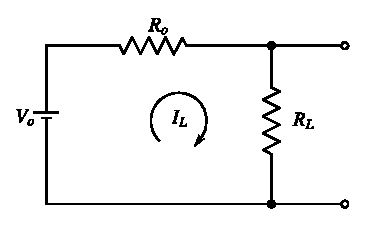
\includegraphics{chap2/figD.eps}

\bigskip
\colorbox{lightgray}{{\bf Fig.~D~:} \em Voltage source representation of Zener regulator}
\end{figure}
\vskip -.8cm
\begin{equation*}
V_{o}=\text{~voltage across~ $R_{o}+$ load voltage = constant}\tag{H}
\end{equation*}

When the load current increases by $\Delta I_{L}$, the voltage across $R_{o}$ increases by $R_{o}\,\Delta I_{L}$ and the load voltage decreases by the same amount (see Eqn.~(H)).
\begin{align*}
\therefore\quad \text{Output voltage change, } \Delta V_{o} &= R_{o}\,\Delta I_{L}= [Z_{Z}\,||\,R_{L}]\,\Delta I_{L}\\[4pt]
\text{load regulation} &= \dfrac{\Delta V_{o}\text{~~ for~~ } \Delta L_{L(\max)}}{V_{o}}\times 100\,\%
\end{align*}
\end{itemize}
\vskip -1cm
\end{solution}

\eject

\noindent
{\bf Note~:} 
Line regulation, load regulation, output resistance and ripple rejection ratio are called the performance parameters of a regulator.

\begin{example}\label{exam2.35}
A Zener regulator has the following data:
\begin{align*}
V_{S} &= 16\text{\,V}\\[3pt]
V_{o} &= 6\text{\,V}\\[3pt]
I_{L_{\max}} &= 60\text{\,mA}\\[3pt]
Z_{Z} &= 7\Omega\\[3pt]
R &= 150\Omega
\end{align*}
Calculate the line regulation, output resistance, load regulation and ripple rejection ratio.
\end{example}

\begin{solution}
Source effect
\begin{align*}
\Delta V_{S} &= 10\%\text{~~ of~~ } V_{S}\\[4pt]
&= 10\%\text{~~ of~~ }16V\\[4pt]
&= 1.6\text{\,V}\\[4pt]
R_{L} &= \dfrac{V_{o}}{I_{L}}=\dfrac{6\text{\,V}}{60\text{\,mA}}=100\,\Omega\\[4pt]
Z_{Z}\,||\,R_{L} &= \dfrac{7\,\Omega\times 100\,\Omega}{7\,\Omega+100\,\Omega}=6.54\,\Omega\\[4pt]
\Delta V_{o} &= \dfrac{\Delta V_{S}[Z_{L}\,||\,R_{L}]}{R+[Z_{Z}\,||\,R_{L}]}=\dfrac{1.6\V\times 6.54\,\Omega}{150\,\Omega+6.54\,\Omega}=66.84\text{\,mV}\\[4pt]
\text{Line regulation} &= \dfrac{(\Delta V_{o}\text{~~ for~~ }10\%\text{~~ change in~~ } V_{S})}{V_{o}}\times 100\,\%\\[4pt]
&= \dfrac{66.84\text{\,mV}\times 100}{6\V}\\[4pt]
&= 1.114\,\%\\[4pt]
\text{Load effect}\quad \Delta V_{o} &= \Delta I_{L(\max)}[Z_{Z}\,||\,R]\\[4pt]
\Delta I_{L(\max)} &= I_{L_{\max}}-I_{L_{\min}}\\[4pt]
&= 60\text{\,mA}-0\text{\,mA}\\[4pt]
&= 60\text{\,mA}\\[4pt]
Z_{Z}\,||\,R &= \dfrac{7\,\Omega\times 150\,\Omega}{7\,\Omega+150\,\Omega}=6.69\,\Omega\\[4pt]
\Delta V_{o} &= (60\,\text{mV})(6.68)\\[4pt]
&= 400\text{\,mV}\\[4pt]
\text{output resistance,}~~~ R_{o} &= Z_{Z}\,||\,R\\[4pt]
&= 6.69\,\Omega\\[4pt]
\text{Ripple rejection ratio,}\quad \dfrac{V_{r_o}}{V_{r_i}} &= \dfrac{Z_{Z}\,||\,R_{L}}{R+Z_{Z}\,||\,R_{L}}\\[4pt]
&= \dfrac{6.54\,\Omega}{150\,\Omega+6.54\,\Omega}\\[2pt]
&= 0.0418
\end{align*}
\vskip -1cm
\end{solution}

\section{Clipping Circuits}\label{sec2.29}

Clipping circuits are used to clip off an unwanted portion of a waveform. Clipping\index{Clipping} circuits are also called as limiting circuits. Limiting of either positive or negative amplitude in large amplitude signal is some times necessary to protect the devices or circuits which otherwise might get destroyed. Since, diode allows current in only one direction, it can be used in clipping circuits. Depending upon how the diode is placed in the circuit, We have the following two types of clipper.
\begin{enumerate}
\item Series clipper\index{Clipping!series}

\item Shunt clipper
\end{enumerate}

In series clipper, the diode appears as a series element and in a shunt clipper the diode appears in parallel with the output terminals or the load.

\section{Series Clipper}\label{sec2.30}

A halfwave rectifier can be considered as a clipper because it passes only half cycle and clips off the other half cycle of the applied input. Therefore a series clipper is essentially a halfwave rectifier circuit.

\subsection{Negative series clipper}\label{sec2.30.1}
\index{Negative series clipper}

Fig.~\ref{fig2.25} shows the circuit of negative series clipper\index{Clipping!negative series clipper} along with input and output waveforms. Note that the circuit operates without $R_{L}$. Hence the load current $I_{L}$ is zero.
\begin{figure}[H]
\centering
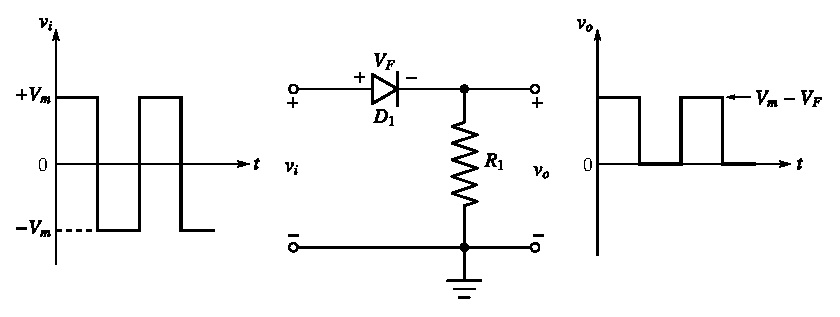
\includegraphics{chap2/fig2.25.eps}
\caption{Negative series clipper}\label{fig2.25}
\end{figure}

During the positive half cycle of input,
$$
v_{i}=V_{m}\,(>V_{F})
$$

$V_{F}$ is the forward bias voltage required for the diode to conduct. For a silicon diode, $V_{F}=0.7V$.

The diode conducts and the current flows into $R_{1}$.

Applying $KVL$ to the path consisting of $v_{i}$, $V_{F}$ and $v_{0}$ when the diode is conducting, we have
\begin{align}
& v_{i}-V_{F}-v_{0}=0\notag\\
& v_{0}=v_{i}-V_{F}\label{eq2.88}
\end{align}

Since, $v_{i}=V_{m}$, we have
\begin{equation}
v_{0}=V_{m}-V_{F}\label{eq2.89}
\end{equation}

Note that, the output voltage $v_{0}$ is less than the input voltage amplitude, $V_{m}$, by an amount $V_{F}$.

During the negative half cycle of input,
$$
v_{i}=-V_{m}\,(<V_{F})
$$

The diode is reverse biased and only the reverse saturation current, $I_{R}$, flows through $R_{1}$.
\begin{equation}
\text{Hence}\qquad v_{0}=-I_{R}\,R_{1}\label{eq2.90}
\end{equation}

Since, $I_{R}$ is very small,
\begin{equation}
v_{0}\approx 0\label{eq2.91}
\end{equation}

\heading{Summary}

{\em The circuit passes only positive half cycles and clips off the negative half cycles of $v_{i}$. Hence the name negative clipper.}

\subsection{Positive clipper}\label{sec2.30.2}
\index{Positive clipper}

Fig.~\ref{fig2.26} shows the circuit of positive clipper.\index{Clipping!positive clipper} This circuit is obtained by reversing the diode connection in negative clipper circuit.
\begin{figure}[H]
\centering
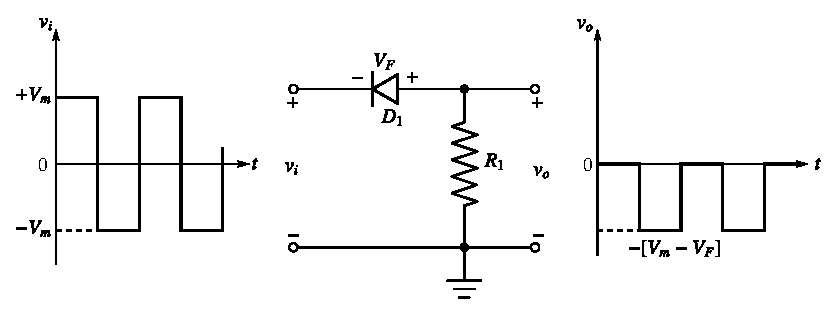
\includegraphics{chap2/fig2.26.eps}
\caption{Negative series clipper}\label{fig2.26}
\end{figure}

During the positive half cycle of input,
$$
v_{i}=V_{m}
$$

The diode is reverse biased and only the reverse saturation current $I_{R}$ of diode flows through~$R_{1}$.

Hence,
\begin{equation}
v_{0}=I_{R}\,R_{1}\approx 0\label{eq2.92}
\end{equation}

During the negative half cycle of input,
$$
v_{i}=-V_{m}
$$
The diode conducts and the current flows through $R_{1}$.

Applying $KVL$ to the path containing $v_{i}$, $V_{F}$ and $v_{0}$ we have,
\begin{equation}
v_{i}+V_{F}-v_{0}=0\label{eq2.93}
\end{equation}
using, $v_{i}=-V_{m}$ we have
\begin{equation}
v_{0}=-[V_{m}-V_{F}]\label{eq2.94}
\end{equation}

\heading{Summary}

{\em The circuit passes only negative half cycles and clips off the positive half cycles of $v_{i}$.}

{\em Hence the name positive clipper.}

\begin{example}\label{exam2.37}
For the negative series clipper with zero load current shown below find a suitable resistor $R_{1}$ and specify the diode forward current and reverse voltage, for a silicon diode. Sketch the output voltage waveform.
\begin{figure}[H]
\centering
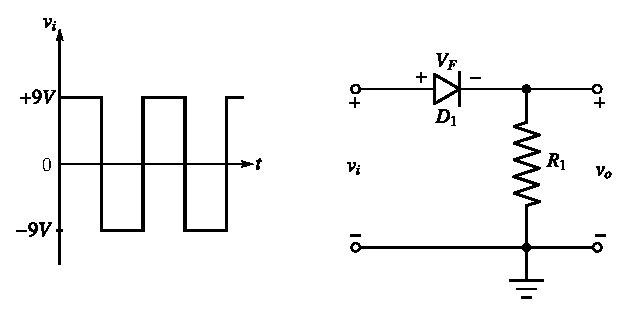
\includegraphics{chap2/exp2.37.eps}
\end{figure}
\end{example}

\begin{solution}
When the diode conducts,
\begin{align*}
v_{0} &= V_{m}-V_{F}\\[3pt]
     &= 9\V-0.7\V\\[3pt]
     &= 8.3\V
\end{align*}

The diode forward current, $I_{F}$, flows through $R_{1}$.
\begin{align*}
\therefore\quad v_{0} &= I_{F}\,R_{1}\\[3pt]
R_{1} &= \frac{v_{0}}{I_{F}}=\frac{8.3V}{I_{F}}
\end{align*}
Choose, $I_{F}=1\mA$ [which is sufficient to keep the diode in conduction]
$$
R_{1}=\frac{8.3V}{1\mA}=8.3\,k\Omega
$$

During negative half cycles of $v_{i}$, the diode is reverse biased by $-V_{m}$. Therefore the reverse voltage on diode is
$$
-V_{R}=-V_{m}=-9V\quad\Rightarrow\quad V_{R}=9V
$$

\eject

\heading{Diode Specification}
\begin{center}
\begin{minipage}[t]{5cm}
\vskip .5cm
\begin{flalign*}
&V_{R} = 9V&&\\[3pt]
&I_{F} = 1\mA&&
\end{flalign*}
\end{minipage}
\quad
\begin{minipage}[t]{5cm}
\begin{figure}[H]
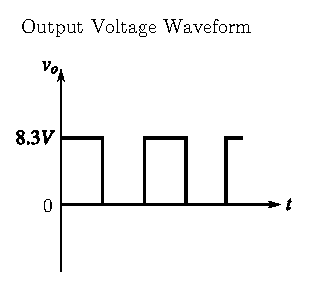
\includegraphics{chap2/sol2.37.eps}
\end{figure}
\end{minipage}
\end{center}
\vskip -.75cm
\end{solution}

\smallskip
\begin{example}\label{exam2.38}
A positive series clipping circuit has a $\pm 7V$ input and zero load current. Calculate a suitable resistor for $R_{1}$ and specify the diode. Sketch the output voltage waveform.
\end{example}

\begin{solution}
When the diode conducts,
$$
v_{0}=-[V_{m}-V_{F}]
$$
Assuming silicon diode
$$
V_{F}=0.7V
$$
Also, $V_{m}=7V$
\begin{align*}
\therefore\quad v_{0} &= -[7V-0.7V]\\[3pt]
&=-\,6.3V\\[3pt]
R_{1} &= \frac{v_{0}}{I_{F}}\\[3pt]
&= \frac{6.3V}{1\mA}\\[3pt]
&=6.3\,k\Omega\\[3pt]
V_{R} &= V_{m}=7V
\end{align*}
\heading{Diode Specification}
\begin{align*}
V_{R} &= 7V\\[4pt]
I_{F} &= 1\mA
\end{align*}

\eject

The positive series clipper along with input and output waveforms is shown below.
\begin{figure}[H]
\centering
\includegraphics{chap2/sol2.38.eps}
\end{figure}
\vskip -1cm
\end{solution}

\smallskip

\begin{example}\label{exam2.39}
A $\pm\, 6V$ square wave is applied via a series clipping circuit to a device that cannot survive $+6V$. The device input current is $100\,\mu \text{\,A}$ when the input voltage is negative. Select a suitable clipping circuit and calculate the value of $R_{1}$. Also specify the diode.
\end{example}

\begin{solution}
The device connected to the clipper cannot survive $+6V$. Therefore we have to clip off the positive half cycles of input. Hence a positive clipper is required. When the diode conducts,
\begin{align*}
v_{0} &= -[V_{m}-V_{F}]\\[3pt]
      &= -[6\V-0.7\V]\\[3pt]
&= -5.3V\quad\text{[Assuming silicon diode]}
\end{align*}
Diode current = current through $R_{1}+$ Device current
\begin{align*}
I_{F} &= 1\mA + 100\mu \text{\,A} = 1.1\mA\\[3pt]
R_{1} &= \frac{v_{0}}{I_{F}}=\frac{5.3V}{1.1\mA}=4.8\,k\Omega
\end{align*}
\heading{Diode Specification}
\begin{align*}
I_{F} &= 1.1\mA\\[3pt]
V_{R} &= 6V
\end{align*}

\eject

The circuit arrangement is shown below.
\begin{figure}[H]
\centering
\includegraphics[scale=.9]{chap2/sol2.39.eps}
\end{figure}
\vskip -1cm
\end{solution}

\subsection{Series noise clipper}\label{sec2.30.3}
\index{Series noise clipper}

Any unwanted signal is called the noise. Sometimes lower level noise voltage may be present in digital signal wave forms, which is unwanted. This noise voltage can be eliminated by a series noise clipping\index{Clipping!series noise clipping} circuit shown in Fig.~\ref{fig2.27}.
\begin{figure}[H]
\centering
\includegraphics[scale=.9]{chap2/fig2.27.eps}
\caption{Series noise clipping circuit}\label{fig2.27}
\end{figure}

The circuit contains two diodes connected in anti-parallel. For the circuit to work properly:
\begin{itemize}
\item[$\bullet$] the noise amplitude must be much smaller than the diode forward voltage, $V_{F}$.

\item[$\bullet$] the peak signal amplitude $V_{m}$ must be larger than the doide forward voltage, $V_{F}$.
\end{itemize}

Under this condition, the diodes conduct only the signal part and blocks the noise. The peak output voltage is $V_{m}-V_{F}$, where $V_{m}$ is the peak value of input voltage.

For, $-V_{F}<v_{i}<V_{F}$, none of the diodes conduct and the output voltage is zero. This range of input voltage during which the output voltage is zero is called the dead zone.

If the noise amplitude exceeds $\pm V_{F}$, two diodes may be connected in series to provide a larger dead zone.

\vfill\eject

\section{Shunt Clipping Circuits}\label{sec2.31}
\index{Clipping!shunt}

In shunt clipper, the diode is connected in parallel with the output terminals.

\vskip .1cm
As in the case of series clipper, we have positive and negative shunt clippers.

\subsection{Positive shunt clipper}\label{sec2.31.1}

Fig.~\ref{fig2.28} shows the circuit of positive shunt clipper.\index{Positive shunt clipper} Note that the diode is connected in shunt or parallel with the load $R_{L}$.
\setcounter{figure}{27}
\begin{figure}[H]
\centering
\includegraphics{chap2/fig2.28.eps}
\caption{Positive shunt clipper}\label{fig2.28}
\end{figure}

During the positive half cycle of input, $v_{i}=V_{m}$. The diode conducts and the equivalent circuit is shown in Fig.~\ref{fig2.29}.
\begin{figure}[H]
\centering
\includegraphics{chap2/fig2.29.eps}
\caption{Equivalent circuit when the diode conducts}\label{fig2.29}
\end{figure}

Since the diode and $R_{L}$ are in parallel.
\begin{equation}
v_{0}=V_{F}\label{eq2.95}
\end{equation}

Note that, $v_{0}$ is very small. Hence $I_{L}$ is also small $(\because~ v_{0}=I_{L}\,R_{L})$.

$\Rightarrow$\quad {\em The circuit clips off positive half cycles of input.}
\begin{align}
\text{Also,}\quad I_{1} &= I_{F}+I_{L}\label{eq2.96}\\[4pt]
\text{Since,}\quad I_{L} &\ll I_{F},\quad\text{we have}\notag\\[4pt]
I_{1} &\approx I_{F}\label{eq2.97}
\end{align}

Applying $KVL$ to the path consisting of $v_{i}$, $R_{1}$ and $D_{1}$, we have
\begin{equation}
V_{m}-I_{1}R_{1}-V_{F}=0\label{eq2.98}
\end{equation}

Since, $I_{1}\approx I_{F}$, we have
\begin{equation}
I_{F}=\frac{V_{m}-V_{F}}{R_{1}}\label{eq2.99}
\end{equation}

During the negative half cycle of input, $v_{i}=-V_{m}$. The diode is reverse biased and the equivalent circuit is shown in Fig.~\ref{fig2.30}.
\begin{figure}[H]
\centering
\includegraphics[scale=1.1]{chap2/fig2.30.eps}
\caption{Equivalent circuit when the diode is non conducting}\label{fig2.30}
\end{figure}

Notice the change in current directions
\begin{align}
& I_{1}=I_{R}+I_{L}\notag\\[3pt]
\text{Since,}\quad & I_{R}\ll I_{L}\notag\\[3pt]
& I_{1}\approx I_{L}\label{eq2.100}
\end{align}

Applying $KVL$ to the path consisting of $v_{i}$, $R_{1}$ and $R_{L}$, we have
$$
v_{i}+I_{1}R_{1}-v_{0}=0
$$
using $v_{i}=-V_{m}$, and $I_{1}\approx I_{L}$, we get
\begin{equation}
v_{0}=-[V_{m}-I_{L}\,R_{1}]\label{eq2.101}
\end{equation}

Note that, the output voltage is negative and its peak level is less than $V_{m}$ by an amount $I_{L}\,R_{1}$.

$\Rightarrow$\quad {\em The circuit passes negative half cycles of input to the output.}

From Eqn.~\eqref{eq2.101}.
\begin{equation}
R_{1}=\frac{v_{0}+V_{m}}{I_{L}}\label{eq2.102}
\end{equation}

It is important to note that, $v_{0}$ is negative and $|v_{0}|<V_{m}$. Hence $R_{1}$ is positive.

\medskip

\heading{Summary}

{\em A positive shunt clipper clips off the positive half cycles of $v_{i}$ and passes only the negative half cycles to the output.}

\subsection{Design equations of positive shunt clipper}\label{sec2.31.2}
\index{Positive shunt clipper}

When the diode is conducting:
\begin{align}
v_{0} &= V_{F}\label{eq2.103}\\[4pt]
I_{F} &= \frac{V_{m}-V_{F}}{R_{1}}\label{eq2.104}
\end{align}
when the diode is non-conducting:
\begin{align}
v_{0} &= -[V_{m}-I_{L}R_{1}]\label{eq2.105}\\[4pt]
R_{1} &= \frac{v_{0}+V_{m}}{I_{L}}\label{eq2.106}\\[4pt]
V_{R} &= V_{m}\label{eq2.107}
\end{align}

\eject
\subsection{Negative shunt clipper}\label{sec2.31.3}
\index{Clipping!negative shunt clipper}

Negative shunt clipper\index{Negative shunt clipper} is obtained by reversing the diode connection in the circuit of positive shunt clipper, as shown in Fig.~\ref{fig2.31}.
\begin{figure}[H]
\centering
\includegraphics{chap2/fig2.31.eps}
\caption{Negative shunt clipper}\label{fig2.31}
\end{figure}

During the positive half cycle of input, $v_{i}=V_{m}$. The diode is reverse biased and the equivalent circuit is shown in Fig.~\ref{fig2.32}.
\begin{figure}[H]
\centering
\includegraphics{chap2/fig2.32.eps}
\caption{Equivalent circuit when the diode is non conducting}\label{fig2.32}
\end{figure}
\vskip -.8cm
\begin{equation}
I_{1}=I_{R}+I_{L}\label{eq2.108}
\end{equation}
Since, $I_{R}\ll I_{L}$
\begin{equation}
I_{1}\approx I_{L}\label{eq2.109}
\end{equation}

Applying $KVL$ to the path consisting of $v_{i}$, $R_{1}$ and $R_{L}$ we have
\begin{equation}
v_{i}-I_{1}R_{1}-v_{0}=0\label{eq2.110}
\end{equation}
using, $v_{i}=V_{m}$ and $I_{1}=I_{L}$, we have
\begin{align}
& V_{m}-I_{L}\,R_{1}-v_{0}=0\label{eq2.111}\\
& v_{0}=V_{m}-I_{L}R_{1}\label{eq2.112}
\end{align}

Note that, the output voltage is positive and its peak level is less than $V_{m}$ by an amount $I_{L}\,R_{1}$.

$\Rightarrow$\quad {\em The circuit passes positive half cycles of input to the output.}

Also, from Eqn.~\eqref{eq2.112},
\begin{equation}
R_{1}=\frac{V_{m}-v_{0}}{I_{L}}\label{eq2.113}
\end{equation}

During the negative half cycle of input, $v_{i}=-V_{m}$. The diode conducts and the equivalent circuit is shown in Fig.~\ref{fig2.33}.
\begin{figure}[H]
\centering
\includegraphics{chap2/fig2.33.eps}
\caption{Equivalent circuit when the diode is conducting}\label{fig2.33}
\end{figure}

Since the diode and $R_{L}$ are in parallel.
\begin{equation}
v_{0}=-V_{F}\label{eq2.114}
\end{equation}

The negative sign is due to the fact that, polarities of $V_{F}$ and $v_{0}$ are opposite.

Note that, $v_{0}$ is very small. Hence $I_{L}$ is also small.

$\Rightarrow$\quad {\em The circuit clips off negative half cycles of input}
\begin{align}
\text{Also,}\quad & I_{1}=I_{F}+I_{L}\label{eq2.115}\\[3pt]
\text{Since,}\quad & I_{L}\ll I_{F}\notag\\[3pt]
& I_{I}\approx I_{F}\label{eq2.116}
\end{align}

Applying $KVL$ to the path consisting of $v_{i}$, $R_{1}$ and $D_{1}$ we have,
\begin{equation}
v_{i}+I_{1}R_{1}+V_{F}=0\label{eq2.117}
\end{equation}
using, $v_{i}=-V_{m}$, and $I_{1}=I_{F}$ we get
\begin{equation}
I_{F}=\dfrac{V_{m}-V_{F}}{R_{1}}\label{eq2.118}
\end{equation}

\heading{Summary}

{\em A negative shunt clipper clips off the negative half cycles of $v_{i}$ and passes only the positive half cycles to the output.}

\subsection{Design equations of negative shunt clipper}\label{sec2.31.4}

When the diode is non conducting~:
\begin{align}
& v_{0}=V_{m}-I_{L}\,R_{1}\label{eq2.119}\\
& R_{1}=\dfrac{V_{m}-v_{0}}{I_{L}}\label{eq2.120}\\
& V_{R}=V_{m}\label{eq2.121}
\end{align}
when the diode is conducting~:
\begin{align}
& v_{0} =-V_{F}\label{eq2.122}\\
& I_{F}=\frac{V_{m}-V_{F}}{R_{1}}\label{eq2.123}
\end{align}

\noindent
{\bf Note:~} The reader is advised to compare the design equations of positive and negative shunt clippers and note down the differences.

\begin{example}\label{exam2.40}
The negative shunt clipper of Fig.~\ref{fig2.31} has a $\pm 8V$ input, and is to produce a $+7.5V$ output when the load current is $2\mA$. Find a suitable value for $R_{1}$ and specify the diode forward current and reverse voltage.
\end{example}

\begin{solution}
Given
\begin{align*}
V_{m} &= 8V\\
v_{0} &=7.5V\quad I_{L}=2\mA
\end{align*}
Refer the design equations of negative shunt clipper. 

When the diode is not conducting~:
\begin{align*}
R_{1} &= \frac{V_{m}-v_{0}}{I_{L}}=\frac{8V-7.5V}{2\mA}\\[3pt]
&= 250\Omega
\end{align*}
Diode reverse voltage:
$$
V_{R}=V_{m}=8V
$$
when the diode is conducting:
\begin{align*}
I_{F} &= \frac{V_{m}-V_{F}}{R_{1}}=\frac{8V-0.7V}{250\,\Omega}\\[3pt]
&= 29.2\mA\\[3pt]
v_{0} &= -V_{F}=-0.7V
\end{align*}

The circuit of negative shunt clipper along with input and output waveforms is shown below.
\begin{figure}[H]
\centering
\includegraphics{chap2/sol2.40.eps}
\end{figure}
\end{solution}

\begin{example}\label{exam2.41}
A positive shunt clipper of Fig.~\ref{fig2.28}, has $\pm 7V$ input. The output voltage is to be $-6.5V$ when the load current is $2\mA$. Calculate the value for $R_{1}$ and specify the diode forward current and reverse voltage.
\end{example}

\begin{solution}
Given,
\begin{align*}
V_{m} &= 7V\\[3pt]
v_{0} &= -\,6.5V\qquad I_{L}=2\mA
\end{align*}

Refer the design equations of positive shunt clipper, when the diode is not conducting:
\begin{align*}
R_{1} &= \frac{v_{0}+V_{m}}{I_{L}}=\dfrac{-6.5V+7V}{2\mA}\\[3pt]
&= 250\Omega
\end{align*}

Diode reverse voltage:
$$
V_{R}=V_{m}=7V
$$
when the diode is conducting:
\begin{align*}
v_{0} &= V_{F}=0.7V\\[3pt]
I_{F} &= \frac{V_{m}-V_{F}}{R_{1}}=\frac{7V-0.7V}{250\,\Omega}\\[3pt]
&= 25.2\mA
\end{align*}

The circuit of positive shunt clipper along with input and output waveforms is shown below.
\begin{figure}[H]
\centering
\includegraphics{chap2/sol2.41.eps}
\end{figure}
\end{solution}

\begin{example}\label{exam2.42}
A device is to be protected from the negative half cycle of a $\pm\,6V$ square wave input. The device current is $750\,\mu\text{A}$ when its input is $+\,4V$. Select a suitable shunt clipping circuit. Find the resistor value and specify the diode.
\end{example}

\begin{solution}
Given
$$
V_{m}=6V
$$

The device is nothing but a load connected to shunt clipper.

Load current = Device current

$\therefore$~~ $I_{L}=750\,\mu\text{A}=0.75\mA$ at $v_{0}=4V$.

In order to protect the device from negative half cycles, a negative shunt clipper is to be used.

When the diode is not conducting.
\begin{align*}
R_{1} &= \frac{V_{m}-v_{0}}{I_{L}}=\frac{6V-4V}{0.75\mA}\\[3pt]
&= 2.67k\Omega
\end{align*}

Diode reverse voltage:
$$
V_{R}=V_{m}=6V
$$
when the diode is conducting:
\begin{align*}
v_{0} &= -V_{F}=-0.7V\\[3pt]
I_{F} &= \frac{V_{m}-V_{F}}{R_{1}}=\frac{6V-0.7V}{2.67k\Omega}\\[3pt]
&= 1.98\mA
\end{align*}

The circuit of negative shunt clipper along with input and output wave forms is shown below.
\begin{figure}[H]
\centering
\includegraphics{chap2/sol2.42.eps}
\end{figure}
\end{solution}

\begin{example}\label{exam2.43}
For the circuits shown in Fig.~(a) and (b), the input is a square wave of $\pm 10V$ amplitude. Sketch the output voltage wave form for both the circuits.
\begin{figure}[H]
\centering
\includegraphics{chap2/exp2.43.eps}
\end{figure}
\end{example}

\begin{solution}
The circuit of Fig.~(a) is a positive shunt clipper without $R_{L}$. Hence the load current, $I_{L}=0$.

Refer the design equations of positive shunt clipper.

When the diode conducts:
$$
v_{0}=V_{F}=0.7V
$$
when the diode is not conducting:
$$
R_{1}=\dfrac{V_{m}+v_{0}}{I_{L}}\quad\Rightarrow\quad v_{0}=-V_{m}+I_{L}R_{1}
$$
Since, $I_{L}=0$
$$
v_{0}=-V_{m}=-10V
$$

The input and output voltage wave forms are given below
\begin{figure}[H]
\centering
\includegraphics{chap2/sol2.43a.eps}
\end{figure}

The circuit of Fig.~(b) is a negative shunt clipper without $R_{L}$. Hence, $I_{L}=0$.

Refer the design equations of negative shunt clipper.

When the diode is conducting:
$$
v_{0}=-V_{F}=-0.7V
$$
When the diode is not conducing:
$$
R_{1}=\frac{V_{m}-v_{0}}{I_{L}}\quad\Rightarrow\quad v_{0}=V_{m}-I_{L}R_{L}
$$
Since, $I_{L}=0$
$$
v_{0}=V_{m}=10V
$$
The input and output voltage wave forms are shown below
\begin{figure}[H]
\centering
\includegraphics{chap2/sol2.43b.eps}
\end{figure}
\vskip -1cm
\end{solution}

\eject

\subsection{Shunt noise clipper}\label{sec2.31.5}
\index{Clipping!shunt noise clipper}

Fig.~\ref{fig2.34} shows the circuit of shunt noise clipper.\index{Shunt noise clipper} It consists of diodes connected in antiparallel between the output terminals. Shunt noise clipper is used to remove the noise riding on the peaks of an input waveform.
\begin{figure}[H]
\centering
\includegraphics[scale=.97]{chap2/fig2.34.eps}
\caption{Shunt noise clipper}\label{fig2.34}
\end{figure}

The signal amplitude must be greater than the diode forward voltage drop, $V_{F}$. During the positive half cycle of input, $D_{1}$ conducts and limits the output at, $+V_{F}$. During the negative half cycle of input, $D_{2}$ conducts and limits the output at, $-V_{F}$.\\[-20pt]

\subsection{Application of shunt clipper}\label{sec2.31.6}

Pulse width modulation is a type of modulation in communication system, where in the information is made to contain in the width of a pulse waveform. During transmission the noise rides on the peaks of pulse and corrupts the pulse waveform. 

Shunt clipper is used to clip-off the noise riding on the peaks of pulse waveform. Since the information is contained in the pulse width, removal of corrupted amplitude does not affect the information.\\[-20pt]

\section{Biased shunt clipper}\label{sec2.32}

Fig.~\ref{fig2.35} shows the circuit of biased shunt clipper.
\begin{itemize}
\itemsep=0pt
\item[$\bullet$] Diodes $D_{1}$ and $D_{2}$ are both reverse biased by $V_{B}$.

\item[$\bullet$] When $v_{i}\geq V_{B}+V_{F}$, $D_{1}$ conducts and $D_{2}$ is reverse biased.

Thus $v_{0}=V_{F}+V_{B}$.

\item[$\bullet$] When $v_{i}\leq -(V_{B}+V_{F})$, $D_{2}$ conducts and $D_{1}$ is reverse biased.

Thus $v_{0}=-(V_{B}+V_{F})$.

\item[$\bullet$] For \, $-(V_{B}+V_{F})<v_{i}<(V_{B}+V_{F})$, none of the diodes conduct and the input is simply passed to the output.
\begin{equation}
\text{Voltage across \ }  R_{1}=  \text{ input voltage } - \text{ output voltage}\label{eq2.124}
\end{equation}
\end{itemize}
\vskip -.6cm
\begin{figure}[H]
\centering
\includegraphics{chap2/fig2.35.eps}
\caption{Biased shunt clipper}\label{fig2.35}
\end{figure}
Current through $R_{1}=$ Diode current + load current
\begin{equation}
\text{i.e.,}\qquad I_{1}=I_{F}+I_{L}\label{eq2.125}
\end{equation}

Using in Eqn.~\eqref{eq2.124} we have
\begin{align}
I_{1}R_{1} &= v_{i}-v_{0}\notag\\[3pt]
R_{1} &= \frac{v_{i}-v_{0}}{I_{1}}\notag\\[3pt]
\text{or}\quad R_{1} &=\frac{v_{i}-v_{0}}{I_{L}+I_{F}}\label{eq2.126}
\end{align}
when, $v_{i}=V_{m}$, $v_{0}=V_{B}+V_{F}$
\begin{equation}
\therefore\qquad R_{1}=\dfrac{V_{m}-(V_{B}+V_{F})}{I_{L}+I_{F}}\label{eq2.127}
\end{equation}

\begin{example}\label{exam2.44}
The biased shunt clipper of Fig.~\ref{fig2.35} has a $\pm10V$ input and its output is to be limited to $\pm 3.7V$. Determine a suitable resistance for $R_{1}$ if the load connected to clipper output is $2.47\,k\Omega$.
\end{example}

\begin{solution}
Given
\begin{align*}
V_{m} &= 10\quad R_{L}=2.47k\Omega\\[3pt]
V_{B} +V_{F} &= 3.7V\\[3pt]
\Rightarrow\quad V_{B} &= 3.7V-V_{F}=3.7V-0.7V\\[3pt]
&= 3V\\[3pt]
R_{1} &= \frac{V_{m}-(V_{B}+V_{F})}{I_{L}+I_{F}}\\[3pt]
\text{But}\qquad I_{L} &= \frac{\text{output voltage}}{R_{L}}=\frac{3.7V}{2.47k\Omega}\\[3pt]
&= 1.5\mA\\[3pt]
\text{Select,}\qquad  I_{F} &= 1\mA\\[3pt]
\therefore\quad R_{1} &= \frac{10V-3.7V}{1\mA+1.5\mA}=2.52\,k\Omega
\end{align*}

The biased shunt clipper along with input and output waveforms is shown below.
\begin{figure}[H]
\centering
\includegraphics{chap2/sol2.44.eps}
\end{figure}
\vskip -.9cm
\end{solution}

\begin{example}\label{exam2.45}
A $\pm 12V$ square wave is applied to a device that cannot accept inputs greater than $\pm 4.7V$. The device input current is $\pm\, 600\,\mu\text{A}$. Design a suitable biased shunt clipping circuit.
\end{example}

\begin{solution}
Given
\begin{align*}
V_{m} &= 12V\qquad I_{L}=600\,\mu\text{A}=0.6\mA\\[3pt]
V_{B}+V_{F} &= 4.7V\\[3pt]
\Rightarrow\quad V_{B} &= 4.7V-V_{F}=4.7V-0.7V\\[3pt]
&= 4V\\[3pt]
R_{1} &= \frac{V_{m}-(V_{B}+V_{F})}{I_{L}+I_{F}}\\[3pt]
\text{Select,}\qquad I_{F} &= 1\mA\\[3pt]
\therefore\quad R_{1} &= \frac{12V-4.7V}{0.6\mA+1\mA}=4.56\,k\Omega
\end{align*}

The biased shunt clipper along with input and output waveforms is shown below.
\begin{figure}[H]
\centering
\includegraphics{chap2/sol2.45.eps}
\end{figure}
\vskip -.9cm
\end{solution}

\section{Zener Diode Shunt Clipper}\label{sec2.33}
\index{Clipping!zener diode}

A Zener diode shunt clipper\index{Zener diode!shunt clipper} is shown in Fig.~\ref{fig2.36}. It uses two Zener diodes in series connected back-to-back. It does not use bias voltages.
\begin{figure}[H]
\centering
\includegraphics{chap2/fig2.36.eps}
\caption{Zener diode shunt clipper}\label{fig2.36}
\end{figure}

During the positive half cycle of input, when $v_{i}\geq V_{Z}+V_{F}$, $D_{1}$ is forward biased and $D_{2}$ is under reverse breakdown.

Output voltage = Forward bias voltage of $D_{1}$ + Break down voltage of $D_{2}$
\begin{equation}
\therefore\qquad v_{0}=V_{F}+V_{Z}\label{eq2.128}
\end{equation}

During the negative half cycle of input, when $v_{i}\leq -\,(V_{Z}+V_{F})$, $D_{2}$ is forward biased and $D_{1}$ is under reverse break down.
\begin{equation}
\therefore\quad v_{0}=-(V_{F}+V_{Z})\label{eq2.129}
\end{equation}

For, $-(V_{F}+V_{Z})<v_{i}<(V_{F}+V_{Z})$, none of the diodes conduct and the input is simply passed to the output.

The resistor $R_{1}$ is calculated using the equation
\begin{equation}
R_{1}=\frac{V_{m}-(V_{Z}+V_{F})}{I_{L}+I_{Z}}\label{eq2.130}
\end{equation}

For the Zener diode to operate under reverse break down region,
\begin{gather*}
I_{Z}>I_{ZK}\\[3pt]
I_{ZK}=\text{knee current}
\end{gather*}

\begin{example}\label{exam2.46}
A Zener diode shunt clipping circuit is to be used to clip off a $\pm 18V$ square wave at approximately $\pm 7V$. The output current is to be $\pm 1.2\mA$. Design the circuit.
\end{example}

\begin{solution}
Given,
\begin{align*}
V_{m} &= 18V\qquad I_{L}=1.2\mA\\[3pt]
V_{Z}+V_{F} &= 7V\\[3pt]
\Rightarrow\quad V_{Z} &= 7V-V_{F}=7V-0.7V\\[3pt]
&= 6.3V\\[3pt]
R_{1} &= \frac{V_{m}-(V_{Z}+V_{F})}{I_{L}+I_{Z}}
\end{align*}
Select $I_{Z}(\min)=5\mA$ (Typical)
$$
I_{Z}>I_{Z(\min)}
$$

Let $I_{Z}=6\mA$.

\vskip .2cm

Now, $R_{1}=\dfrac{18V-7V}{1.2\mA+6\mA}=1.52k\Omega$.

\vskip .15cm
\smallskip

The Zener diode shunt clipper along with input and output wave forms is shown below.
\begin{figure}[H]
\centering
\includegraphics{chap2/sol2.46.eps}
\end{figure}
\vskip -.9cm
\end{solution}

\eject

\begin{example}\label{exam2.47}
The input to the clipping circuits of Fig.~A, B, C and D is a square wave of $\pm 10V$. Sketch the output wave forms.
\begin{figure}[H]
\centering
\includegraphics{chap2/exp2.47ab.eps}

\bigskip
\includegraphics{chap2/exp2.47cd.eps}
\end{figure}
\end{example}

\begin{solution}
\heading{Circuit of Fig.~(A)}

The given circuit is a biased shunt clipper.
\begin{center}
\begin{minipage}[c]{7cm}
\begin{align*}
V_{B} &= 4V\\[3pt]
v_{0} &= \pm\, (V_{B}+V_{F})=\pm\, (4V+0.7V)\\[3pt]
&= \pm\, 4.7V
\end{align*}
\end{minipage}
\quad
\begin{minipage}[c]{5cm}
\begin{figure}[H]
\centering
\includegraphics{chap2/sol2.47a.eps}
\end{figure}
\end{minipage}
\end{center}

\eject

\heading{Circuit of Fig.~(B)}
\begin{center}
\begin{minipage}[c]{7cm}
Clipping takes place only during positive half cycles of input. Negative half cycles are passed to the output.
\end{minipage}
\quad
\begin{minipage}[c]{5cm}
\begin{figure}[H]
\centering
\includegraphics{chap2/sol2.47b.eps}
\end{figure}
\end{minipage}
\end{center}

\heading{Circuit of Fig.~(C)}
\begin{center}
\begin{minipage}[c]{7cm}
Clipping takes place only during negative half cycles of input. Positive half cycles are passed to the output.
\end{minipage}
\quad
\begin{minipage}[c]{5cm}
\begin{figure}[H]
\centering
\includegraphics{chap2/sol2.47c.eps}
\end{figure}
\end{minipage}
\end{center}

\heading{Circuit of Fig.~(D)}

The given circuit is a Zener diode shunt clipper.
\begin{center}
\begin{minipage}[c]{7cm}
\begin{align*}
V_{Z} &= 4V\qquad V_{F}=0.7V\\[3pt]
v_{0} &= \pm (V_{Z}+V_{F})\\[3pt]
&= \pm 4.7V
\end{align*}
\end{minipage}
\quad
\begin{minipage}[c]{5cm}
\begin{figure}[H]
\centering
\includegraphics{chap2/sol2.47d.eps}
\end{figure}
\end{minipage}
\end{center}
\vskip -.9cm
\end{solution}

\section{Clamping Circuits}\label{sec2.34}

Clamping circuits\index{Clamping circuits}\index{Diode!clamping circuits} are used to add or insert $dc$ voltage level to a signal. A clamping circuit is also called a $dc$ restorer since the $dc$ voltage level lost in a signal can be recovered or restored by passing it through the clamping circuit.

Clamping operation can be understood with the following Illustrations.

\vskip .1cm

In Fig.~\ref{fig2.37} a $5V\;dc$ is added to a signal of peak value $5V$. The resulting signal is completely positive and its negative peak is clamped at zero volts. The operation is positive voltage clamping.
\begin{figure}[H]
\centering
\includegraphics{chap2/fig2.37.eps}
\caption{Positive voltage clamping}\label{fig2.37}
\end{figure}

In Fig.~\ref{fig2.38} a $-5V\;dc$ is added to a signal of peak value $5V$. The resulting signal is completely negative and its positive peak is clamped at zero volts. The operation is called negative voltage clamping.
\begin{figure}[H]
\centering
\includegraphics{chap2/fig2.38.eps}
\caption{Negative voltage clamping}\label{fig2.38}
\end{figure}

\eject

\subsection{Negative voltage clamping circuit}\label{sec2.34.1}
\index{Negative voltage clamping}

Fig.~\ref{fig2.39} shows negative voltage clamping\index{Clamping circuits!negative voltage clamping} circuit.
\begin{figure}[H]
\centering
\includegraphics{chap2/fig2.39.eps}
\caption{Negative voltage clamping circuit}\label{fig2.39}
\end{figure}

During the positive half cycle of input, $v_{i}=V_{m}$. The diode conducts and charges the capacitor to $V_{m}$, making the left plate positive.

Since the diode is connected between the output terminals,
\begin{equation}
v_{0}=V_{F}\label{eq2.131}
\end{equation}

Applying $KVL$ to the path consisting of $v_{i}$, $v_{c}$ and $V_{F}$ we have
$$
v_{i}-v_{c}-V_{F}=0
$$
using $v_{i}=V_{m}$, we have
\begin{equation}
v_{c}=V_{m}-V_{F}\label{eq2.132}
\end{equation}

During the negative half cycle of input, $v_{i}=-V_{m}$. The diode is reverse biased.

The capacitor discharges into $R_{1}$. The discharge is minimal as $R_{1}$ is a very high resistance. Hence the capacitor voltage remains almost constant at
\begin{equation}
v_{c}=V_{m}-V_{F}\label{eq2.133}
\end{equation}

Applying $KVL$ to the path consisting of $v_{i}$, $v_{c}$ and $v_{0}$ we have
\begin{equation}
v_{i}-v_{c}-v_{0}=0\label{eq2.134}
\end{equation}

Using $v_{i}=-V_{m}$ and $v_{c}=V_{m}-V_{F}$, we get 
\begin{equation}
v_{0}=-(2V_{m}-V_{F})\label{eq2.135}
\end{equation}

Peak-to-peak output voltage is
\begin{align*}
v_{0(p-p)} &= V_{F}-[-(2V_{m}-V_{F})]\\[3pt]
&= 2V_{m}
\end{align*}

Peak-to-peak input voltage is
\begin{align*}
v_{i(p-p)} &= V_{m}-(-V_{m})\\[3pt]
&= 2V_{m}
\end{align*}
Note that,\hspace{4.1cm} $v_{0(p-p)}=v_{i(p-p)}$.

\vskip .15cm

The output waveform is almost completely negative with its positive peak clamped at $+V_{F}$. Hence the circuit is known as a negative voltage clamping circuit.

\heading{Summary~:}
{\em A negative voltage clamping circuit passes the complete input waveform to the output but clamps the positive peak of the output close to ground level.}

\subsection{Positive voltage clamping circuit}\label{sec2.34.2}
\index{Positive voltage clamping}

Fig.~\ref{fig2.40} shows positive voltage clamping\index{Clamping circuits!positive voltage clamping} circuit.
\begin{figure}[H]
\centering
\includegraphics{chap2/fig2.40.eps}
\caption{Positive clamping circuit}\label{fig2.40}
\end{figure}

During the negative half cycle of input, $v_{i}=-V_{m}$. The diode conducts and charges the capacitor to $V_{m}$, making the right plate positive.

Since the diode is connected between the output terminals and the polarities of $V_{F}$ and $v_{0}$ are opposite, we have
\begin{equation}
v_{0}=-V_{F}\label{eq2.136}
\end{equation}

Applying $KVL$ to the path consisting of $v_{i}$, $v_{c}$ and $V_{F}$, we have
\begin{equation}
v_{i}+v_{c}+V_{F}=0\label{eq2.137}
\end{equation}

Using $v_{i}=-V_{m}$, we have
\begin{equation}
v_{c}=V_{m}-V_{F}\label{eq2.138}
\end{equation}

During the positive half cycle of input, $v_{i}=V_{m}$. The diode is under reverse bias. The capacitor discharges into $R_{1}$. Since $R_{1}$ is a very high resistance, the discharge is very minimal. Hence the capacitor voltage remains almost constant at
\begin{equation}
v_{c}=V_{m}-V_{F}\label{eq2.139}
\end{equation}

Applying $KVL$ to the path consisting of $v_{i}$, $v_{c}$ and $v_{0}$, we have
$$
v_{i}+v_{c}-v_{0}=0
$$

Using, $v_{i}=V_{m}$ and $v_{c}=V_{m}-V_{F}$, we have
\begin{align}
& V_{m}+V_{m}-V_{F}-v_{0}=0\notag\\[3pt]
\text{or}\qquad & v_{0}=2V_{m}-V_{F}\label{eq2.140}
\end{align}
peak to peak output voltage is
\begin{align*}
v_{0(p-p)} &= (2V_{m}-V_{F})-(-V_{F})\\[3pt]
           &= 2V_{m}
\end{align*}
peak to peak input voltage is
\begin{align*}
v_{i(p-p)} &= V_{m}-(-V_{m})\\[3pt]
           &= 2V_{m}
\end{align*}
observe that,\hspace{3.1cm} $v_{0(p-p)}=v_{i(p-p)}$.

The output waveform is almost completely positive with its negative peak clamped at $-\,V_{F}$. Hence the circuit is known as a positive voltage clamping circuit.

\medskip
\noindent
{\bf Summary~:} {\em A positive voltage clamping circuit passes the complete input waveform to the output but clamps the negative peak of the output close to ground.}

\subsection{Output slope}\label{sec2.34.3}
\index{Clamping circuits!output slope}
\begin{itemize}
\item[$\bullet$] The resistor $R_{1}$ in the circuits of positive and negative clippers is called the bleeder resistor.

\item[$\bullet$] Under normal operation the capacitor is charged to $(V_{m}-V_{F})$. Whenever the input peak is changed, the resistor $R_{1}$ provides the path for the capacitor to charge to the new voltage level.

\item[$\bullet$] During the time the diode $D_{1}$ is reverse-biased, $R_{1}$ partially discharges the capacitor and a thus a slope or tilt $(\Delta v_{c})$ is produced on the output waveform as shown in Fig.~\ref{fig2.41}.
\begin{figure}[H]
\centering
\includegraphics[scale=1.1]{chap2/fig2.41.eps}
\caption{Tilt in negative clamping circuit}\label{fig2.41}
\end{figure}

\item[$\bullet$] Assuming constant current during charging and discharging, the tilt can be calculated using the equation
\begin{equation}
\Delta v_{c}=\dfrac{I_{C}\,t}{C_{1}}\label{eq2.141}
\end{equation}
where $t=$ discharge time $=T/2=1/2f$.

The discharge current $I_{C}$ is given by
\begin{equation}
I_{C}=\dfrac{v_{0(p-p)}}{R_{1}}=\dfrac{2V_{m}}{R_{1}}\label{eq2.142}
\end{equation}
Substituting these relations in Eqn.~\eqref{eq2.141}, we have
\begin{align}
\Delta v_{c} &= \frac{2V_{m}}{2fR_{1}C_{1}}\notag\\[5pt]
\text{or}\qquad \Delta v_{c} &= \frac{V_{m}}{fR_{1}C_{1}}\label{eq2.143}
\end{align}
Note that, the tilt can be made small by using large $R_{1}C_{1}$ product. $R_{1}C_{1}$ product is called the time constant.
\end{itemize}

\subsection{Component selection}\label{sec2.34.5}
\index{Clamping circuits!component selection}

Fig.~\ref{fig2.42} shows a negative clamping circuit with input supplied from a signal source, $v_{S}$ of source resistance $R_{S}$.
\begin{figure}[H]
\centering
\includegraphics{chap2/fig2.42.eps}
\caption{Negative clamper circuit with signal source}\label{fig2.42}
\end{figure}

\begin{itemize}
\item[$\bullet$] In an $RC$ circuit, the capacitor is completely charged in approximately five time constants of the circuit. In the circuit of Fig.~\ref{fig2.42}, the capacitor is charged through $R_{S}$ and the diode. Hence the charging time constant is $(R_{S}+R_{F})C_{1}$ and the charging time is
\begin{equation}
t_{\text{charge}}=5(R_{S}+R_{F})C_{1}\label{eq2.144}
\end{equation}
$R_{F}$ =  Forward resistance of the diode.

But, $R_{F}\ll R_{S}$.
\begin{equation}
\therefore\quad t_{\text{charge}}\approx 5R_{S}C_{1}\label{eq2.145}
\end{equation}

\item[$\bullet$] The capacitor $C_{1}$ should be selected such that, it becomes completely charged in approximately five cycles of the input waveform. Hence the charging time is
\begin{align}
t_{\text{charge}} &= 5\times [\text{input pulse width}]\notag\\[3pt]
&= 5\times PW\label{eq2.146}
\end{align}
Combining Eqns.~\eqref{eq2.145} and \eqref{eq2.146}, we have
\begin{align}
5R_{S}C_{1} &= 5PW\notag\\[3pt]
R_{S}C_{1} &= PW\label{eq2.147}
\end{align}
$C_{1}$ can be calculated from Eqn.~\eqref{eq2.147}, when $R_{S}$ and $PW$ are known.

\item[$\bullet$] When the tilt in the output waveform is small, the capacitor discharge current can be taken as a constant quantity.
\begin{align}
I_{C} &= \frac{2V_{m}}{R_{1}}\label{eq2.148}\\[3pt]
\text{where}\qquad I_{C} &= \dfrac{\Delta v_{c}C_{1}}{t}\label{eq2.149}
\end{align}

For a given $\Delta v_{c}$, $I_{C}$ can be calculated from Eqn.~\eqref{eq2.149}. Using this $I_{C}$ value, $R_{1}$ can be calculated from Eqn.~\eqref{eq2.148}.

The equations given above also applies to positive clamping circuit.
\end{itemize}

\begin{example}\label{exam2.48}
The input to the negative clamping circuit of Fig.~\ref{fig2.39} is a $\pm 12V$, $1$\,kHz square wave. If $R_{1}=47k\Omega$ and $C_{1}=1\mu\, F$ calculate the tilt in the output waveform. Draw the circuit and sketch the input and output waveforms.
\end{example}

\begin{solution}
Given,
\begin{align*}
& V_{m}=12V\qquad f=1\text{\,kHz}\quad\Rightarrow\quad T=1/f=1\text{\,msec.}\\[3pt]
& R_{1}=47k\Omega\quad C_{1}=1\mu F
\end{align*}

Tilt on the output waveform is given by
\begin{align*}
\Delta v_{c} &= \frac{I_{C}\times t}{C_{1}}\tag{A}\\[3pt]
I_{C} &\approx \frac{v_{0(p-p)}}{R_{1}}=\frac{2V_{m}}{R_{1}}\\[3pt]
&= \frac{24V}{47k\Omega}=510.64\,\mu A\\[3pt]
t &= T/2=0.5\,mS=500\,\mu S
\end{align*}
Now from Eqn.~(A), we have
\begin{align*}
\Delta v_{c} &= \frac{510.64\,\mu A\times 500\, \mu S}{1\,\mu F}= 255.32\,mV=0.255V
\end{align*}
Note that the tilt is negligibly small.

The circuit and the input and output waveforms are shown below.
\begin{figure}[H]
\centering
\includegraphics{chap2/sol2.48a.eps}
\end{figure}
Note that $v_{0(p-p)}=v_{i(p-p)}=24V$.
\end{solution}

\vfill\eject

\begin{example}\label{exam2.49}
The negative voltage clamping circuit of Fig.~\ref{fig2.39} has a $\pm 10V$, $1000$\,Hz square wave input with a $600\Omega$ signal source resistance. The output waveform is to have a maximum slope of 1\%. Determine suitable values for $R_{1}$ and $C_{1}$. Draw the circuit and sketch the input and output waveforms.
\end{example}

\begin{solution}
Given,
\begin{align*}
V_{m} &= 10V\quad f=1000Hz \quad\Rightarrow\quad T=1/f=1mS\\[4pt]
R_{S} &= 600\Omega\quad \Delta v_{c}=1\%\text{~~ of~~ } v_{0(p-p)}\\[4pt]
v_{0(p-p)} &= 2V_{m}=20V\\[4pt]
\therefore\quad \Delta v_{c} &= 1\%\text{~~ of~~ } 20V=0.2V\\[4pt]
PW &= t=T/2\\[4pt]
&= 0.5mS\\[4pt]
C_{1} &= \frac{PW}{R_{S}}=\frac{0.5mS}{600\Omega}\\[4pt]
&= 0.833\mu F\\[4pt]
I_{C} &= \frac{\Delta v_{C}\times C_{1}}{t}=\frac{0.2V\times 0.833\mu F}{0.5mS}\\[4pt]
&= 0.333mA=333\mu A\\[4pt]
R_{1} &= \frac{2V_{m}}{I_{C}}=\frac{20V}{0.333mA}\\[4pt]
&= 60k\Omega
\end{align*}

The negative voltage clamping circuit with its input and output waveforms is shown below.
\begin{figure}[H]
\centering
\includegraphics{chap2/sol2.48b.eps}
\end{figure}
\vskip -.9cm
\end{solution}

\eject

\begin{example}\label{exam2.50}
A positive voltage clamping circuit of Fig.~\ref{fig2.40} has $\pm\, 8V$, $1$\,kHz square wave with a $500\,\Omega$ source resistance. The output is to have a maximum tilt of $0.5\%$. Calculate suitable values for $R_{1}$ and $C_{1}$. Draw the circuit and sketch the input and output waveforms.
\end{example}

\begin{solution}
Given,
\begin{align*}
V_{m} &= 8V\quad f=1\text{\,kHz}\quad\Rightarrow\quad T=1/f=1mS\\[4pt]
R_{S} &= 500\,\Omega\quad \Delta v_{C}=0.5\,\%\quad\text{of}\quad v_{0(p-p)}\\[4pt]
v_{0(p-p)} &= 2V_{m}=16V\\[4pt]
\therefore\quad \Delta v_{c} &= 0.5\%\text{~~ of~~ } 16V=0.08V\text{~[Tilt is negligible]}\\[4pt]
PW &= t=T/2=0.5mS\\[4pt]
C_{1} &= \frac{PW}{R_{S}}=\frac{0.5mS}{500\Omega}\\[4pt]
&= 1\mu F\\[4pt]
I_{C} &= \frac{\Delta v_{c}\times C_{1}}{t}=\frac{0.08V\times 1\mu F}{0.5mS}\\[4pt]
&= 0.16mA\text{~~ or~~ } 160 \mu A\\[4pt]
R_{1} &= \frac{2V_{m}}{I_{C}}=\frac{16V}{0.16\,mA}\\[4pt]
&= 100\,k\Omega
\end{align*}

The positive voltage clamping circuit with its input and output waveforms is shown below.
\begin{figure}[H]
\centering
\includegraphics{chap2/sol2.49.eps}
\end{figure}
\vskip -.9cm
\end{solution}

\newpage

\begin{center}
\rule{5cm}{1pt}\\[-2pt]
{\bf Exercise Problems}\\[-4pt]
\rule{5cm}{1pt}
\end{center}
\begin{enumerate}
\renewcommand{\labelenumi}{\bf\theenumi.}
\item A diode with a forward resistance of 25\,$\Omega$ is used to supply power to a 2000\,$\Omega$ load from a 220\,V (rms) source of supply. Calculate the following.
\begin{itemize}
\item[(a)] Peak load current

\item[(b)] DC load current

\item[(c)] RMS load current

\item[(d)] efficiency of rectification

\item[(e)] The ripple factor if a capacitor of 100\,$\mu$F is connected across the load.
\end{itemize}

\item A FWR uses two diodes each of internal resistance 100\,$\Omega$. The circuit supplies a load of 1\,k$\Omega$. If the secondary voltage to centre tap is 230\,V (rms) calculate the following.
\begin{itemize}
\item[(a)] DC load voltage

\item[(b)] Regulation 

\item[(c)] Efficiency of rectification

\item[(d)] The ripple factor if a capacitor of 500\,$\mu$F is connected across the load.
\end{itemize}

\item Design a voltage regulator using Zener diode using the following data.
\begin{quote}
Input voltage : 12\,V

Regulated output voltage : 7.5\,V

load current : 40\,mA

Assume a suitable Zener diode
\end{quote}

\item A negative shunt clipper has $\pm 6$\,V input and is to produce a 5.5\,V minimum output when the load current is 3\,mA. Determine a suitable resistance $R_{1}$ and specify the diode forward current and reverse voltage.


\item Determine upper and lower levels of the output voltage for the circuits shown below. The input is a sine wave of peak value 6\,V.
\begin{figure}[H]
\centering
\includegraphics{addfig/exr2.5.eps}
\end{figure}

\item For the circuit shown below sketch the output voltage waveform and calculate the capacitor voltage.
\begin{figure}[H]
\centering
\includegraphics{addfig/exr2.6.eps}
\end{figure}

\end{enumerate}
